\documentclass[12pt, letterpaper]{report}
\usepackage[T1]{fontenc}
\usepackage[utf8]{inputenc}
\usepackage[spanish, es-noindentfirst]{babel}
\usepackage{newtxtext, newtxmath}
\usepackage[margin=1in, top=1in, bottom=1in, left=1in, right=1in]{geometry}
\usepackage{setspace}
\usepackage{fancyhdr}
\usepackage{booktabs}
\usepackage{graphicx}
\usepackage{caption}
\usepackage{float}
\usepackage{array}
\usepackage{tabularx}
\usepackage{longtable}
\usepackage[colorlinks=true, linkcolor=black, citecolor=blue!60!black, urlcolor=blue!60!black, pdfborder={0 0 0}]{hyperref}
\usepackage{enumitem}
\usepackage{titlesec}
\usepackage{tocloft}
\usepackage{csquotes}
\usepackage{apacite}
\renewcommand{\bibname}{Referencias Bibliográficas}
\usepackage{indentfirst}
\usepackage[table]{xcolor}

%% ---- Double spacing ----
\doublespacing

%% ---- Paragraph indent ----
\setlength{\parindent}{1.27cm}
\setlength{\headheight}{14pt}
\setlength{\parskip}{0pt}

%% ---- Running head (cornisa) ----
\pagestyle{fancy}
\fancyhf{}
\fancyhead[L]{\small\textbf{BASE DE CONOCIMIENTO PARA MONITOREO ACÚSTICO}}
\fancyhead[R]{\small\thepage}
\renewcommand{\headrulewidth}{0pt}

%% ---- Chapter/section formatting (UIS/APA style) ----
% Level 1: centered, bold — con número de capítulo
\titleformat{\chapter}[block]
  {\normalfont\normalsize\bfseries\centering}
  {\thechapter.}
  {0.5em}
  {}
\titlespacing*{\chapter}{0pt}{24pt}{12pt}

% Level 2: left-aligned, bold — numerado X.Y
\titleformat{\section}[block]
  {\normalfont\normalsize\bfseries}
  {\thesection}
  {0.5em}
  {}
\titlespacing*{\section}{0pt}{12pt}{0pt}

% Level 3: left-aligned, bold italic — numerado X.Y.Z
\titleformat{\subsection}[block]
  {\normalfont\normalsize\bfseries\itshape}
  {\thesubsection}
  {0.5em}
  {}
\titlespacing*{\subsection}{0pt}{12pt}{0pt}

% Level 4: left-aligned, bold — numerado X.Y.Z.W
\titleformat{\subsubsection}[block]
  {\normalfont\normalsize\bfseries}
  {\thesubsubsection}
  {0.5em}
  {}
\titlespacing*{\subsubsection}{0pt}{12pt}{0pt}

% Level 5: indented, bold italic, runin — sin número (APA nivel 5)
\titleformat{\paragraph}[runin]
  {\normalfont\normalsize\bfseries\itshape}
  {}
  {1.27cm}
  {}[.]
\titlespacing*{\paragraph}{1.27cm}{12pt}{0.5em}

%% ---- Figure captions ----
\captionsetup{labelsep=period, justification=raggedright, singlelinecheck=false, labelfont=bf}
\addto\captionsspanish{%
  \renewcommand{\figurename}{Figura}%
  \renewcommand{\tablename}{Tabla}%
  \renewcommand{\listtablename}{Lista de tablas}%
  \renewcommand{\listfigurename}{Lista de figuras}%
  \renewcommand{\contentsname}{Tabla de contenido}%
}

%% ---- TOC ----
\setcounter{tocdepth}{4}
\setcounter{secnumdepth}{4}

%% ---- Bibliography ----
\bibliographystyle{apacite}

\begin{document}


%% ===== COVER PAGE 1 =====
\begin{titlepage}
\thispagestyle{empty}
\begin{center}
\vspace*{2cm}
{\normalsize\textbf{DESARROLLO DE UNA BASE DE CONOCIMIENTO PARA EL MONITOREO ACÚSTICO DE LA VIDA ÚTIL DE HERRAMIENTAS EN PROCESOS DE TALADRADO CNC}}\par
\vspace{4cm}
{\normalsize Oscar Iván Ayala Ortiz}\par
\vfill
{\normalsize Universidad Industrial de Santander\\
Facultad de Ingenierías Fisicomecánicas\\
Escuela de Ingeniería Mecánica\\
Ingeniería Mecánica\\
Bucaramanga\\
2026}
\end{center}
\end{titlepage}


%% ===== COVER PAGE 2 =====
\begin{titlepage}
\thispagestyle{empty}
\begin{center}
\vspace*{2cm}
{\normalsize\textbf{DESARROLLO DE UNA BASE DE CONOCIMIENTO PARA EL MONITOREO ACÚSTICO DE LA VIDA ÚTIL DE HERRAMIENTAS EN PROCESOS DE TALADRADO CNC}}\par
\vspace{2cm}
{\normalsize Oscar Iván Ayala Ortiz}\par
\vspace{2cm}
{\normalsize Trabajo de Grado para Optar al Título de Ingeniero Mecánico}\par
\vspace{2cm}
{\normalsize \textbf{Director}\\
Jorge Enrique Meneses Flórez\\
Magister en Ingeniería Mecánica}\par
\vspace{1cm}
{\normalsize \textbf{Codirector}\\
Nicolás Orejarena Osorio\\
Magister en Tecnología Manufacturera}\par
\vfill
{\normalsize Universidad Industrial de Santander\\
Facultad de Ingenierías Fisicomecánicas\\
Escuela de Ingeniería Mecánica\\
Ingeniería Mecánica\\
Bucaramanga\\
2026}
\end{center}
\end{titlepage}


%% ===== DEDICATORIA =====
\chapter*{Dedicatoria}
\addcontentsline{toc}{chapter}{Dedicatoria}

A mi padre, Ivan Ayala, compañero de mil batallas, el proveedor de toda una familia, si
existe una referencia mucho más adecuada para explicar el significado de la expresión ``A
hombros de gigantes'' consúltese la vida de este gran hombre. Él ha demostrado que en el
refrán popular ``El que trabaja no come paja'' hay magia, existe un estilo de vida, es una
forma permanente y satisfactoria de demostrarle al mundo de qué estamos hechos y de qué
somos capaces de llegar a ser con solo esfuerzo y perseverancia. Un gran ejemplo de
sociedad sana es la que construyó junto a su hermano Heriberto, con quien levantaron dos
familias sólidas y funcionales a partir de esos esfuerzos individuales y cooperativos. Mi
padre me ha brindado la magnífica oportunidad de crecer profesionalmente en la vida.

A mi madre Mary Ortiz, el pilar del hogar, quien conoce muy bien el valor del trabajo
colaborativo y la actitud frente al esfuerzo diario; le debo más de lo que ella cree. Ella
es la luz del hogar y el sostén de nuestro núcleo familiar, y su entrega es un ejemplo
invaluable para todos quienes la rodeamos.

A Danitza Ayala, mi hermana, la mujer que me enseñó el camino para independizarme y me
brindó un gran ejemplo de crecimiento personal, por lo cual no pienso ser menos gracias a
las experiencias de vida que me ha facilitado al enfrentarse a la vida ella misma.

\begin{flushright}
Oscar Ivan Ayala Ortiz
\end{flushright}

%% ===== AGRADECIMIENTOS =====
\chapter*{Agradecimientos}
\addcontentsline{toc}{chapter}{Agradecimientos}

Agradezco al profesor Jorge Meneses, director de tesis, por enseñarme que con buena
medición, autoaprendizaje y abnegación se puede alcanzar cualquier objetivo planteado no
solo en la académica sino en la vida.

Agradezco a Nicolás Orejarena por las perspectivas y herramientas que me aportó
durante todo el proceso de construcción de este informe de proyecto.

Agradezco al profesor Ricardo Jaimes, persona con quien durante años trabajamos
activamente en el semillero de Cohetería UIS Aeroespacial en proyectos de diseño y
construcción y posteriormente en la misión del Laboratorio de Manufactura Digital
manteniendo y operando la maquinaria del lugar en aras de mejorar el servicio hacia la
comunidad académica.


%% ===== TABLE OF CONTENTS =====
\tableofcontents
\clearpage

%% ===== LIST OF TABLES =====
\listoftables
\clearpage

%% ===== LIST OF FIGURES =====
\listoffigures
\clearpage

\clearpage
\chapter*{Resumen}
\addcontentsline{toc}{chapter}{Resumen}

\textbf{TITULO:}\textbf{ }DESARROLLO DE UNA BASE DE CONOCIMIENTO PARA EL MONITOREO ACÚSTICO DE LA VIDA ÚTIL DE HERRAMIENTAS EN PROCESOS DE TALADRADO CNC

\textbf{AUTOR:}\textbf{ }Oscar Ivan Ayala Ortiz

\textbf{PALABRAS CLAVES:} Taladrado CNC, Señal acústica, Clasificación ordinal, Máquina de vectores de soporte (SVM), Redes neuronales convolucionales (CNN), Desgaste de herramientas, Monitoreo en tiempo real, Análisis multimodal, Espectrograma mel.

\textbf{DESCRIPCIÓN:} El presente trabajo de grado construye una base de conocimiento multimodal para el monitoreo acústico del desgaste de herramientas en taladrado CNC sobre acero SAE~4140. Se parte del corpus experimental de \citeA{orejarena2014} ---siete experimentos, 2\,935 muestras--- y se amplía con once ensayos propios que suman 1\,446 muestras adicionales, para un total de 4\,381 observaciones etiquetadas ordinalmente en tres estados: sin desgaste, medianamente desgastado y desgastado. El sistema de adquisición integra tres micrófonos comerciales (NI cDAQ-9174 + NI-9234 a 51,2\,kHz), un sensor de caudal de refrigerante (ESP32 + YF-S201) y una cámara microscópica CMOS para inspección visual del filo. Se implementan dos familias de clasificadores ordinales con descomposición de Frank y Hall: (i)~un modelo SVM sobre 26 descriptores acústicos diseñados manualmente, cuya variante multimodal (38~descriptores) alcanza una exactitud adyacente del 95,4\,\% sobre la retención histórica~E3, y (ii)~dos arquitecturas de red neuronal convolucional (CNN) entrenadas sobre espectrogramas mel, donde CNN-B alcanza 98,8\,\% de exactitud adyacente y el ensamblado CNN-B/v3 maximiza $F_{1,\text{deg}} = 0{,}552$ (+62\,\% relativo sobre el SVM) para la clase crítica de desgaste severo. La integración del caudal de refrigerante como variable de apoyo corrobora la regularización hidráulica asociada al desgaste (coeficiente de Spearman $\rho = -0{,}81$ en estado severo) y reduce los saltos ordinales de dos pasos en 57,8\,\%. El costo del subsistema auxiliar (ESP32 + INMP441 + YF-S201) inferior a USD~30 hace viable la replicación en entornos PYME.

\clearpage
\chapter*{Abstract}
\addcontentsline{toc}{chapter}{Abstract}

\textbf{TITLE:}\textbf{ }DEVELOPMENT OF A KNOWLEDGE BASE FOR ACOUSTIC MONITORING OF THE USEFUL LIFE OF TOOLS IN CNC DRILLING PROCESSES

\textbf{AUTHOR:  }\textbf{ }OSCAR IVAN AYALA ORTIZ

\textbf{KEYWORDS:} CNC drilling, Acoustic signal, Ordinal classification, Support Vector Machine (SVM), Convolutional Neural Network (CNN), Tool wear monitoring, Real-time monitoring, Multimodal analysis, Mel spectrogram.

\textbf{DESCRIPTION:} This thesis builds a multimodal knowledge base for acoustic monitoring of tool wear in CNC drilling on SAE~4140 steel. Starting from the Orejarena \& Peña (2014) corpus---seven experiments, 2\,935 samples---the dataset is extended with eleven new experiments contributing 1\,446 additional samples (total:~4\,381), labelled ordinally across three wear states. Two ordinal classifier families are implemented using Frank \& Hall decomposition: (i)~an SVM on 26 hand-crafted acoustic descriptors, whose multimodal variant (38~descriptors) achieves 95.4\,\% adjacent accuracy on the historical holdout~E3; and (ii)~two CNN architectures on mel spectrograms, where CNN-B reaches 98.8\,\% adjacent accuracy and the CNN-B/v3 ensemble maximises $F_{1,\text{deg}} = 0.552$ (+62\,\% relative over SVM) for the critical severe-wear class. Coolant flow integration reduces two-step ordinal errors by 57.8\,\%. The auxiliary subsystem cost (ESP32 + INMP441 + YF-S201, under USD~30) supports replication in SME environments.

\clearpage
\chapter*{Introducción}
\addcontentsline{toc}{chapter}{Introducción}

El estudio se propone desarrollar un método de clasificación especializado en la señal acústica generada durante procesos de taladrado CNC, diseñado específicamente para construir una base de conocimiento aplicable al centro de mecanizado Leadwell V20. Para alcanzar esto se rediseñó un protocolo experimental ---inspirado en el ensayo de \citeA{orejarena2014}--- que incluye cuatro ensayos con inducción controlada de falla y tres ensayos de control sin daño inducido, empleando brocas helicoidales DORMER HSS sobre piezas de AISI-SAE 4140 y variando rpm y avance manteniendo constante la velocidad de corte. Paralelamente, se implementó un sistema de adquisición y preprocesado de referencia basado en cDAQ-9174 y NI-9234 para garantizar registros acústicos de alta fidelidad, y se construyó un flujo de procesamiento en Python orientado a extraer representaciones y entrenar un clasificador profundo de audio. Finalmente, el trabajo organiza los datos en una base de conocimiento etiquetada en tres niveles de desgaste que sirve como insumo para modelos de detección automática; sobre esta base se exploraron además capacidades de predicción en tiempo real y la incorporación de variables auxiliares (p. ej. medidas de caudal e imágenes del filo) para enriquecer el etiquetado y validar las decisiones del sistema.

\subsection*{Contribuciones del presente proyecto de grado}

El alcance experimental y metodológico del trabajo se organiza en dos líneas complementarias que se desarrollan de manera conjunta a lo largo del informe. La primera parte del trabajo retoma el \textit{dataset} histórico de \citeA{orejarena2014} ---siete experimentos (E1--E7), dos configuraciones de micrófono y aproximadamente 2\,935 observaciones--- y reformula el problema de detección como una clasificación ordinal de tres estados (\emph{sin desgaste}, \emph{medianamente desgastado}, \emph{desgastado}) mediante la descomposición de \citeA{frank2001}. Se extraen 26 descriptores acústicos con \texttt{librosa} y se entrenan dos clasificadores SVM binarios ($C_1$: ¿hay desgaste?, $C_2$: ¿es severo?); la combinación de sus salidas respeta la ordenación natural de los estados. El modelo alcanza una exactitud adyacente del 90{,}1\,\% en el conjunto de retención cuando se aplica sustracción espectral de ruido (frente al 84{,}7\,\% sin filtrado), y nunca comete errores que salten dos estados ordinales. El análisis se complementa con sensibilidad del umbral de etiquetado (rango 60\,--\,97\,\% de vida útil), interpretabilidad mediante SHAP \cite{lundberg2017} y reproducibilidad del modelo a través de intervalos \textit{bootstrap}.

La segunda parte del trabajo amplía el alcance de la clasificación ordinal incorporando los ensayos instrumentados del Lote~II realizados en la Universidad Industrial de Santander, que extienden el corpus original con nuevos experimentos. El sistema amplía la cadena sensorial con tres micrófonos de diferente tecnología (dinámico MAXLIN UDM-51, dinámico Behringer SL84C y condensador Behringer C1), un nodo ESP32 con micrófono MEMS INMP441 y un caudalímetro YF-S201 para medir el flujo de taladrina en tiempo real. El \textit{dataset} consolidado de 4\,381 observaciones integra los datos históricos y los nuevos ensayos bajo una etiqueta ordinal unificada [15\,/\,75]\,\%. El flujo de clasificación combina los 26 descriptores acústicos con covariables de caudal y recubrimiento de broca, y compara el clasificador SVM ordinal con una red neuronal convolucional (CNN) sobre espectrogramas Mel \cite{geron2023}. La incorporación del caudal como variable auxiliar aumenta la exactitud adyacente en aproximadamente 6 puntos porcentuales respecto al enfoque solo-audio, y la CNN supera a la SVM en generalización inter-experimento cuando se dispone del volumen de datos del \textit{dataset} unificado.

\clearpage
\chapter{Formulación del problema}

\section{Planteamiento del problema}

En un entorno industrial altamente competitivo, donde cada micrómetro influye en la calidad final de las piezas, la detección temprana del desgaste de las herramientas de corte se vuelve esencial para garantizar la precisión, confiabilidad y eficiencia de los procesos de maquinado CNC (Metalmecánica, n.d.). Dentro de este contexto, las herramientas utilizadas en procesos de taladrado CNC son especialmente críticas, dado su uso extendido en la manufactura de componentes mecánicos de alta exigencia.

Para abordar esta problemática, se plantea la implementación de un sistema de monitoreo capaz de detectar el deterioro de las herramientas de corte en tiempo real. Una estrategia clave para lograrlo es la construcción de una base de conocimiento especializada, fundamentada en la captura, procesamiento y análisis de las emisiones sonoras generadas durante el proceso de taladrado. Esta base permitirá etiquetar experimentalmente las señales acústicas obtenidos, clasificándolos en categorías como: herramienta sin desgaste, desgaste parcial y falla inminente.

El proyecto contempla el desarrollo de un método estructurado para la adquisición, procesamiento y clasificación de información acústica, con el objetivo de crear un repositorio confiable que sirva como insumo para modelos computacionales de aprendizaje automático. Estos modelos permitirán detectar con precisión el inicio de fallas en brocas, anticipándose a fallos críticos y mejorando la toma de decisiones en el proceso productivo.

La implementación de este enfoque no solo contribuirá a optimizar los procesos de manufactura y reducir tiempos de inactividad no programados, sino que también ofrecerá una solución de bajo costo y alta eficacia, accesible incluso para pequeñas y medianas empresas (PYMES). De esta forma, se busca potenciar la eficiencia operativa y la competitividad en el mercado, garantizando la calidad y continuidad de la producción.

\section{Justificación}

La realización del presente trabajo de grado surge ante la necesidad de garantizar la eficiencia y confiabilidad en procesos industriales de taladrado, particularmente enfocados en la detección temprana del desgaste de herramientas de corte mediante métodos no invasivos, como el monitoreo acústico. El desgaste de herramientas, especialmente en procesos de mecanizado, genera pérdidas económicas significativas debido a tiempos de parada no planificados, reducción de calidad superficial, incremento en costos de mantenimiento y posibles fallas en componentes críticos del producto final. Por lo tanto, implementar técnicas que permitan predecir y diagnosticar el estado de desgaste de herramientas en tiempo real es crucial para optimizar los procesos industriales, minimizar costos operativos y mantener altos estándares de calidad.

El principal aporte de este trabajo es la implementación de un sistema de monitoreo acústico robusto que, mediante la captura y análisis de señales sonoras generadas durante procesos de taladrado, permite clasificar el grado de desgaste de brocas utilizando dos familias de modelos complementarios: clasificadores ordinales basados en Máquinas de Vectores de Soporte (SVM) sobre descriptores acústicos extraídos manualmente\footnote{La clasificación ordinal preserva el orden natural entre las tres clases de desgaste (sin~desgaste~$\prec$~medianamente~desgastado~$\prec$~desgastado) mediante la descomposición de Frank \& Hall en clasificadores binarios acumulativos.}\footnote{Las Máquinas de Vectores de Soporte (SVM) construyen la frontera de decisión que maximiza el margen entre clases, lo que resulta especialmente útil cuando se dispone de conjuntos de datos de tamaño moderado y descriptores cuidadosamente seleccionados.}, y Redes Neuronales Convolucionales (CNN) que aprenden representaciones tiempo-frecuencia directamente a partir del espectrograma mel\footnote{Las Redes Neuronales Convolucionales (CNN) procesan la señal acústica como una imagen tiempo-frecuencia y aprenden jerarquías de características locales sin requerir diseño manual de descriptores.}. Este enfoque dual aporta una metodología innovadora y efectiva para el diagnóstico temprano de desgaste, lo que posibilita un mantenimiento predictivo oportuno, prolonga la vida útil de las herramientas, reduce tiempos de parada y mejora la planificación del mantenimiento industrial.

Este proyecto beneficiará directamente a las industrias manufactureras, especialmente aquellas dedicadas al mecanizado y producción masiva de componentes metálicos, donde el desgaste de las herramientas de corte es un factor crítico. Además, los resultados y métodos desarrollados pueden ser aprovechados en el ámbito académico e investigativo, al proporcionar bases para futuras investigaciones relacionadas con técnicas avanzadas de análisis acústico aplicado a la industria. Finalmente, indirectamente beneficia a consumidores y empresas que dependen de la precisión y calidad de componentes manufacturados, al mejorar la confiabilidad y seguridad de los productos finales.

\section{Objetivos}

\subsection{Objetivo General}

\begin{itemize}[leftmargin=1.77cm]
\item Fortalecer el propósito misional de la Universidad Industrial de Santander al desarrollar un método de clasificación especializada en las señales acústicas generados durante los procesos de taladrado CNC, con el propósito de construir una base de conocimiento para el monitoreo acústico del estado de herramientas adaptado al centro de mecanizado CNC Leadwell V20.
\end{itemize}
\subsection{Objetivos Específicos}

\begin{itemize}[leftmargin=1.77cm]
\item Rediseñar un ensayo experimental de taladrado basado en el diseño utilizado en el Ensayo experimental para Validar la Adquisición de Señales Acústicas en el Taladrado CNC \cite{orejarena2014}. Se llevarán a cabo cuatro ensayos con inducción de fallas en la herramienta y tres ensayos sin daño inducido, utilizando herramientas de corte como brocas helicoidales DORMER y HSS templado al vapor. Los parámetros de taladrado incluirán variaciones en la velocidad de rotación y avance, manteniendo constante la velocidad de corte, en materiales de acero AISI-SAE 4140.
\item Desarrollar un sistema de adquisición de datos utilizando el chasis cDAQ 9174 y el módulo NI 9234, para capturar y preprocesar las señales acústicas generadas durante el ensayo experimental.
\item Procesar las señales acústicas obtenidas durante el ensayo experimental utilizando técnicas de análisis de señales acústicas, con el propósito de construir un clasificador de audio profundo en Python.
\item Crear una base de conocimiento para las señales acústicas, etiquetando los datos en tres niveles de desgaste de herramientas, para servir como referencia en la detección automática de fallas usando modelos de inteligencia artificial, dirigidos a máquinas CNC.
\end{itemize}
\clearpage
\chapter{Marco referencial}

\section{Marco de antecedentes}

La literatura sobre monitorización del desgaste de herramientas mediante señales acústicas y de emisión acústica (AE) muestra de forma consistente que la propia señal del proceso contiene información sensible a la condición de la herramienta, siempre que la instrumentación y el procesamiento se diseñen con cuidado. Estudios experimentales y tesis doctorales han demostrado que tanto características del dominio del tiempo y la frecuencia como representaciones multi-resolución (p. ej. wavelets o espectrogramas) capturan cambios en la energía y en la estructura espectral asociados a los estados “herramienta OK” y “herramienta con fallo”. Estos trabajos coinciden en que, en condiciones controladas, es posible separar estados extremos del ciclo de vida de una herramienta y fundamentar algoritmos automáticos de diagnóstico. 

A la vez, investigaciones más técnicas sobre AE y monitorización no destructiva enfatizan que la sensibilidad de la señal al desgaste depende en buena medida de la calidad de la cadena de adquisición: tipo de sensor, rango de frecuencia y ganancia, posición relativa al husillo o pieza, y sincronización con las variables de proceso. Cuando estas variables no se controlan o se documentan adecuadamente, el ruido estructural y la variabilidad instrumental pueden enmascarar las señales de interés y degradar la capacidad predictiva de los modelos. Por ello, los análisis que combinan extracción de características robustas con protocolos experimentales estandarizados logran resultados más reproducibles y trasladables entre condiciones de ensayo. 

En el campo del aprendizaje automático aplicado al problema, los trabajos recientes subrayan dos tendencias complementarias. Por un lado, los enfoques basados en características estadísticas y espectrales (MFCC, centroides, rolloff, energía, medidas de transitorios) tienden a ser más robustos y eficientes cuando los datos son limitados; por otro, las representaciones basadas en imágenes del tiempo-frecuencia (espectrogramas) y arquitecturas profundas (CNN/CRNN) superan a los enfoques clásicos siempre que exista suficiente volumen de datos etiquetados. Independientemente de la familia de métodos, los autores resaltan la importancia de una validación que evite la fuga de información entre repeticiones o ensayos (por ejemplo, dejar ensayos completos fuera del entrenamiento), ya que la falta de esta precaución produce estimaciones demasiado optimistas del rendimiento. 

De la confluencia de estas líneas emergen tres lecciones prácticas que informan directamente la estrategia de este proyecto. Primero, la instrumentación y la trazabilidad son cruciales: la elección de sensores y las condiciones de adquisición determinan la fidelidad de las señales acústicas y su utilidad para diagnóstico. Segundo, la calidad del conjunto de datos ---tamaño, balance entre clases y conservación de versiones crudas frente a versiones preprocesadas--- condiciona la elección del pipeline (características clásicas vs. deep learning) y la rigurosidad de la validación. Y tercero, la integración de medidas de apoyo (vibración, fuerzas o registros sincronizados adicionales) y la adopción de protocolos de preprocesado y metadatos estandarizados incrementan la robustez y la interpretabilidad de los modelos. Estas recomendaciones justifican las decisiones adoptadas en el presente trabajo ---uso de adquisición de referencia con equipos NI para ensayos de alta fidelidad, evaluación piloto con hardware embebido (ESP32+INMP441) para contrastes en condiciones reales y la implementación de un manifiesto de metadatos que preserve versiones crudas y procesadas

\section{Análisis bibliométrico de interés}

La ecuación de búsqueda definida (Ecuación 1) recupera un corpus en el que predomina el estudio de señales de emisión acústica (\textit{acoustic emission}) aplicadas a procesos de mecanizado; este patrón es coherente con trabajos previos que utilizan análisis tiempo-frecuencia para monitorizar el estado de herramientas  Para sintetizar visualmente las tendencias temáticas se generaron dos mapas complementarios: un mapa de densidad (Figura 1) construido a partir de términos extraídos de las palabras clave de título y resumen, y un mapa de red (Figura 2) basado en las palabras clave declaradas por los autores.

{\small\textit{Ecuación 1. Búsqueda exploratoria para de función de punto de partida de investigación en SCOPUS}}

TITLE-ABS-KEY ( ( acoust* OR "acoustic emission" OR "acoustic emission testing" OR audio OR sound ) AND ( drill* OR drilling OR CNC OR machin* OR "drilling process" ) AND ( "tool wear" OR "tool condition" OR "wear detection" OR "condition monitoring" ) AND ( "machine learning" OR "deep learning" OR CNN OR LSTM OR SVM OR "random forest" OR "anomaly detection" OR "classification" ) ) AND PUBYEAR > 2009 AND PUBYEAR < 2027

La Figura 1 muestra puntos calientes que organizan la literatura en tres ejes claramente diferenciables. En primer lugar, aparece con alta densidad el bloque de adquisición y preprocesamiento: términos como Wavelet (CWT), transformada rápida de Fourier (FFT) y extracción de características indican la extensión del uso de transformadas tiempo-frecuencia y de técnicas de extracción de descriptores para caracterizar señales acústicas y transitorios. En segundo lugar, se localiza un núcleo metodológico centrado en modelos de clasificación y detección (machine learning, anomaly detection, convolutional neural networks), lo que refleja la adopción creciente de enfoques tanto clásicos (SVM, Random Forest) como basados en aprendizaje profundo (CNN) sobre representaciones espectrales. En tercer lugar, se observa un bloque aplicado relacionado con sensores y dominios industriales (acoustic emission, acoustic sensors, cutting tools, machining), que evidencia la orientación práctica de la investigación hacia el diagnóstico y la predicción en procesos de mecanizado. En conjunto, la densidad concentrada alrededor de extracción de características (feature extraction), wavelet y aprendizaje automático (machine learning) sugiere que la comunidad prioriza técnicas tiempo-frecuencia y medidas de energía / multi-escala como indicadores robustos del estado de la herramienta.


\begin{figure}[htbp]
\centering
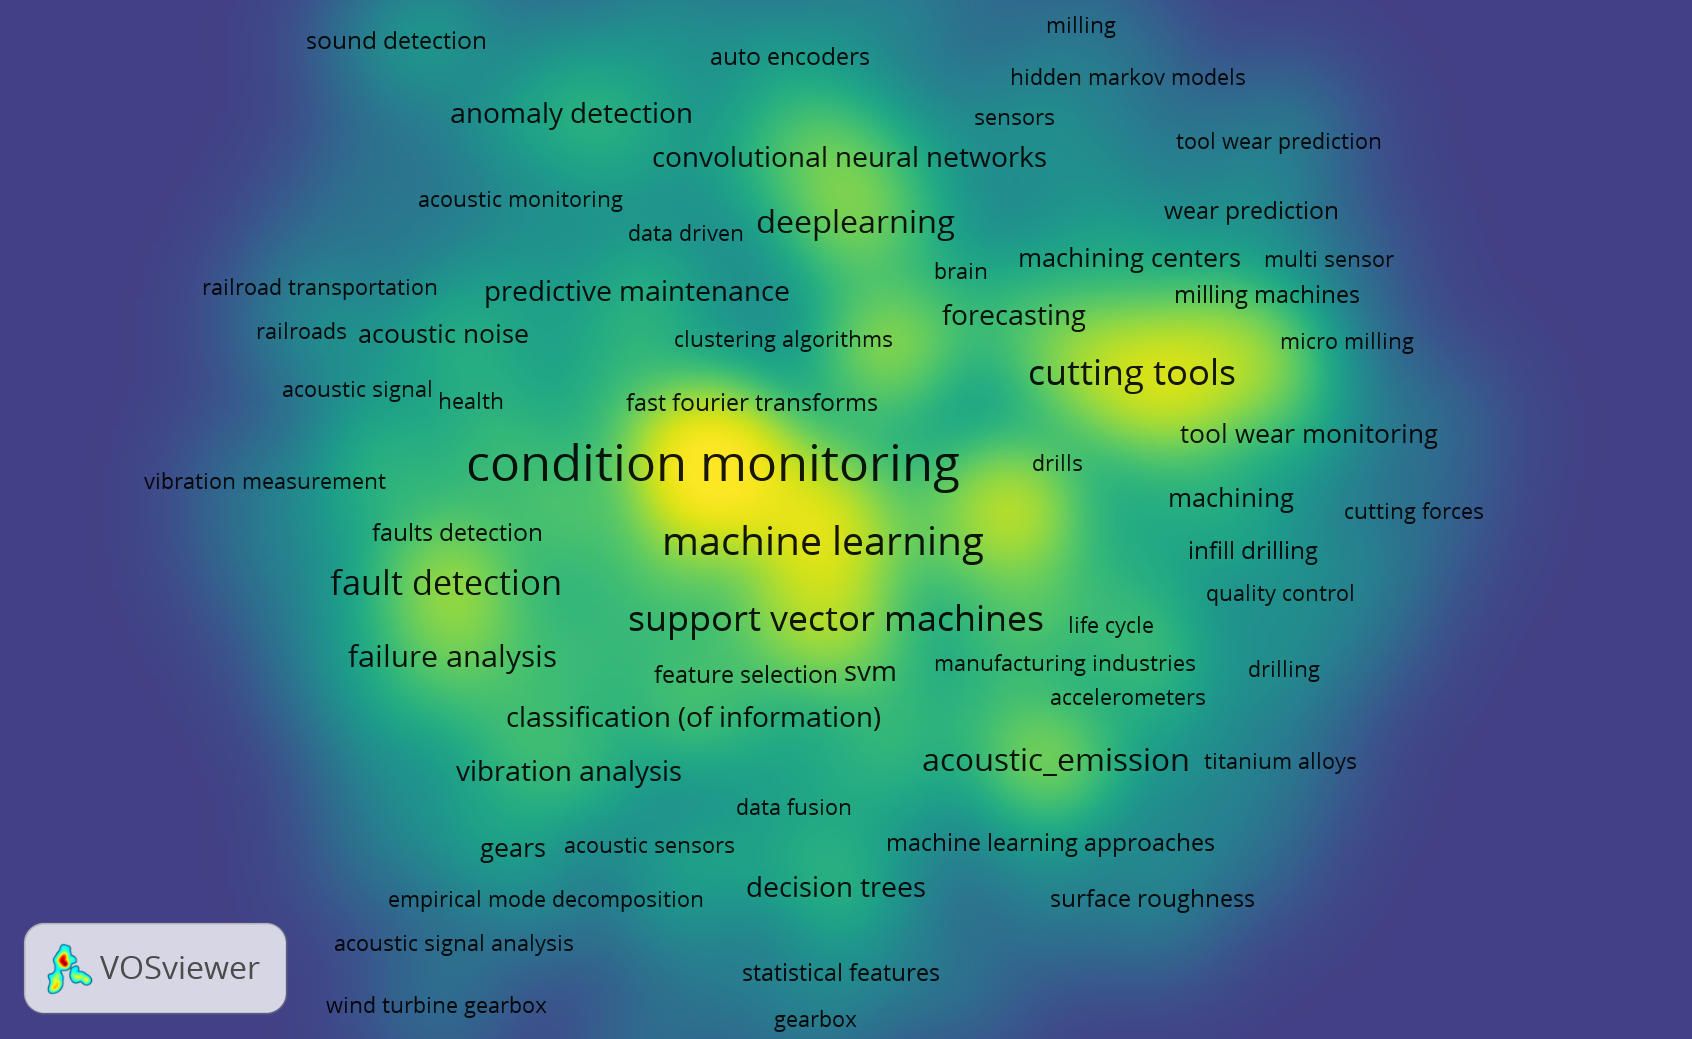
\includegraphics[width=0.85\textwidth]{figures/img_000.png}
\caption{Mapa de densidad en VOSviewer basado en palabras clave de t\'{i}tulo y resumen (corpus SCOPUS, 2010--2026). Los puntos calientes corresponden a: (i)~transformadas tiempo-frecuencia (CWT/FFT), (ii)~modelos de clasificaci\'{o}n (SVM, CNN) y (iii)~sensores y dominios industriales.}
\end{figure}

La Figura 2, complementa y matiza lo visto en la Figura 1 dado que al representar las palabras clave que los propios autores eligen declarar explícitamente, el mapa de red resalta la intención declarada de los estudios. En este mapa aparecen de forma prominente nodos centrales como monitorización de condición (\textit{condition monitoring}) y emisión acústica (\textit{acoustic emission}), así como agrupamientos dedicados a técnicas (por ejemplo: support vector machines y decision trees) y a objetivos prácticos (fault detection, predictive maintenance). La red revela que, aunque los artículos emplean a menudo transformadas y descriptores técnicos, los autores suelen marcar sus contribuciones con términos más generales (monitorización, detección, máquinas de corte, etc), por lo que el mapa de palabras clave de autor sirve mejor para mostrar la perspectiva aplicada y los problemas que la comunidad pretende resolver.

\begin{figure}[htbp]
\centering
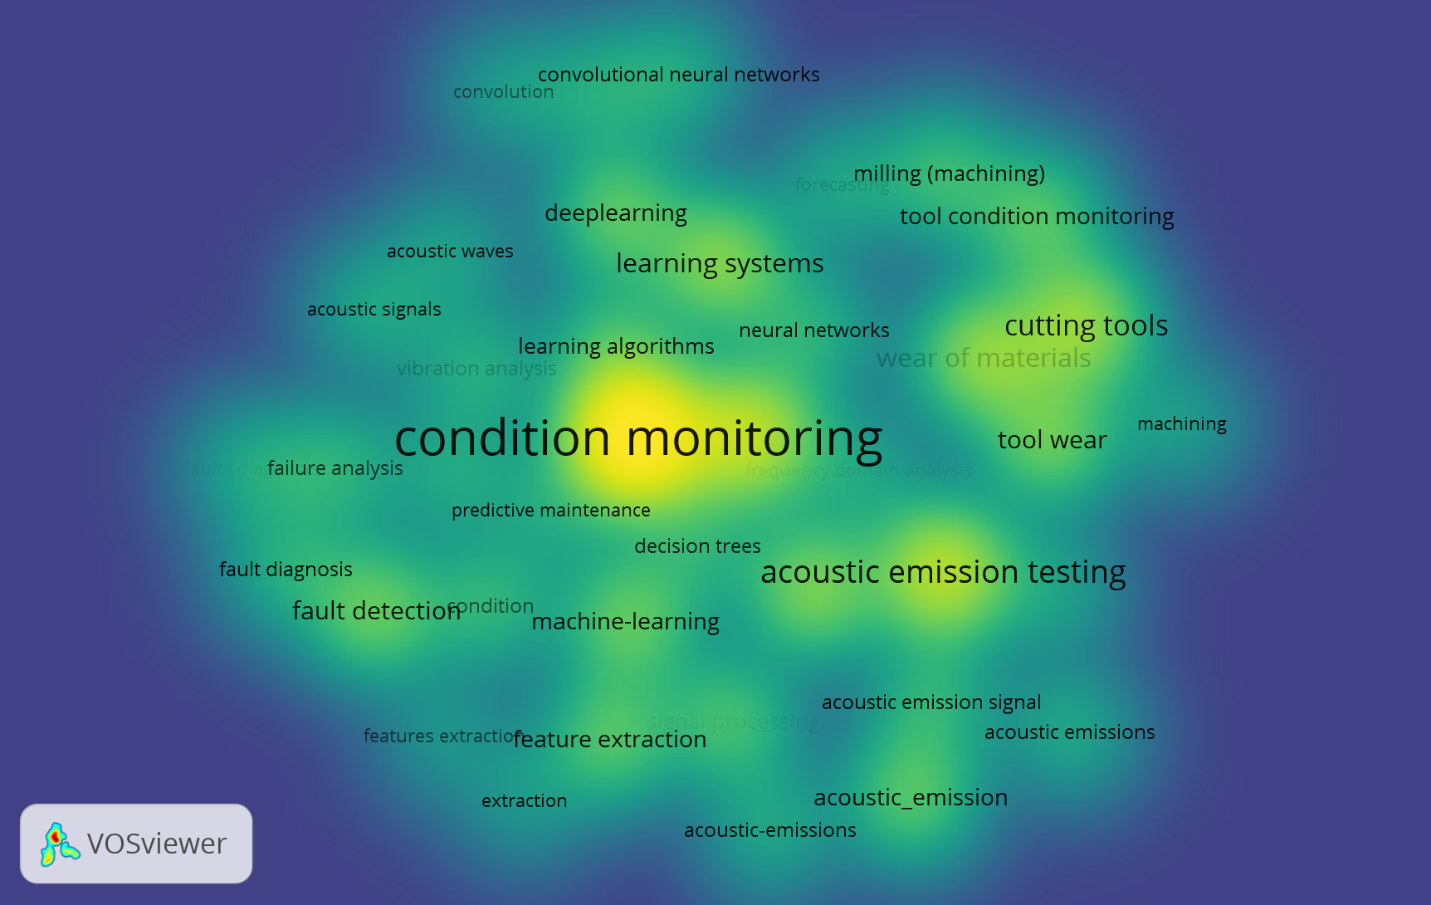
\includegraphics[width=0.85\textwidth]{figures/img_001.png}
\caption{Mapa de red en VOSviewer basado en palabras clave declaradas por los autores (n\'{u}cleos: \textit{condition monitoring}, \textit{acoustic emission}, SVM, CNN).}
\end{figure}

La comparación entre ambas figuras aporta varias conclusiones útiles para la tesis. En primera instancia, las transformadas tiempo-frecuencia (CWT/FFT) y las métricas de energía (RMS, energía wavelet, bandas mel) emergen como características recurrentes en los resúmenes, por lo que constituyen un punto de partida razonable y robusto para la extracción de variables. En segunda instancia, la presencia simultánea de SVM y Random Forest como nodos frecuentes indica que estos algoritmos funcionan como líneas base (\textit{baselines}) metodológicas en la literatura; su uso permite comparar resultados con estudios previos y facilita la interpretabilidad mediante importancias de variable (\textit{feature importances}) y pruebas de permutación (\textit{permutation importance}). En tercera instancia, la aparición de aprendizaje profundo (CNN) en Figura 1 sugiere una vía secundaria: cuando exista volumen suficiente de datos y recursos de cómputo , explorar modelos sobre espectrogramas (o imágenes CWT) puede mejorar captura de patrones locales y transitorios, aunque con menor interpretabilidad inmediata.

\clearpage
\chapter{Rediseño del ensayo}

El rediseño del ensayo busca establecer un protocolo reproducible que vincule cambios físicos en la interfaz herramienta--viruta con huellas detectables en la señal acústica y con medidas auxiliares (imágenes, caudal, vibración) que aumentan la fiabilidad del diagnóstico. Se parte de la hipótesis física de que los modos de desgaste (abrasión, adhesión, difusión, deformación plástica, etc.) modifican la energía, la distribución espectral y la estructura temporal de la señal acústica y que esas modificaciones son trazables y cuantificables

Metodológicamente, el capítulo se apoya en principios de diseño experimental: control y bloqueo de fuentes mayores de variación, tratamiento explícito de factores difíciles de cambiar (\textit{hard-to-change}), y registro sistemático de versiones y metadatos para facilitar comparaciones y adaptaciones futuras . Además, prioriza la representatividad de los datos mediante diversidad de sensores y conservación de formatos sin compresión para preservar transitorios relevantes a la detección.

A continuación, la sección 3.0.2 presenta el marco padre ---filosofía, criterios generales de diseño, y reglas de trazabilidad--- y la sección 3.0.3 documenta la adaptación concreta al lote experimental actual: montaje, sujeción, verificación, factores y plan de muestreo. El lector encontrará allí los procedimientos operativos, las comprobaciones de control y las reglas de versionado necesarias para mantener la coherencia entre lotes y facilitar la integración de nuevos ensayos en la base de datos.

La Figura~\ref{fig:estructura-estudio} sintetiza el flujo completo del trabajo: a la izquierda se ubican los componentes del rediseño del ensayo (taladrado, herramienta de corte, pieza de trabajo, máquina-herramienta, mecanismo de sujeción y parámetros de corte); en el centro, la cadena de adquisición y procesamiento de la señal acústica (sensor, módulo NI-9234 sobre cDAQ-9174, equipo de cómputo, conversión a forma de onda, eliminación de ruido y representación tiempo--frecuencia mediante espectrogramas); y a la derecha, las salidas del análisis ---valor eficaz, profundidad taladrada y vida útil de la herramienta--- que alimentan la etapa final de clasificación con TensorFlow para construir la base de conocimiento sobre el nivel de desgaste.

\begin{figure}[htbp]
\centering

\includegraphics[width=0.92\textwidth,keepaspectratio]{{figures/descripcion geenral de los pasos del ensayo}.png}
\caption[Estructura general del estudio]{Estructura general del estudio y descripción de los pasos del ensayo: rediseño (preparación del material y la herramienta, verificación del montaje y los parámetros de corte), adquisición y procesamiento (ejecución de la rutina de taladrado con registro multimodal ---audio NI, ESP32, microscopio---) y análisis y clasificación (volcado del manifiesto, etiquetado y despliegue de los modelos). El diagrama articula el orden lógico de los capítulos del informe y actúa como lista de verificación para el operario.}
\label{fig:estructura-estudio}
\end{figure}

\subsection{Definiciones operativas}

Unidad experimental primaria (entre-brocas): cada broca sometida a un conjunto de condiciones experimentales (factores y niveles) constituye la unidad experimental primaria. Las observaciones repetidas (agujeros sucesivos perforados con la misma broca) son mediciones anidadas dentro de la unidad experimental y deberán modelarse como series correlacionadas.

Esta jerarquía (broca $\rightarrow$ agujeros) obliga a emplear modelos mixtos con efectos aleatorios para la broca/sesión y efectos fijos para los factores controlados, tal como recomiendan textos de Diseño de Experimentos (DoE) para diseños anidados y medidas repetidas 

\subsection{Diseño experimental padre propuesto}

\subsubsection{Propósito y filosofía}

El protocolo padre define la columna vertebral del experimento: metadatos obligatorios, procedimientos de calibración y extracción de características “ancla”, reglas de bloqueo y estructuras de diseño para factores difíciles de cambiar (\textit{hard-to-change}). Este marco prioriza la reproducibilidad, la trazabilidad y la comparabilidad entre lotes experimentales. Se apoya en principios de diseño de experimentos y en la literatura sobre monitoreo acústico y aprendizaje automático (Montgomery, 2013; Groover, 2007; Géron, 2023).

\subsubsection{Elementos obligatorios del manifiesto (manifest)}

Cada registro de captura incluye un manifiesto mínimo que acompaña al archivo raw (WAV PCM): identificador único, fecha/hora UTC, frecuencia de muestreo (fs), ganancia y preamplificador, modelo de micrófono y número de serie, distancia micrófono--herramienta, versión del firmware/DAQ, versión del pipeline, checksum del archivo, condiciones de corte (RPM, avance, profundidad), lote de material y nota sobre alineación o incidencias. Estos campos permiten agrupar y filtrar datos para análisis comparables.

\subsubsection{Características anclas de calibración y control de calidad (QC).}

En cada sesión se graban señales de referencia para tono (\textit{chirp}) de banda ancha y toma de ruido de fondo, además de una toma con husillo sin carga. Estas grabaciones facilitan la evaluación de la Relación Señal Ruido (SNR), calibraciones de escala y la detección de cambios instrumentales entre sesiones. Se registra SNR por banda y se archiva un informe corto de QC.

\subsubsection{Lista de características “ancla”}

Se extraen siempre y de la misma forma un conjunto mínimo de características por archivo: RMS, RMS (dB), peak, centroid, rolloff, spectral\_bandwidth, zcr, mfcc\_0, mfcc\_1, mel\_total\_energy, wavelet\_total\_energy, spectral\_flatness, spectral\_contrast, chroma\_mean, chroma\_std, tonnetz\_0, harmonic\_percussive\_ratio, crest\_factor, onset\_rate, tempo, duration. Estas características ancla exploratorias garantizan comparabilidad aun cuando se añaden características experimentales.

\subsubsection{Estructura de diseño y tratamiento de factores hard-to-change.}

Cuando un factor resulta costoso de variar (tipo de bancada, sujeción, marca de micrófono), se lo trata como whole-plot en un diseño anidado (split-plot / nested). Los factores fácilmente manipulables (RPM, avance, caudal) se asignan como sub-plots dentro de cada whole-plot. El análisis emplea modelos de efectos mixtos para separar variación entre whole-plots y dentro de sub-plots \cite{montgomery2013}.

\subsubsection{Pilotos y etapa secuencial}

Antes de ampliar un lote, se ejecutan pruebas de adquisición de la señal acústica para estimar varianzas intra e inter-broca. Con esas estimaciones se realiza un cálculo de potencia (power analysis) para fijar número de brocas por celda y número de agujeros por broca. El enfoque secuencial permite optimizar recursos y evitar sobredimensionar diseños exploratorios, donde el objeto principal del mismo está en obtener un registro inicial base para la determinación del estado de la configuración del ensayo (mediante comparación de históricos).

\subsubsection{Registro de cambios (versionado)}

Toda modificación de hardware o cadena de elementos de procesamiento de datos conectados en serie (\textit{pipeline}) queda registrada en el manifiesto y en un registro de cambios (\textit{changelog}) con versión. Cambios instrumentales generan la obligación de realizar un experimento puente (\textit{bridge experiment}) para estimar desplazamientos instrumentales (\textit{batch effects}).

\subsubsection{Validación y métricas}

La validación de modelos respeta la independencia de grupos naturales (Group-aware CV, leave-one-broca-out). Las métricas principales son la puntuación Macro F1, la cual una métrica de múltiples etiquetas o clases para evaluaciones de calidad de inteligencia artificial y Área Bajo la Curva (AUC) para clasificación; tamaños de efecto ($\eta$$^2$, d de Cohen) y distribuciones robustas para decisiones de selección de características. La interpretabilidad incorpora importancia de permutación (\textit{permutation importance}) y el método de Explicaciones Aditivas de Shapley (SHAP) como complemento para priorizar características relevantes.

\subsection{Factores experimentales y niveles para diseño hijo}

Los factores incluidos se seleccionan por su vínculo directo con los mecanismos de desgaste en la interfaz herramienta-viruta y por su disponibilidad en el montaje actual. Se explica además como se medirá cada factor y qué papel físico juega en el proceso de desgaste.

\subsubsection{Máquina herramienta}

Se emplea el centro de mecanizado Leadwell V-20 (Figura 4), ubicado en el laboratorio de sistemas flexibles de la Escuela de Ingeniería Mecánica de la Universidad Industrial de Santander. Esta máquina, en buenas condiciones de funcionamiento, garantiza repetitividad en los ensayos y calidad en las señales capturadas. Además, al ser operada mediante comandos programados, permite realizar las pruebas de manera eficiente. Sus principales características se presentan en la Tabla 1.


\begin{figure}[htbp]
\centering
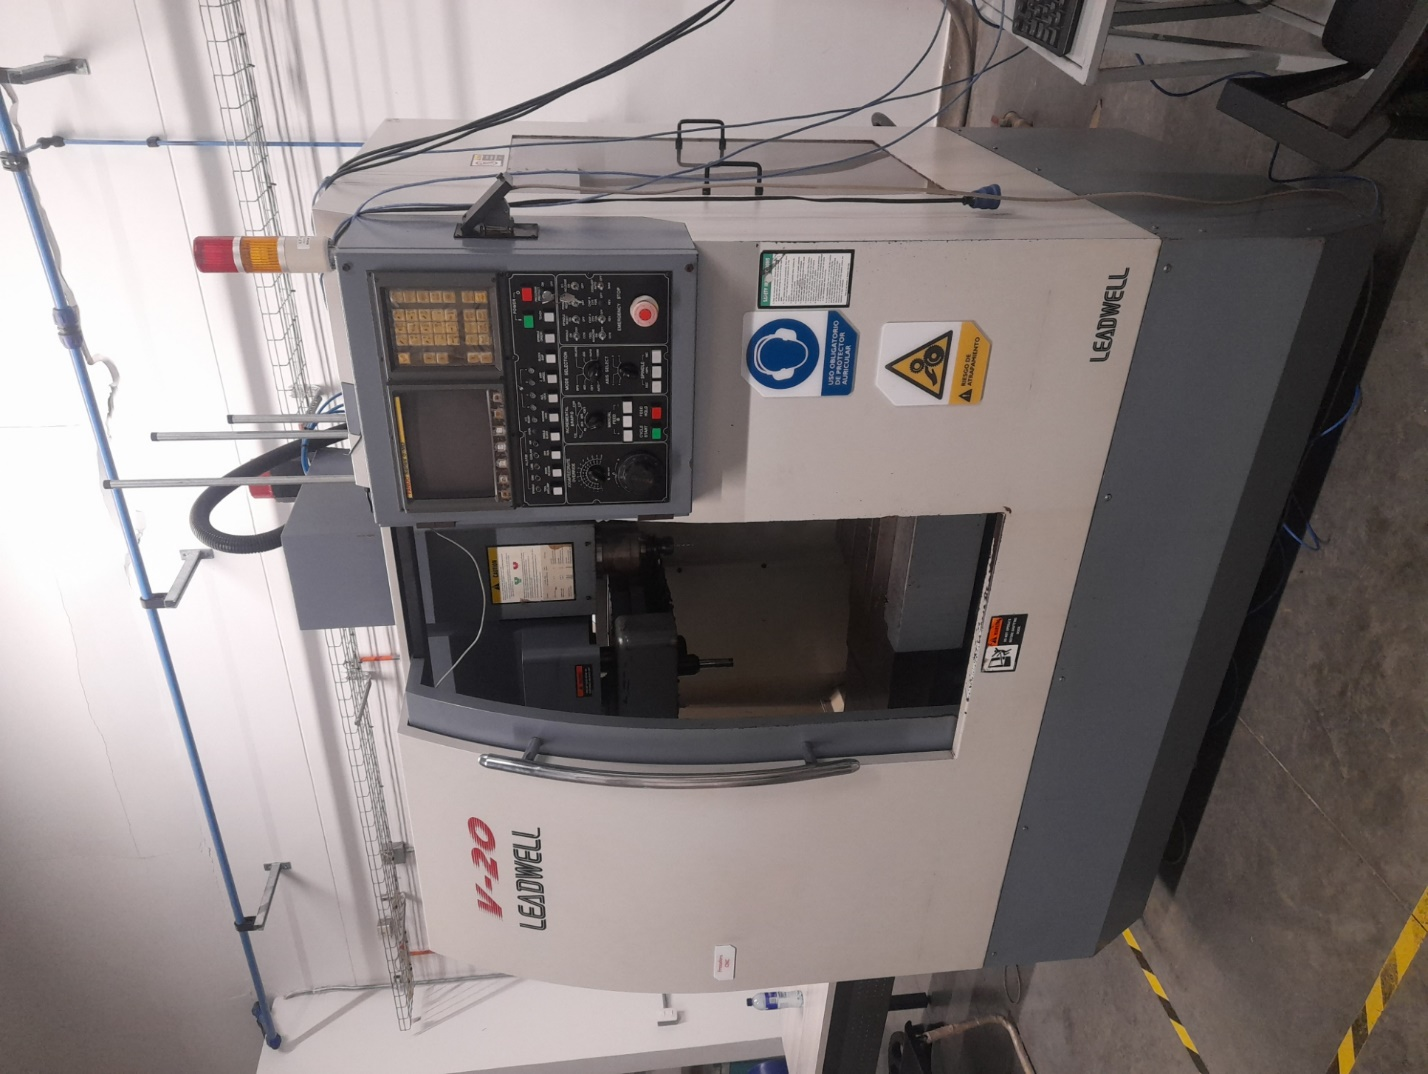
\includegraphics[width=0.6\textwidth,keepaspectratio]{figures/img_008.jpg}
\caption{Centro de mecanizado Leadwell V-20 del Laboratorio de Sistemas Flexibles, Escuela de Ingeniería Mecánica, Universidad Industrial de Santander (Cap~4).}
\end{figure}

\begin{table}[htbp]
\centering
\small
\caption{Caracter\'{i}sticas t\'{e}cnicas del centro de mecanizado Leadwell V-20.}
\label{tab:leadwell-v20}
\begin{tabularx}{\textwidth}{X X X}
\toprule
Caracter\'{i}stica & Medida & Unidad \\
\midrule
Recorrido eje X & 510 & Mil\'{i}metros \\
Recorrido de eje Y & 350 & Mil\'{i}metros \\
Recorrido de eje Z & 400 & Mil\'{i}metros \\
Mesa &  &  \\
Medida & 600$\times$350 & mm$^2$ \\
M\'{a}ximo peso de carga & 200 & Kilogramos \\
\bottomrule
\end{tabularx}
\end{table}

\subsubsection{Pieza de trabajo}


\begin{table}[htbp]
\centering
\small
\caption{Composici\'{o}n qu\'{i}mica del acero AISI-SAE~4140 seleccionado para el Cap.~4 (fracciones en masa, \,\%).}
\label{tab:comp-4140-cap4}
\begin{tabularx}{\textwidth}{X X X X X X X}
\toprule
C & Mn & Si & Cr & Mo & S & P \\
\midrule
0{,}38--0{,}43 & 0{,}75--1{,}0 & 0{,}15--0{,}35 & 0{,}80--1{,}10 & 0{,}15--0{,}25 & M\'{a}x. 0{,}040 & M\'{a}x. 0{,}035 \\
\bottomrule
\end{tabularx}
\end{table}

Desde la perspectiva de desgaste y su detección acústica, las propiedades mencionadas ---composición, dureza y tratamiento de suministro--- condicionan los mecanismos físico-químicos que rigen la generación de ruido en la interfaz herramienta--viruta (abrasión, adhesión, difusión y deformación plástica). Por ejemplo, una mayor dureza relativa entre pieza y herramienta tiende a favorecer modos de abrasión, que se reflejan en variaciones continuas de energía y contenido espectral ; cambios en temperatura y lubricación (influenciados por el refrigerante) facilitan procesos de adhesión o difusión local que también alteran la estructura temporal del audio. Por ello, la conservación de la misma especificación de material y proveedor que en el estudio histórico es un requisito para poder atribuir cambios en las señales a variaciones experimentales controladas y no a diferencias de materia prima.

\begin{table}[htbp]
\centering
\caption{Geometr\'{i}a de la pieza de trabajo: disco de acero SAE~4140 para el Lote~II.}
\label{tab:pieza-trabajo}
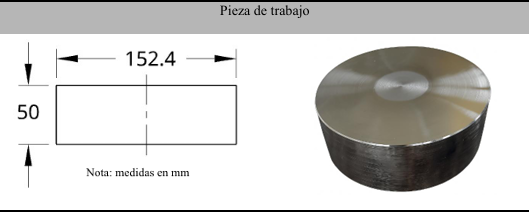
\includegraphics[width=0.85\textwidth]{figures/tabla_03.png}
\end{table}

Posteriormente, se efectuó una inspección superficial mediante micrografía sencilla, identificando dos zonas diferenciales a simple vista en las caras de los discos que sirvieron como referencia para la selección de la sujeción. En la Figura 5 se observa el proceso de refrentado además de que se presentan los resultados superficiales obtenidos tras la operación.


\subsubsection{Herramienta de corte}

Con el fin de garantizar la coherencia entre la dureza del material de trabajo y la resistencia de la herramienta de corte, se tomaron precauciones iniciales orientadas a preservar la relación de especímenes establecida en el trabajo previo. En este contexto, se seleccionaron brocas Dormer A100\textbf{ }de 6 mm y 8 mm Figura 8. A pesar de que este modelo había dejado de estar disponible en el área metropolitana de Bucaramanga, se realizaron gestiones adicionales para adquirir las mismas referencias, contactando proveedores en otros departamentos del país que podían suministrarlas bajo pedido.


\begin{figure}[htbp]
\centering
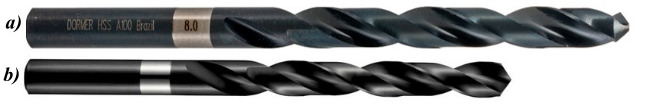
\includegraphics[width=0.55\textwidth,keepaspectratio]{figures/img_016.png}
\caption{Brocas helicoidales Dormer A100 HSS de 6\,mm y 8\,mm seleccionadas para los ensayos del Lote~II por compatibilidad con el material previo \protect\citeA{orejarena2014}.}
\end{figure}

Tras su implementación en los primeros ensayos, se identificó la necesidad de ampliar el número (cantidad) de brocas empleadas, ya que los cambios representativos en la configuración experimental ---particularmente en el sistema de sujeción y en la búsqueda de introducir variaciones controladas--- podían comprometer la construcción de una base de conocimiento robusta, evitando que los modelos de aprendizaje automático se entrenaran de manera sesgada hacia una única configuración de pruebas.

Con este propósito, se autorizó la inclusión de un segundo tipo de broca de la misma marca, pero de mayor disponibilidad en el mercado local. Así, se incorporaron brocas Dormer A114 Figura 9, que complementaron la estrategia experimental y se aseguró la continuidad del proyecto sin afectar la comparabilidad de los resultados.

\begin{figure}[htbp]
\centering
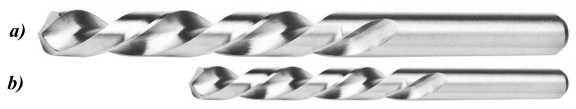
\includegraphics[width=0.55\textwidth,keepaspectratio]{figures/img_017.png}
\caption{Brocas helicoidales Dormer A114 en di\'{a}metros 6\,mm y 8\,mm, incorporadas como complemento al modelo A100 ante limitaciones de disponibilidad local.}
\end{figure}

\paragraph{Geometría de las brocas}

La Tabla 4 establece las dimensiones y característica entre ambas referencias de brocas y permite notar diferencias notables de entrada como el recubrimiento que no trae la referencia A114 comparación a la A100. 


\begin{table}[htbp]
\centering
\caption{Dimensiones y caracter\'{i}sticas comparativas de las brocas Dormer A100 y A114 en di\'{a}metros 6\,mm y 8\,mm.}
\label{tab:brocas-dim}
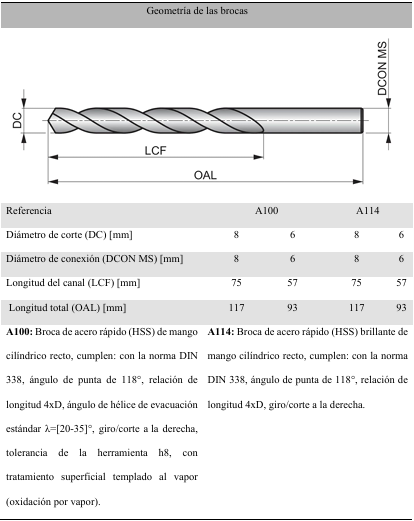
\includegraphics[width=0.85\textwidth]{figures/tabla_04.png}
\end{table}

\paragraph{Montaje de la herramienta}

El montaje seleccionado utiliza un cono BT40 alojado en el husillo del centro de mecanizado y un porta-pinza tipo ER (Figura 10). La pinza ER, también llamada collet (pinza elástica), se introduce en el porta-pinza; al apretar la tuerca, la pinza se comprime y sujeta axial y radialmente el vástago cilíndrico de la broca. Para las brocas de 6 y 8 mm se emplean pinzas del rango correspondiente que garantizan contacto total sobre el vástago, evitando el uso de tornillos de fijación tipo tornillo de tope (\textit{set-screw}) que generan excentricidad y daños en el vástago.


\begin{figure}[htbp]
\centering
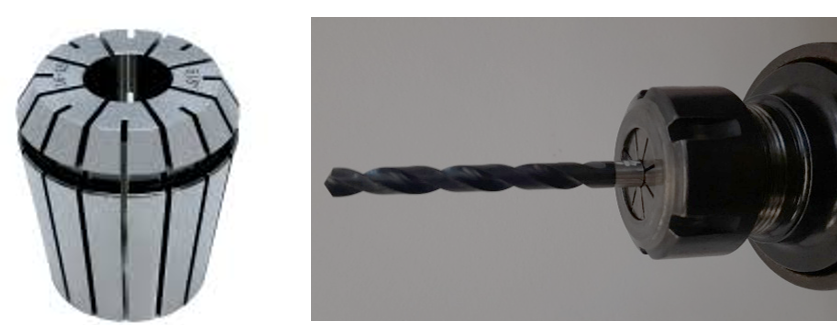
\includegraphics[width=0.65\textwidth,keepaspectratio]{figures/img_019.png}
\caption{Montaje de la herramienta con (a) pinza ER y (b) porta-pinza ER instalados en el husillo del centro de mecanizado Leadwell V-20.}
\end{figure}

Desde la perspectiva mecánica y experimental, la elección de pinzas ER responde a criterios prácticos y de señal que mejoran la concentricidad y reducen el descentrado radial (\textit{run-out}), lo que disminuye fuentes periódicas de vibración que contaminan la señal acústica; ofrecen mayor rigidez y fuerza de sujeción, reduciendo micro-movimientos y el riesgo de deslizamiento, y facilitan la repetibilidad entre montajes (misma profundidad de asiento y torque de apriete). Además, comparadas con un mandril tipo Jacobs (mandril con mordazas), las pinzas ER tienden a introducir menor masa desequilibrada en la periferia del porta-herramientas y permiten cambios rápidos de herramienta sin perder concentricidad.

No obstante, el sistema collet de porta-pinza también exige controles rutinarios porque cualquier variación en rigidez, desgaste o balance afecta la firma acústica. Para mitigar riesgos y preservar la comparabilidad entre lotes de ensayo se implementan medidas operativas y de registro: antes de iniciar cada sesión se verifica el asiento de la pinza y la ausencia de virutas o suciedad en la zona de contacto; se controla el par de apriete con llave de torque calibrada (anotar valor y operador en el manifiesto). se puede medir el descentrado radial con comparador de carátula (DTI) y se registra; y se mantiene un registro de uso/vida útil de cada collet para reemplazar piezas que muestren desgaste. Asimismo, se realizan ensayos piloto de referencia acústica que incluyen, al menos, (a) grabación del husillo sin porta-herramientas, (b) grabación con porta-herramientas y collet montados sin broca y sin carga, y (c) grabación con broca nueva montada y sin corte ---estas señales de referencia permiten diagnosticar cambios instrumentales posteriores y facilitar la normalización o recalibración de las series.

\subsubsection{Parámetros de corte}
\label{subsec:params-corte}

Los parámetros de corte se determinaron a partir del selector de herramientas Dormer y se contrastaron con el cálculo teórico para verificar la coherencia con los principios de remoción de material \cite{groover2007}. La Figura~\ref{fig:dormer-selector} reproduce la página del catálogo Dormer A100 (serie corta) con los valores recomendados para los diámetros 6\,mm y 8\,mm en acero SAE~4140, fuente original adoptada por \citeA{orejarena2014} para fijar los parámetros del ensayo histórico. Para garantizar la comparabilidad entre lotes, este trabajo conserva la misma referencia comercial y reproduce los cálculos en condiciones equivalentes.

\begin{figure}[htbp]
\centering
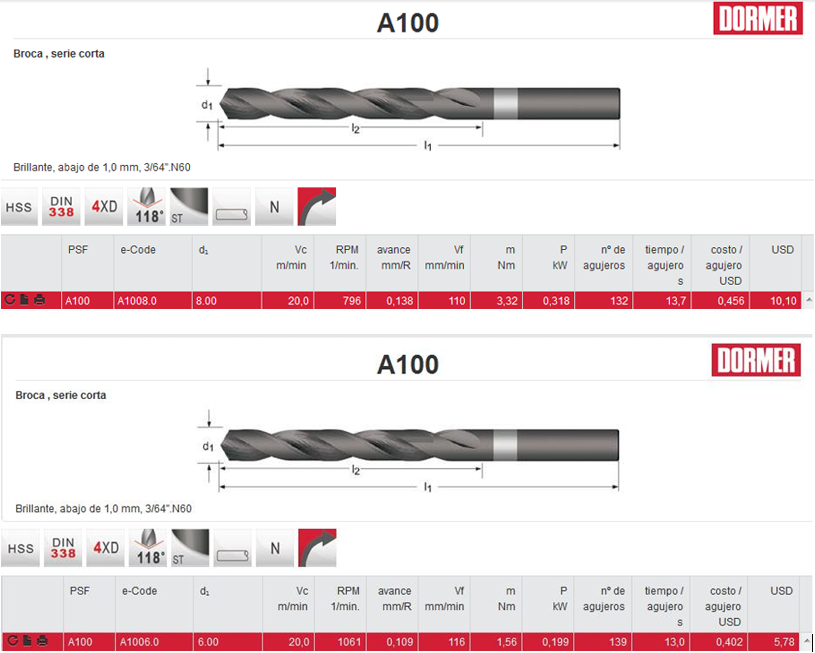
\includegraphics[width=0.85\textwidth,keepaspectratio]{figures/img_020.png}
\caption[Selector de herramienta Dormer A100]{Selector de herramienta Dormer A100 (serie corta, HSS, recubrimiento brillante) para acero SAE~4140 en di\'{a}metros 6\,mm (inferior) y 8\,mm (superior). Se observan los valores recomendados de velocidad de corte ($v_c$), revoluciones por minuto, avance por revolución, avance lineal, par, potencia y vida nominal de la herramienta.}
\label{fig:dormer-selector}
\end{figure}

\paragraph{Datos de partida (broca A100, 8\,mm).}
A partir del selector y de la convención adoptada en el estudio de \citeA{orejarena2014} se fijan: diámetro $d = 8$\,mm, velocidad de corte $v_c = 20$\,m/min, avance por revolución $f_r = 0{,}138$\,mm/rev, profundidad de taladrado $L = 25$\,mm (agujero ciego) y potencia de referencia $P = 0{,}318$\,kW. Con estos datos se calculan los cuatro parámetros operativos siguientes.

\paragraph{Revoluciones por minuto.}
La velocidad de rotación del husillo se obtiene a partir de la velocidad de corte y el diámetro de la broca:
\begin{equation}
\label{eq:rpm}
N = \frac{1000\, v_c}{\pi\, d}
\end{equation}
Sustituyendo, $N = \dfrac{1000 \cdot 20}{\pi \cdot 8} = 795{,}77 \approx 796$\,rpm, valor coincidente con el del selector Dormer.

\paragraph{Velocidad lineal de avance.}
A partir del avance por revolución y la velocidad de giro:
\begin{equation}
\label{eq:avance-lineal}
v_f = f_r \cdot N
\end{equation}
$v_f = 0{,}138 \cdot 796 = 109{,}8 \approx 110$\,mm/min.

\paragraph{Tiempo por agujero ciego.}
Para una profundidad $L = 25$\,mm:
\begin{equation}
\label{eq:tiempo-agujero}
t_h = \frac{L}{v_f}
\end{equation}
$t_h = \dfrac{25}{110} = 0{,}227$\,min $\approx 13{,}7$\,s por agujero, valor consistente con la columna ``tiempo por agujero'' del catálogo Dormer.

\paragraph{Par (torque) en el husillo.}
A partir de la potencia mecánica disponible y la velocidad de rotación:
\begin{equation}
\label{eq:torque}
T = \frac{60\,000\, P}{2 \pi N}
\end{equation}
$T = \dfrac{60\,000 \cdot 0{,}318}{2\pi \cdot 796} = 3{,}82$\,N$\cdot$m $\approx 3{,}32$\,N$\cdot$m según los redondeos del catálogo, valor consistente con la práctica de taller para acero al carbono medio.

De forma análoga se aplicaron las Ecuaciones~\eqref{eq:rpm}--\eqref{eq:torque} a la broca de 6\,mm y a la referencia complementaria Dormer A114 incorporada al Lote~II (manteniendo $v_c = 20$\,m/min y $f_r$ ajustado al diámetro según el selector y los manifiestos del ensayo). Los resultados se resumen en la Tabla~\ref{tab:params-corte-cap4}.

\begin{table}[htbp]
\centering
\small
\caption{Par\'{a}metros de corte calculados para brocas Dormer A100 y A114 de 6\,mm y 8\,mm en acero SAE~4140 (velocidad de corte constante $v_c = 20$\,m/min, profundidad $L = 25$\,mm).}
\label{tab:params-corte-cap4}
\begin{tabularx}{\textwidth}{l c c c c c c}
\toprule
Referencia & $d$ (mm) & $N$ (rpm) & $f_r$ (mm/rev) & $v_f$ (mm/min) & $t_h$ (s) & $T$ (N$\cdot$m) \\
\midrule
Dormer A100 & 6 & 1061 & 0{,}109 & 116 & 12{,}9 & 1{,}35 \\
Dormer A100 & 8 & 796  & 0{,}138 & 110 & 13{,}7 & 3{,}82 \\
Dormer A114 & 6 & 1061 & 0{,}109 & 116 & 12{,}9 & 1{,}35 \\
Dormer A114 & 8 & 796  & 0{,}138 & 110 & 13{,}7 & 3{,}82 \\
\bottomrule
\end{tabularx}
\end{table}

Los valores de la Tabla~\ref{tab:params-corte-cap4} se validaron contra los manifiestos de los ensayos E8--E14 (por ejemplo, 1\,061\,rpm y 116\,mm/min en las brocas de 6\,mm, coincidentes con los del selector Dormer para $v_c = 20$\,m/min). Al comparar los valores calculados con las recomendaciones del selector Dormer-Pramet se observa que, tras el redondeo práctico utilizado en taller, ambos coinciden. Esta concordancia valida los ajustes experimentales propuestos tanto frente a la referencia comercial como desde el punto de vista teórico \cite{groover2007}, y respalda la decisión de conservar los mismos parámetros de corte que el experimento histórico para preservar la comparabilidad de las firmas acústicas.

\subsubsection{Distribución y secuencia de taladrado}

Para maximizar la potencia estadística del experimento y favorecer la detección de los efectos físicos relevantes sobre el desgaste de la broca (abrasión, adhesión, difusión y deformación plástica), se decidió limitar la variación en la trayectoria de taladrado manteniendo una única secuencia: espiral. Esta decisión se fundamenta en razones experimentales, prácticas y estadísticas:

\paragraph{Evidencia previa: baja influencia de la trayectoria en la señal acústica}

 Estudios previos en la línea de trabajo \cite{orejarena2014} mostraron que los cambios de trayectorias diseñadas ---espiral, lineal o mixta--- no produjeron diferencias directas y consistentes en las firmas acústicas que fueran comparables en magnitud con otras fuentes de variación (por ejemplo, dureza del material, condiciones de sujeción o ruido estructural). Dado que la trayectoria no se mostró como una fuente dominante de variación acústica, su inclusión como factor experimental primario aportaría poco a la potencia para detectar efectos reales de desgaste y, al contrario, introduciría complejidad innecesaria.

\paragraph{Variabilidad de dureza del material: factor mayor y difícil de controlar}

Ensayos y mediciones (durómetro) indican que la dureza del lote de SAE/AISI 4140 presenta variaciones entre piezas y lotes del proveedor ; dichas variaciones responden a procesos de fabricación (fundición, bonificado, etc.) que no se pueden homogeneizar fácilmente en laboratorio. Cuando una fuente de variación (dureza) es grande y difícil de controlar, introducir otras fuentes menores (trayectorias múltiples) reduce la capacidad de detectar el efecto real de los factores de interés. Priorizar la reducción de factores experimentales controlables mejora la detectabilidad de efectos físicos verdaderos.

\paragraph{Principio de parsimonia en diseño experimental}

Para estimar efectos principales e interacciones con eficiencia estadística conviene mantener bajo número de factores irrelevantes o de bajo efecto. Reducir las fuentes de variación no informativas disminuye la varianza residual y aumenta la potencia para detectar diferencias asociadas a factores físicamente relevantes (rpm, avance, refrigeración, sujeción, sensor). Esta estrategia es coherente con los principios de planificación de experimentos , que promueven diseños parcimoniosos y el bloqueo/control de fuentes mayores de variación.

\paragraph{Beneficio estadístico: aumentar N efectivo y reducir varianza residual}

Al usar una sola secuencia se puede aumentar el número de agujeros por broca (más observaciones repetidas dentro de cada unidad experimental), lo que mejora la estimación de la curva de vida útil y reduce la varianza dentro-broca. Esto facilita emplear modelos jerárquicos (mixed-effects) donde la variación entre brocas se modela como efecto aleatorio y la evolución por agujero como observaciones anidadas.

\paragraph{Compromiso metodológico: mantener comparabilidad con histórico}

Mantener una única secuencia facilita la comparación con el dataset histórico , que ya tiene protocolos y patrones de sujeción distintos. La consistencia en la secuencia ayuda a minimizar diferencias metodológicas que dificulten la validación cruzada entre datasets.

\paragraph{Registro y control para futuras extensiones}

Aunque la trayectoria no se manipule como factor principal, se registrará la trayectoria (metadato en el manifiesto) y se conservarán copias crudas de audio y video. Así, si en el futuro se decide estudiar la trayectoria como factor, los datos permitirán análisis exploratorios o estudios adicionales sin comprometer los resultados primarios.

Con base en lo anterior, se define una nueva distribución de perforado que optimiza el aprovechamiento del material: 178 agujeros para la broca de 8 mm (frente a 117 en el experimento original) y 292 agujeros para la broca de 6 mm (frente a 220). Las trayectorias y la secuencia de taladrado se diseña en Fusion 360 (CAD/CAM),\textbf{ }de Autodesk, que permite generar y verificar geométricamente las rutas y simular la mecanización tal y como se diseña en Fusion 360. Dado que Fusion no soporta la simulación directa a partir de G-code personalizado y presenta limitaciones para modificar y simular código propio, y además por la restricción de memoria de la Leadwell V-20 (problemas al ejecutar programas con más de $\approx$ 300 líneas), fue necesario introducir un paso intermedio de posprocesado del G-code. Para ello se empleó CIMCO Edit 8, que facilitó la modularización del programa mediante subprogramas: se creó un programa maestro que invoca fragmentos más pequeños, reduciendo la longitud de cada archivo enviado a la máquina y evitando envíos incompletos por la limitación de memoria.


Adicionalmente, el G-code final incorpora paradas programadas y cambios de referencia que posicionan la herramienta para la captura visual del filo (inspecciones por video/micrografía) en puntos predefinidos del ensayo. Esta estrategia permite construir de forma sistemática la serie temporal visual del desgaste sin interrumpir la automatización del ciclo de taladrado. Los detalles operativos y de integración (estructura de subprogramas, ejemplos de fragmentos de G-code, sincronización con la captura de video y el pipeline de procesamiento posterior) se describen con mayor profundidad en el capítulo siguiente. En conjunto, la nueva distribución y el flujo de posprocesado garantizan reproducibilidad, aprovechamiento del material y la capacidad de capturar evidencia visual periódica para el etiquetado y la correlación multimodal.

\subsubsection{Sujeción de la pieza de trabajo}

En el montaje del juego de experimentos previos  se detecta un problema con las bridas de dos tornillos: al sujetar la pieza por la cara superior reducen la superficie útil para taladrar y obligan a manipulaciones frecuentes que alargan los tiempos de preparación. Además, esas bridas se han obtenido mediante alquiler, lo que genera dependencia logística. El contacto localizado de este sistema tiende a crear puntos de apoyo que deforman la pieza o alteran la transmisión vibratoria, afectando las señales acústicas.


Como alternativa se adopta una copa de sujeción que apoya la pieza por la periferia, mostrada en la Figura~\ref{fig:copa-sujecion}, liberando la cara superior y permitiendo un mayor número de agujeros por disco. La copa aporta mayor rigidez y repetibilidad posicional, reduce holguras y facilita la incorporación de accesorios (casquetes, anillos, topes) sin invadir la zona de taladrado. Al ser un elemento propio del taller mejora la logística y la trazabilidad (es más sencillo documentar lotes y medir desviación de pieza (\textit{runou}t), desviación radial/axial y balance) antes del ensayo. Además, la sujeción periférica distribuye la transmisión vibratoria de modo más uniforme, lo que beneficia la comparabilidad de las firmas acústicas entre sesiones.

\begin{figure}[htbp]
\centering
\begin{minipage}{0.48\textwidth}\centering
\includegraphics[width=\textwidth,keepaspectratio]{figures/copa_sujecion_cad_real.png}\\
\small (a) Modelo CAD del conjunto copa--disco.
\end{minipage}\hfill
\begin{minipage}{0.48\textwidth}\centering
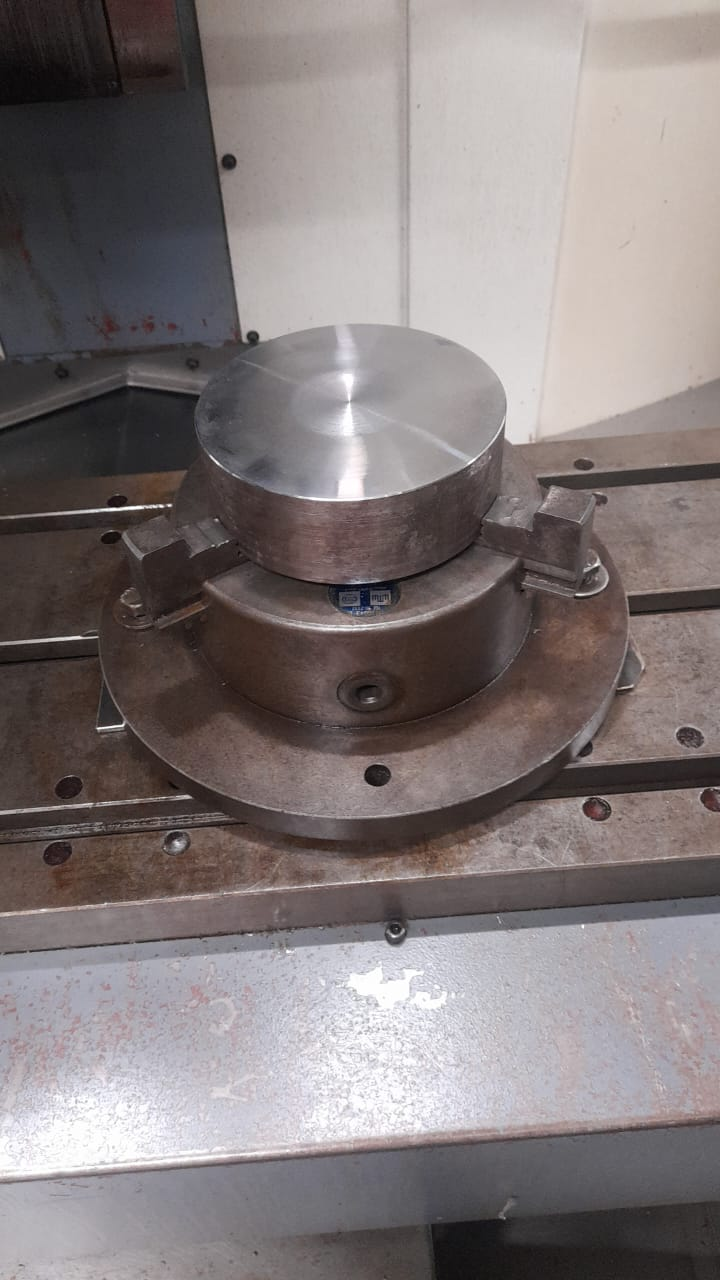
\includegraphics[width=\textwidth,keepaspectratio]{figures/copa_sujecion_foto.jpg}\\
\small (b) Copa instalada en la mesa del Leadwell V-20.
\end{minipage}
\caption[Copa de sujeci\'{o}n perif\'{e}rica propuesta]{Sistema de sujeci\'{o}n por copa perif\'{e}rica: (a)~modelo CAD con el disco encastrado y los puntos de apriete laterales y (b)~implementaci\'{o}n f\'{i}sica en la mesa del centro de mecanizado. La copa libera la cara superior del disco, ampl\'{i}a el n\'{u}mero de agujeros \'{u}tiles por pieza y homogeneiza la transmisi\'{o}n vibratoria respecto a la sujeci\'{o}n por bridas empleada en el Lote~I.}
\label{fig:copa-sujecion}
\end{figure}

Para contrastar con el esquema de bridas utilizado originalmente se documenta tambi\'{e}n el montaje alternativo por bridas escalonadas (Figura~\ref{fig:sujecion-bridas}), que sirvi\'{o} como configuraci\'{o}n de respaldo durante los primeros ensayos y permiti\'{o} descartar la hip\'{o}tesis de que la baja vida \'{u}til de las brocas respecto a \citeA{orejarena2014} se debiera a vibraciones introducidas por el soporte.

\begin{figure}[htbp]
\centering
\begin{minipage}{0.48\textwidth}\centering
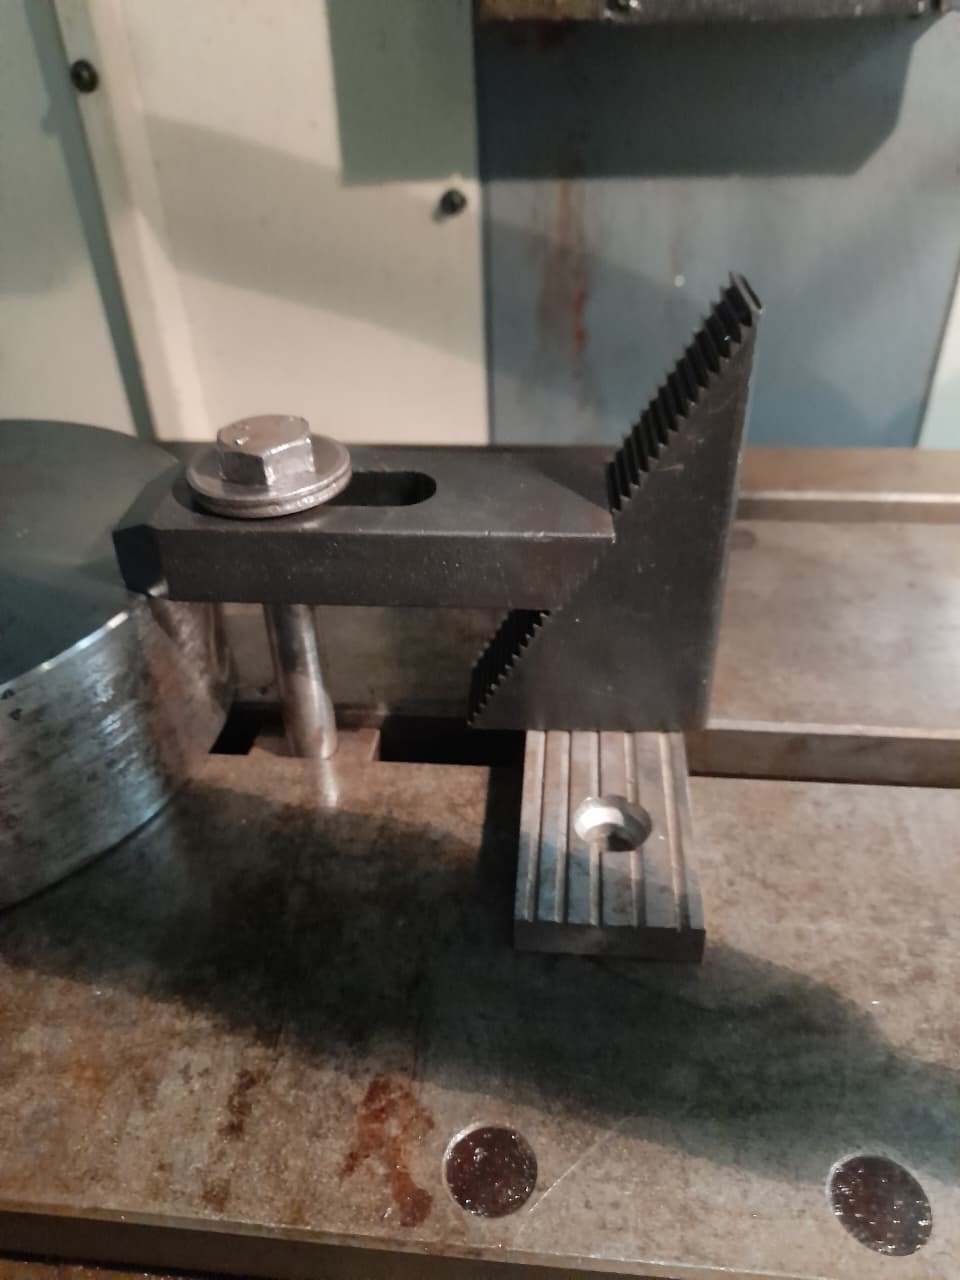
\includegraphics[width=\textwidth,keepaspectratio]{figures/sujecion_bridas_escalonadas.jpeg}\\
\small (a) Sujeci\'{o}n por bridas escalonadas.
\end{minipage}\hfill
\begin{minipage}{0.48\textwidth}\centering

\includegraphics[width=\textwidth,keepaspectratio]{{figures/material taladrado en sujecion de copa}.jpeg}\\
\small (b) Disco taladrado y retenido por la copa.
\end{minipage}
\caption[Sujeci\'{o}n alternativa por bridas vs.\ copa perif\'{e}rica]{Comparaci\'{o}n entre las dos estrategias de sujeci\'{o}n evaluadas: (a)~bridas escalonadas con par de tuercas en T y soportes dentados que aplican fuerza sobre dos superficies del material --- configuraci\'{o}n heredada del Lote~I---; y (b)~disco ya taladrado dentro de la copa perif\'{e}rica, donde se aprecia la cara superior libre de obst\'{a}culos y el patr\'{o}n espiral de agujeros ejecutado.}
\label{fig:sujecion-bridas}
\end{figure}

No obstante, su uso requiere de controles: si la copa no asegura paralelismo ni presión homogénea puede generar vibraciones y resonancias que degradan la relación señal/ruido. La desviación de una pieza y una sujeción insuficiente pueden provocar errores posicionales y deslizamientos. 

Para minimizar riesgos se exige una verificación previa y rutinaria: i) comprobar planitud y concentricidad con comparador de carátula (DTI) tras montar la copa, ii) ejecutar pruebas de balance y registro de vibraciones a baja velocidad para identificar resonancias iii) realizar ensayos de torque/forzado que aseguren ausencia de deslizamiento bajo condiciones de corte y iv) instalar juntas o escudos que desvíen refrigerante y protejan cableado y acoplamientos. Cada montaje queda fotografiado y documentado.

Desde la óptica del diseño experimental, la copa mejora la potencia estadística: al reducir la variación introducida por la sujeción se disminuye la varianza residual y se eleva la capacidad de detectar efectos reales del desgaste en las señales acústicas. El aumento del número de agujeros útiles por disco incrementa las observaciones anidadas dentro de cada broca, favoreciendo estimaciones robustas de la curva de vida útil y el empleo de modelos jerárquicos (efectos mixtos) que separan variación entre brocas y evolución dentro de la broca. Asimismo, la reproducibilidad posicional facilita la comparación con el dataset histórico y la ampliación consistente de la base de datos.

\subsection{Diseño experimental hijo}

\subsubsection{Contexto del lote}

El lote hijo toma como plataforma la configuración concreta: centro de mecanizado Leadwell V-20, piezas en AISI 4140 (dureza 28--32 HRC, ficha técnica en Apéndice~\ref{ap:ficha-aisi4140}), brocas Dormer A100 y A114 en diámetros 6 mm y 8 mm, sujeción mediante copa periférica y portaherramientas pinzas (\textit{collets})ER. La trayectoria de taladrado es espiral; profundidad por agujero 25 mm (agujero ciego). Los parámetros de corte se fijan con base en recomendaciones Dormer y cálculo teórico (ej.: Vc = 20 m/min, avance por rev según diámetro).

\subsubsection{Jerarquía experimental}

Unidad primaria: broca (entre-brocas). Observaciones anidadas: agujeros secuenciales perforados por la misma broca (dentro-broca). Se modela la jerarquía con efectos aleatorios para broca/sesión y efectos fijos para tratamiento (refrigeración, avance, RPM, tipo de broca).

\subsubsection{Bloqueo y aleatorización}

Se bloquea por lote de material y por sesión de laboratorio. Dentro de cada bloque, se asignan aleatoriamente las brocas a las celdas de tratamiento y se aleatoriza el orden de ejecución de brocas para mitigar efectos temporales (drift). Cuando la sujeción o portabrocas actúan como whole-plot, se asignan sub-ploteos para variaciones de RPM y avance.

\subsubsection{Replicación y plan de muestreo}

Se mantiene, como mínimo, 4 brocas por celda de tratamiento para estimar varianza entre-broca con suficiente robustez. Para la broca de 8 mm se registran 178 agujeros por broca y para la de 6 mm 292 agujeros por broca según distribución de material y objetivo de N efectivo; cuando el número real por broca varía, se incorpora en el modelo como covariable (n\_ agujeros por broca).

\subsubsection{Control de la sujeción (copa) y acciones de verificación.}

Tras montar la copa, se mide planitud y concentricidad con comparador (DTI) y se registra el run-out. Se realiza prueba de balance a baja velocidad y medición de vibraciones para detectar resonancias. Se ejecuta ensayo de torque/forzado para asegurar ausencia de deslizamiento. Cada montaje se documenta con fotografías y el manifiesto registra valores medidos.

\subsubsection{Calibración y experimentos puente}

Si en el lote aparecen cambios de micrófono, preamplificador o configuración de DAQ en comparación con el histórico, se realizan experimentos puente: grabaciones simultáneas con ambos set-ups (antiguo y nuevo) sobre una muestra representativa de brocas/piezas para estimar transformaciones de calibración (re-escalado, offsets, filtros correctores). Si el puente no es posible, se modela el factor batch en el análisis.

\subsubsection{Adquisición y formatos}

Se graba siempre en WAV PCM sin compresión, con fs$\geq$44 kHz (preferible 48--51.2 kHz) para captar componentes de frecuencia alta. Se registran metadatos de posición del micrófono, ganancia y condiciones ambientales y se guardan raw + versión preprocesada. Se guardan capturas visuales (video/micrografía) en los puntos de inspección programados.

\subsubsection{Preprocesado y anclas}

En el pipeline del lote hijo se aplica: eliminación de DC, filtrado anti-alias y pre-énfasis si procede; extracción de anclas definidos en el protocolo padre; etiquetado multimodal (audio + imágenes + caudal). Se registran flags de outliers por Tukey fences y percentiles extremos.

\subsubsection{Análisis y validación específicos del lote}

Se evalúa primero la comparabilidad con histórico mediante tests de distribución y tamaños de efecto sobre anclas. Se entrena y valida clasificadores con validación agrupada por broca (GroupKFold o leave-one-broca-out según la pregunta) \cite{geron2023} y se reportan F1-macro, AUC y tamaños de efecto. La interpretabilidad combina permutation importance y SHAP \cite{lundberg2017} para priorizar \textit{features} en el contexto físico (energía, bandas Mel/wavelet, centroid, MFCCs).

\subsubsection{Gestión de variabilidad entre lotes (estrategia de empalme)}

Cada lote hijo registra explícitamente las diferencias respecto al padre (tipo de broca, sujeción, micrófono). En el análisis se incluye un factor batch o ajuste por covariable según corresponda, y se aplican técnicas de adaptación de dominio cuando la discrepancia empírica entre distribuciones de características supera umbrales predefinidos (p. ej., KS-test o shift en media superior a X desviaciones estándar).

\section{Diseño de montaje mecánico para experimento hijo}

Partiendo del diseño experimental definido en la sección anterior ---donde se fijaron los factores de interés (RPM, avance, caudal, sujeción y posición de sensores), la secuencia de taladrado y los requisitos de trazabilidad del manifiesto--- se aborda ahora el diseño mecánico del montaje. El propósito es seleccionar y validar soluciones constructivas que permitan instrumentar el centro de mecanizado con la reproducibilidad necesaria para correlacionar cambios físicos en la interfaz herramienta--viruta con firmas acústicas y medidas auxiliares. En particular, el montaje debe asegurar: (i) posicionamiento reproducible y conocido de los micrófonos respecto al husillo y la pieza; (ii) protección física y sellado frente a salpicaduras; (iii) control y reducción de la transmisión estructural de vibraciones; (iv) facilidad operativa para las paradas programadas de inspección visual; y (v) compatibilidad con la política de registro y metadatos del proyecto.

\subsection{Montaje de subsistema de micrófonos}

Para traducir los requisitos anteriores en una solución práctica se definió una arquitectura de montaje modular. La decisión de usar \textbf{tres micrófonos} responde a criterios experimentales y estadísticos: (a) explotar las capacidades multicanal del NI-9234, (b) reducir sesgos instrumentales en el entrenamiento de modelos y (c) posibilitar fusión espacial para mitigar ruido estructural. En el experimento previo (Orejarena \& Peña, 2014) se empleó un único micrófono en trípode que, aunque válido, presentó problemas de reproducibilidad por el soporte improvisado y la ventana entreabierta. Para evitar esas limitaciones se propone una guía EMT de acero galvanizado con abrazaderas modulables: una solución económica, robusta y reproducible que protege cableado y facilita reposicionamiento y calibración entre ensayos Figura 14.


\begin{figure}[htbp]
\centering
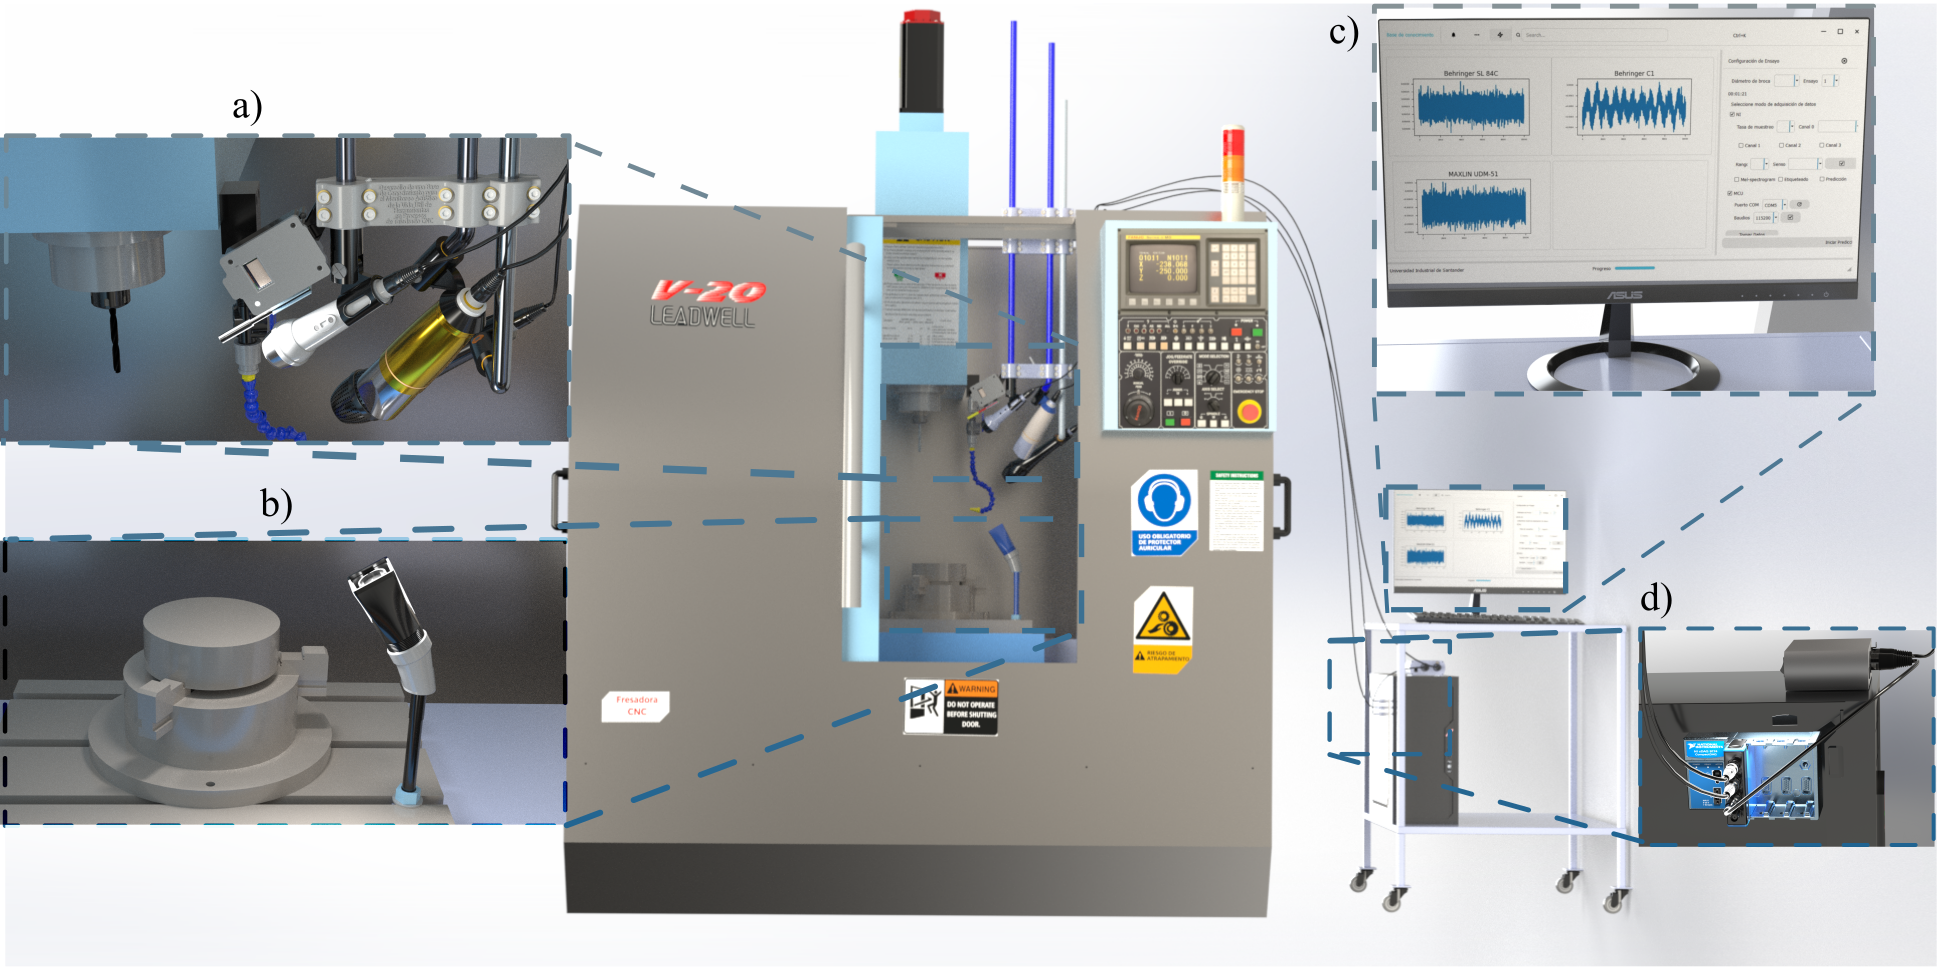
\includegraphics[width=0.85\textwidth]{figures/sistema_completo_v20.png}
\caption{Vista general del sistema de instrumentación completo instalado en el centro de mecanizado Leadwell V-20: arreglo de micrófonos (guía EMT + abrazaderas), case ESP32 con caudalímetro YF-S201 y módulo NI cDAQ-9174.}
\end{figure}

Además del arreglo acústico, el sistema requiere subsistemas complementarios (cámara y caudalímetro) cuya integración mecánica debe garantizar sincronía posicional y protección contra refrigerante; a continuación, se describen esos subconjuntos y su interfaz mecánica con la máquina.

\subsection{Montaje de subsistema de cámara}

El subsistema de cámara microscópica se integra como tercer canal de evidencia del ensayo, complementando a la cadena acústica y al registro de caudal. Su función es documentar la evolución geométrica del filo en las paradas programadas por la rutina de taladrado y proporcionar la etiqueta de desgaste visual a lo largo de la vida útil de cada broca. El conjunto se monta sobre un soporte articulado instalado en el costado de la cabina (Figura~\ref{fig:microscopio-case}), que permite enfocar el flanco de la broca cuando el husillo se posiciona en el punto de inspección. Para evitar que el condensado de taladrina empañara la óptica durante los ciclos largos, la cámara se alojó en un \emph{case} ventilado diseñado \textit{ad hoc} que mantiene el objetivo seco sin interferir con el recorrido del cabezal; esta mejora fue necesaria tras detectar, en las sesiones preliminares, que la humedad ambiental dentro de la cabina degradaba las imágenes de inspección.

\begin{figure}[htbp]
\centering
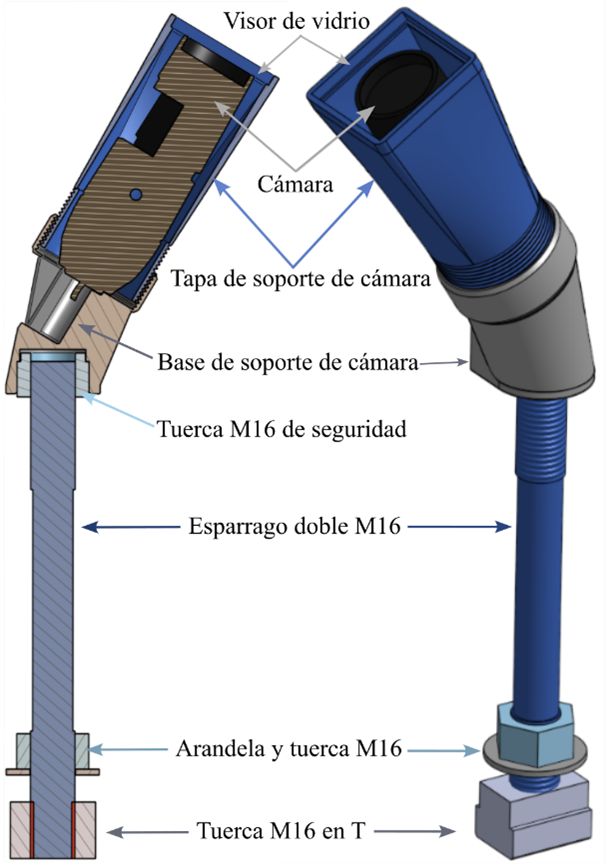
\includegraphics[width=0.70\textwidth,keepaspectratio]{figures/microscopio_case_antiempanamiento.png}
\caption[C\'{a}mara microsc\'{o}pica con carcasa antiempa\~{n}amiento]{C\'{a}mara microsc\'{o}pica CMOS alojada en la carcasa de protecci\'{o}n dise\~{n}ada para evitar el empa\~{n}amiento del objetivo por la taladrina vaporizada. El soporte articulado permite enfocar el flanco de la broca en cada parada programada.}
\label{fig:microscopio-case}
\end{figure}

\subsection{Montaje de subsistema de caudalímetro y case módulo ESP32}

Dada la selección del sensor de caudal, se establece la necesidad de seleccionar accesorios de tubería entre la válvula de bola de 3/8” y la boquilla de salida final por donde se entrega la taladrina a la interfaz herramienta viruta como se muestra en la figura. El montaje electromecánico del nodo ESP32 se completa con un \emph{case} impreso en ABS que aloja la placa, la microSD, la pantalla OLED de monitoreo y el caudalímetro YF-S201; el conjunto se etiqueta y protege para operar de forma continua en el entorno de taladrado (Figura~\ref{fig:esp32-case-caudalimetro}).

\begin{figure}[htbp]
\centering
\begin{minipage}{0.48\textwidth}\centering
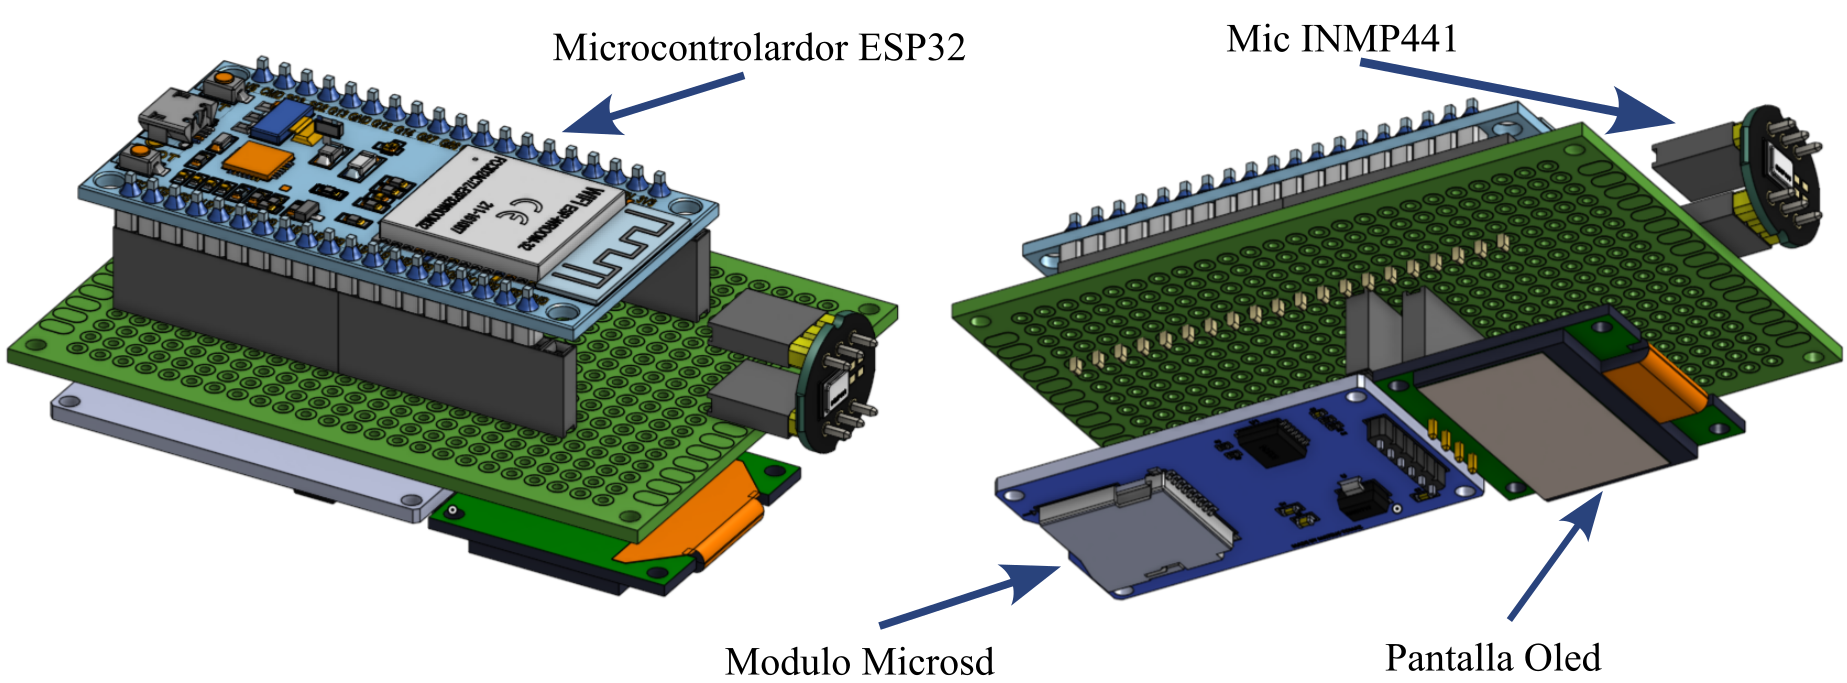
\includegraphics[width=\textwidth,keepaspectratio]{figures/prototipo_case_esp32.png}\\
\small (a) Prototipo inicial del case ESP32.
\end{minipage}\hfill
\begin{minipage}{0.48\textwidth}\centering
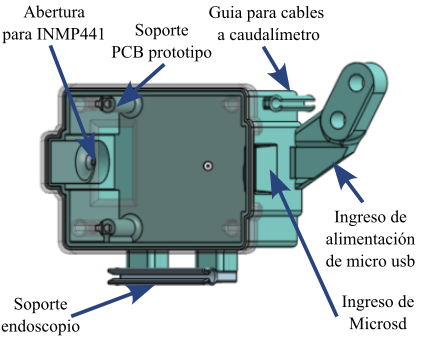
\includegraphics[width=\textwidth,keepaspectratio]{figures/case_esp32_etiquetado.png}\\
\small (b) Versi\'{o}n final etiquetada en servicio.
\end{minipage}
\caption[Case de protecci\'{o}n del m\'{o}dulo ESP32]{Evoluci\'{o}n del \textit{case} del nodo ESP32: (a)~prototipo inicial con electr\'{o}nica expuesta para validaci\'{o}n r\'{a}pida y (b)~versi\'{o}n final con etiquetado de pines, gu\'{i}a de cableado para la alimentaci\'{o}n y la microSD, y ventanas de acceso a los conectores del caudal\'{i}metro.}
\label{fig:esp32-case-caudalimetro}
\end{figure}

\begin{figure}[htbp]
\centering
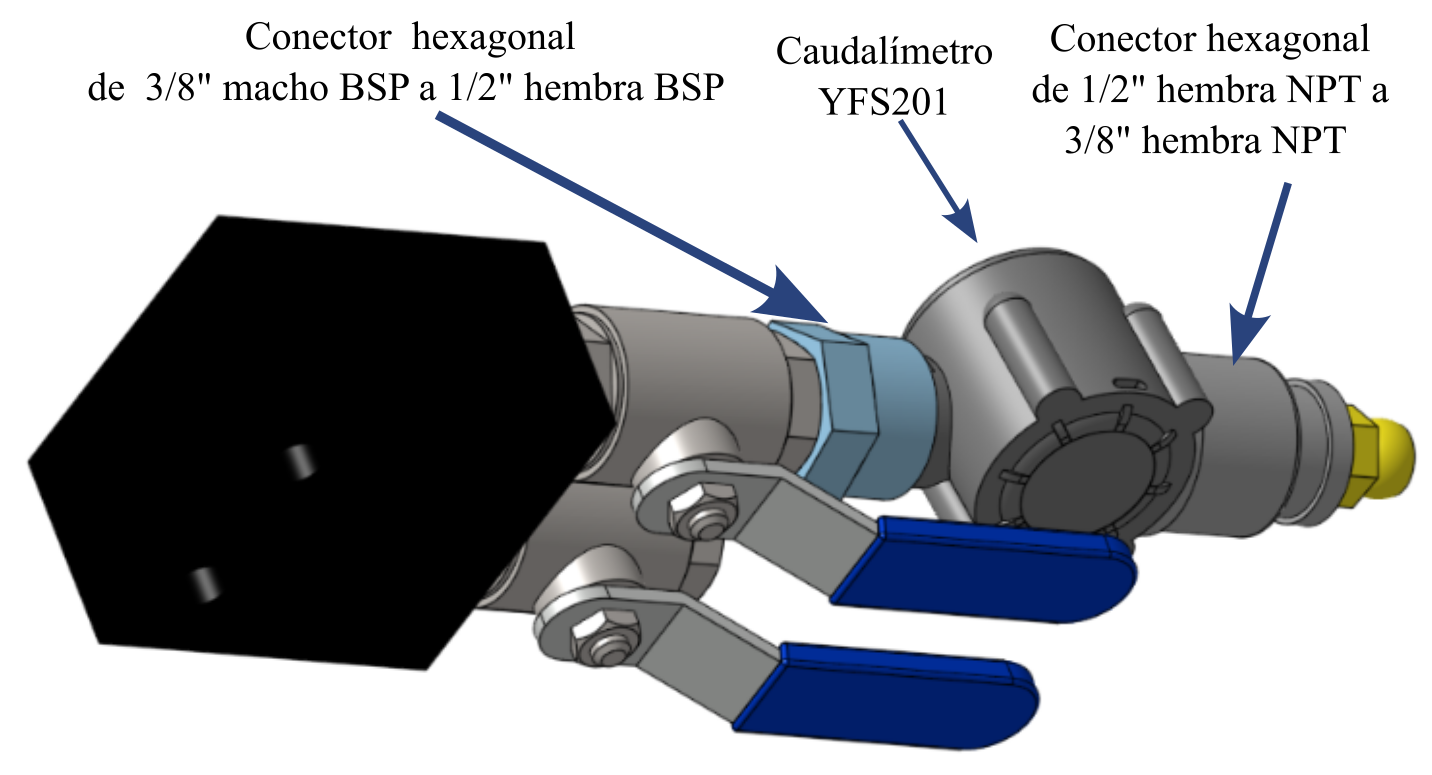
\includegraphics[width=0.55\textwidth,keepaspectratio]{figures/caudalimetro_yfs201.png}
\caption[Caudal\'{i}metro YF-S201]{Caudal\'{i}metro de efecto Hall YF-S201 montado en serie con la l\'{i}nea de taladrina; el sensor genera un tren de pulsos proporcional al flujo volum\'{e}trico que el ESP32 registra con marcas de tiempo sincronizadas con la cadena NI.}
\label{fig:caudalimetro-yfs201}
\end{figure}

\begin{figure}[htbp]
\centering
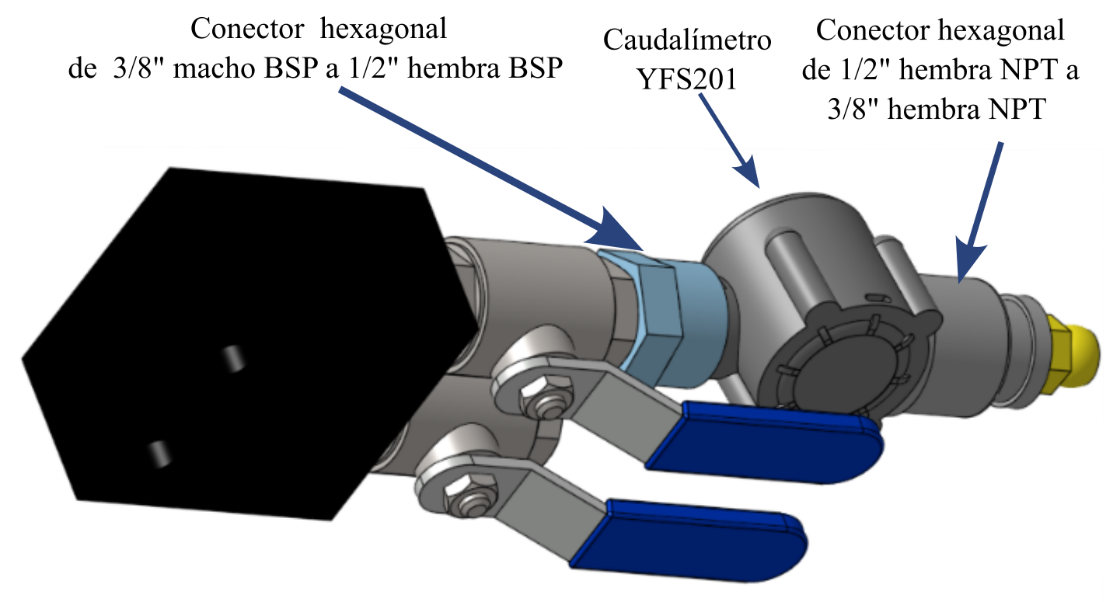
\includegraphics[width=0.65\textwidth,keepaspectratio]{figures/img_024.png}
\caption{Accesorios de tuber\'{i}a para la l\'{i}nea de refrigerante y montaje del caudal\'{i}metro YF-S201 del prototipo electr\'{o}nico ESP32.}
\end{figure}

\begin{figure}[htbp]
\centering
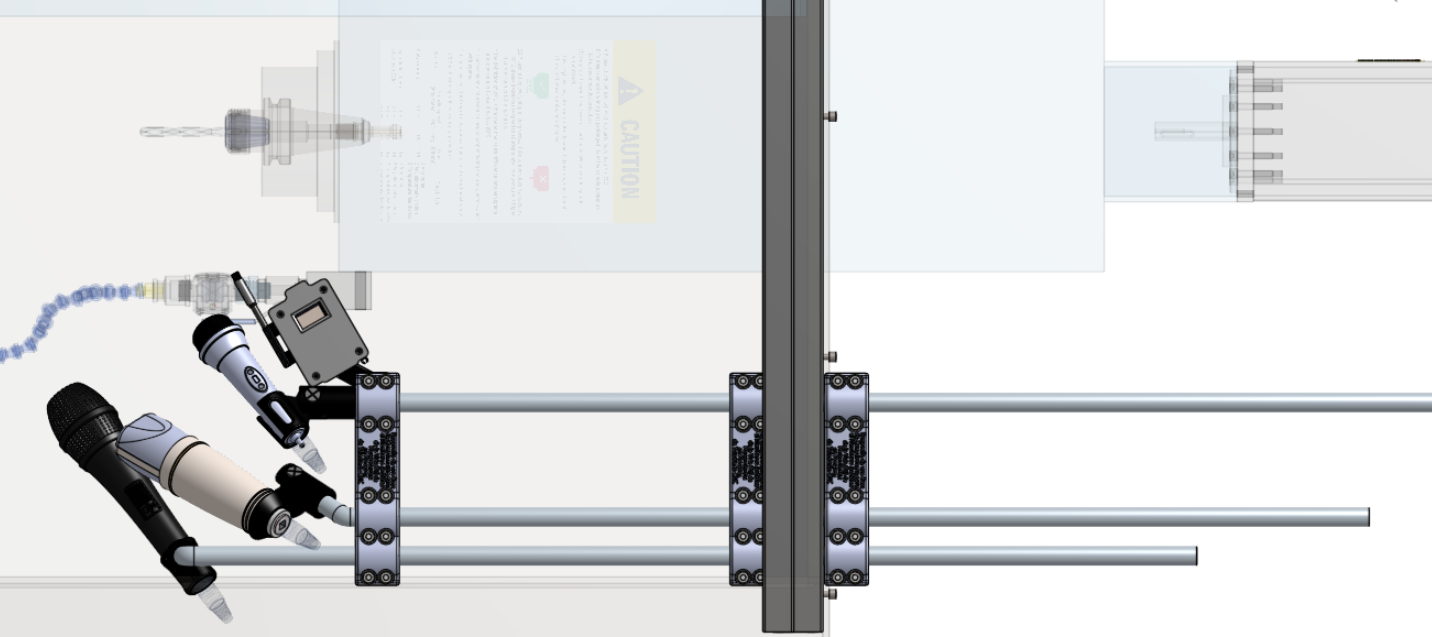
\includegraphics[width=0.85\textwidth]{figures/img_023.png}
\caption{Vista lateral del sistema de sensores del Lote~II con el arreglo de micr\'{o}fonos sobre gu\'{i}a EMT instalado en la pared acrílica del Leadwell V-20.}
\end{figure}

Con los subconjuntos definidos (micrófonos, cámara, caudalímetro) se proponen tres opciones de montaje global (Alternativa A, B y C). Cada alternativa será evaluada según criterios operacionales y experimentales: reproducibilidad posicional, impacto en la transmisión vibratoria, facilidad de instalación (y reversibilidad), protección frente a refrigerante, coste y compatibilidad con la operativa del Leadwell V-20. La selección final se explica al cierre de la sección, justificando la decisión técnica frente a los objetivos experimentales.

\subsection{Alternativa A}

En lugar de diseñar piezas nuevas o alterar la arquitectura principal del equipo, esta alternativa aprovecha los elementos comunes ya existentes y no críticos del chasis para integrar el conjunto de micrófonos. La idea es sencilla y elegante: usar la tornillería y las estructuras del bastidor como puntos de anclaje, evitando cualquier intervención en la geometría esencial de la máquina. (Ver Figura 17. Alternativa A.)



La propuesta concreta consiste en sustituir cuatro tornillos no críticos del conjunto guía de la puerta y del chasis superior por tornillos de mayor longitud que actúen como pernos de fijación para los soportes del sistema de micrófonos. Con este cambio, los soportes quedan sujetos de forma rígida y reproducible, sin tocar piezas estructurales esenciales ni interferir con los recorridos o zonas de trabajo del cabezal. El montaje es no invasivo y reversible: se preservan los tornillos originales y se documenta el procedimiento en el protocolo de ensayo para poder restaurar la configuración inicial en cualquier momento. 

Este enfoque aporta varias ventajas prácticas: es una solución de bajo coste que aprovecha anclajes ya existentes, facilita una instalación rápida y su reversibilidad reduce al mínimo los riesgos operativos y el tiempo de paro de la máquina. No obstante, conviene ser prudente: antes de ejecutar el cambio hay que verificar que los tornillos a sustituir sean realmente no críticos y que su reemplazo no afecte la estanqueidad ni el ajuste de las guías. Además, aunque la solución ofrece suficiente estabilidad para los objetivos experimentales planteados, puede no proporcionar la misma libertad posicional que un soporte externo hecho a medida ---algo a valorar según las necesidades futuras de posicionamiento y accesibilidad.

En resumen, Alternativa A es una intervención práctica, documentable y fácilmente reversible que maximiza el uso de la infraestructura existente para añadir el sistema de micrófonos con mínima intrusión y riesgo, siempre acompañada de las comprobaciones necesarias sobre la criticidad de los puntos de anclaje.

\subsection{Alternativa B}

La Alternativa B plantea desacoplar completamente la instrumentación acústica del chasis del centro de mecanizado mediante el uso de caballetes independientes dispuestos transversalmente al eje de trabajo. Cada caballete sostiene su propio subconjunto de micrófono, electrónica y canalizaciones, de modo que se elimina el contacto directo con la estructura de la máquina y se reduce la vía de transmisión de vibraciones estructurales hacia la señal acústica.

\begin{figure}[htbp]
\centering
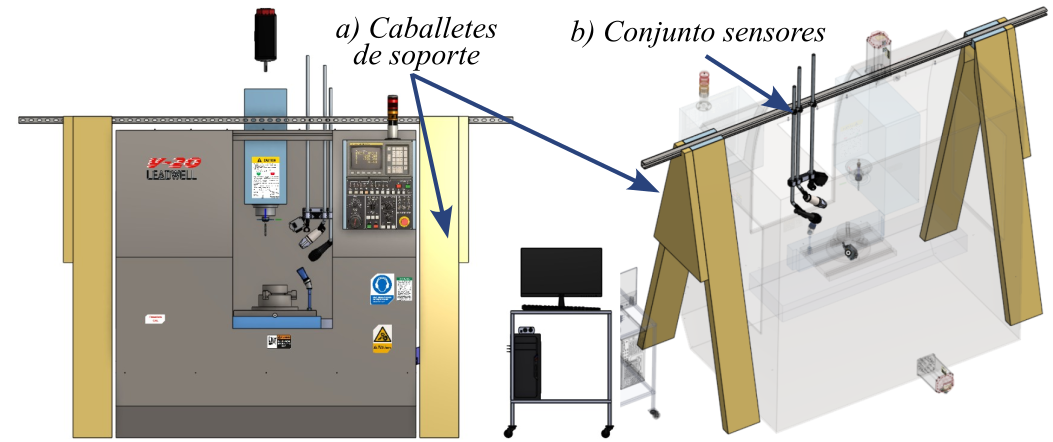
\includegraphics[width=0.75\textwidth,keepaspectratio]{figures/img_027.png}
\caption{Alternativa B: soporte de instrumentaci\'{o}n sobre caballetes independientes desacoplados del chasis del centro de mecanizado.}
\end{figure}

Los caballetes se constituyen como estructuras rígidas de perfil de acero (sección rectangular o perfil en U) con refuerzos triangulados para asegurar rigidez frente a la flexión. En la base se incorpora una interfaz antivibratoria ---mediante pads de neopreno o Sorbothane, o monturas roscadas antivibración--- que atenúa las bandas bajas y medias en las que la máquina concentra su energía mecánica. En la parte superior se dispone una plataforma regulable: una placa con tornillería y espaciadores que permite ajustar altura e inclinación para alinear el micrófono respecto al husillo. El porta-micrófono se fija con elementos rígidos cuando se prioriza la repetibilidad, admitiendo desacoples elásticos cuando se requiere suavizar la transmisión residual. El cableado se conduce por canalizaciones protegidas con sujetacables, \textit{drip loops} y puntos de anclaje que eliminan la tracción y el ruido por microfonía.

El fundamento físico de esta alternativa radica en la separación de masas: al aislar la masa de la instrumentación respecto a la masa de la máquina se reduce la transferencia directa de vibraciones, obteniendo una señal acústica con mejor relación señal-ruido en las bandas bajas dominadas por la maquinaria. Desde el punto de vista del análisis de datos, este desacoplo disminuye la correlación espuria entre vibraciones estructurales y eventos acústicos reales de corte, favoreciendo que los modelos aprendan características del contacto herramienta-pieza y no artefactos del bastidor.

Entre las ventajas de esta configuración se destacan el aislamiento superior frente a vibraciones, la posibilidad de ajuste fino de la posición y orientación de cada micrófono, y una instalación no invasiva que no requiere modificar tornillería ni paneles de la máquina. No obstante, la alternativa presenta limitaciones relevantes: requiere mayor espacio en el área de trabajo y una base de apoyo estable, lo que la hace poco viable en laboratorios reducidos; y si los aisladores o la geometría del soporte no se dimensionan adecuadamente, la propia estructura puede introducir resonancias que coloreen la señal. Por ello resulta crítico diseñar la rigidez y la masa del conjunto de modo que las frecuencias naturales queden fuera de la banda de interés.

Adicionalmente, la independencia respecto a la máquina introduce consideraciones operativas: puede complicar la sincronización posicional cuando el centro de mecanizado requiere movimientos o accesos que interfieran con los caballetes, estableciendo un compromiso entre aislamiento vibratorio y ocupación física del espacio de trabajo que debe evaluarse según la normativa del laboratorio y la naturaleza de los ensayos previstos.

En síntesis, la Alternativa B maximiza el aislamiento vibratorio y la calidad de la señal acústica, pero implica mayor ocupación espacial y riesgo de resonancias derivadas de la propia estructura de soporte.

\subsection{Alternativa C}

Esta alternativa propone introducir el subconjunto de micrófonos en sentido horizontal a través de la ventana acrílica de la máquina. Para ello se realizarán tres pasos pasantes en el panel acrílico, por donde se desplazarán los conductos EMT que sirven de guía y soporte del arreglo micrófonico. Cada conducto EMT tendrá longitud suficiente para apoyarse sobre el chasis exterior de la máquina y alojar las abrazaderas que fijan los micrófonos. En el interior de la cabina, las abrazaderas sujetarán el conjunto sobre la cara interna del acrílico; en el exterior el EMT apoyará y se atornillará al chasis usando puntos de anclaje no críticos, de forma que la modificación sea reversible y no altere estructuras funcionales del equipo (ver detalle en Figura 19. \textit{Detalle de ensamblaje de la alternativa C}).

Ventajas principales:

\begin{itemize}[leftmargin=1.77cm]
\item Montaje compacto y reproducible: permite posicionar micrófonos en puntos definidos y replicables entre ensayos.
\item Protección física y sellado: uso de prensaestopas y juntas evita ingreso de refrigerante y protege el cableado.
\item Facilidad para calibrar y reubicar: el sistema EMT + abrazaderas facilita ajustes posicionales sin necesidad de nuevos mecanizados. 
\end{itemize}


\begin{figure}[htbp]
\centering
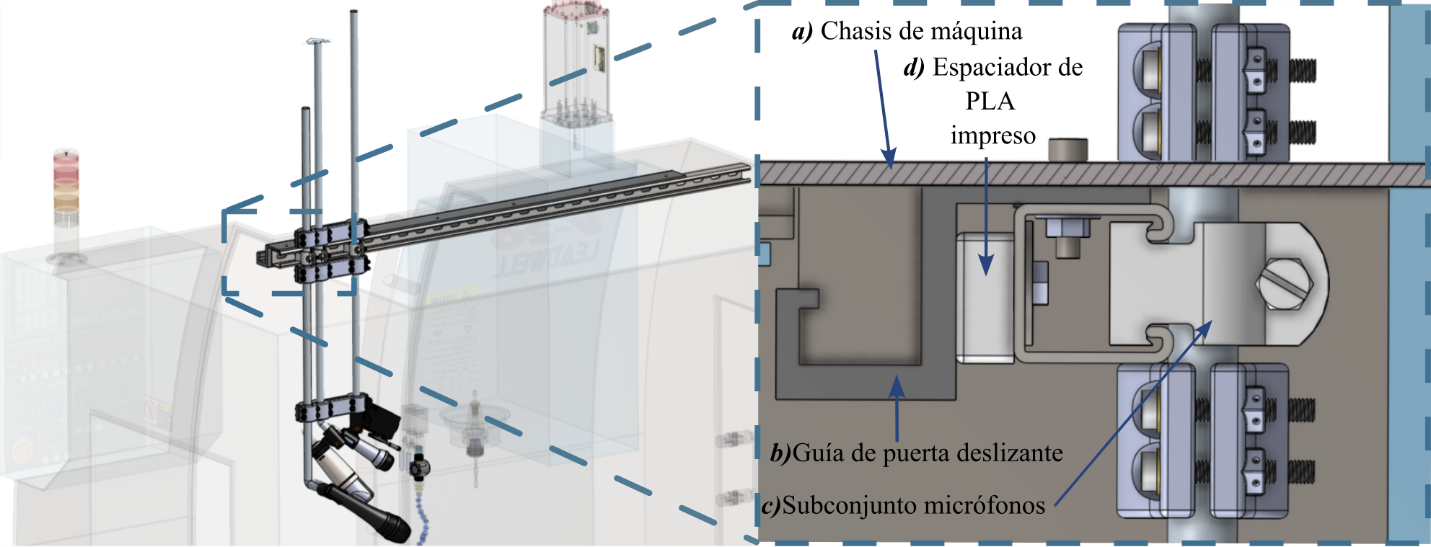
\includegraphics[width=0.85\textwidth]{figures/img_026.png}
\caption{Detalle de ensamblaje de la Alternativa C: conducci\'{o}n del arreglo de micr\'{o}fonos a trav\'{e}s de pasos pasantes en el panel acr\'{i}lico de la m\'{a}quina.}
\end{figure}

\subsection{Tipo de montaje seleccionado}

Se evaluaron tres alternativas generales (A, B y C) según criterios operacionales y experimentales: reproducibilidad posicional, impacto en transmisión vibratoria, facilidad de instalación y reversibilidad, protección frente a refrigerante, coste y compatibilidad con la operativa del Leadwell V-20. Tras la evaluación práctica y el balance de riesgos/beneficios, se selecciona la Alternativa A como montaje definitivo para la ejecución de los ensayos piloto y la generación de la base de conocimiento.

Alternativa A --- montaje sobre tornillería y anclajes existentes

La solución consiste en reutilizar anclajes no críticos del chasis y la guía de la puerta: se sustituyen cuatro tornillos seleccionados por tornillos de mayor longitud que actúan como puntos de fijación para los soportes del sistema de micrófonos. Con ello se consigue fijación rígida, replicable y reversible sin modificar la geometría funcional de la máquina.

Ventajas con la selección:

\begin{itemize}[leftmargin=1.77cm]
\item Instalación rápida, económica y reversible por tanto no requiere estructuras externas ni obras en el taller.
\item Minimiza tiempos de parada y riesgo de dañar la máquina, facilitando la aprobación operativa por parte del laboratorio/taller.
\item Proporciona rigidez suficiente para mantener coordenadas posicionales estables entre ensayos, lo que es crítico para trazabilidad y para evitar sesgos posicionales en los modelos.
\end{itemize}
Limitaciones y mitigaciones propuestas:

\begin{itemize}[leftmargin=1.77cm]
\item Una limitación detectada es disminución de aislamiento ante vibraciones que ofrece un caballete desacoplado (Alternativa B).
\item Mitigación pasiva y activa: Conjunto de abrazaderas plásticas que sujetan las tres tuberías en tres puntos, con una manga termo-retráctil colocada entre tubería y abrazadera. Esta solución reduce la transmisión de vibraciones mecánicas y, al introducir una superficie rugosa/plástica en el contacto, aumenta la fricción evitando el deslizamiento metal-sobre-metal. Como complemento físico se aplican contramedidas en el procesamiento de señal (filtrado digital: notch / band-stop, pasa-altas; y técnicas de separación de fuentes) para atenuar remanentes de ruido estructural durante el preprocesado.
\end{itemize}


Con el montaje mecánico definido y documentado, el capítulo 5 detalla la integración electrónica (NI Cdaq 9174, NI-9234, nodos ESP32), la arquitectura del software de adquisición y las funciones necesarias para garantizar sincronización, muestreo consistente, captura de video en paradas programadas y la actualización automática del manifiesto. En particular, el capítulo 5 presenta los procedimientos de verificación automática (SNR, checksums, duración) que complementan los checklist manuales aquí descritos.

\clearpage
\chapter{Sistema de adquisición de datos}

El sistema de adquisición diseñado captura de forma sincronizada señales acústicas multicanal, video (inspección del filo) y caudal de refrigerante para generar una base de conocimiento multimodal sobre el desgaste de brocas en taladrado CNC. Sus objetivos principales son: (i) preservar la máxima fidelidad de las señales de referencia, (ii) permitir una monitorización en tiempo real de la salud de los sensores e integridad de los datos, y (iii) asegurar trazabilidad y reproducibilidad mediante un manifiesto de metadatos. La solución integra dos cadenas de adquisición complementarias: una referencia de alta fidelidad basada en National Instruments (NI) y un piloto económico basado en nodos ESP32+INMP441.

A continuación, se resume la arquitectura y las decisiones de diseño adoptadas para cada subcomponente del sistema.

\section{Sensores}

El micrófono es el transductor responsable de cuantificar el fenómeno físico ya que transforma las vibraciones producidas por la presión acústica sobre su cápsula en una señal eléctrica. Por ello constituye el elemento más crítico del sistema de adquisición acústica y su selección condiciona directamente la fidelidad de los datos recogidos.

Para este ensayo se eligieron tres micrófonos con características complementarias que responden a los requisitos definidos: patrón polar direccional (cardioide), respuesta amplia y relativamente plana en frecuencia, y robustez operativa en entorno industrial. A continuación, se describen sus propiedades y el papel que cumplen en el montaje experimental:

\begin{table}[htbp]
\centering
\caption{\textit{Características técnicas del micrófono 1: Behringer C1 (condensador).}}
\label{tab:mic-c1}
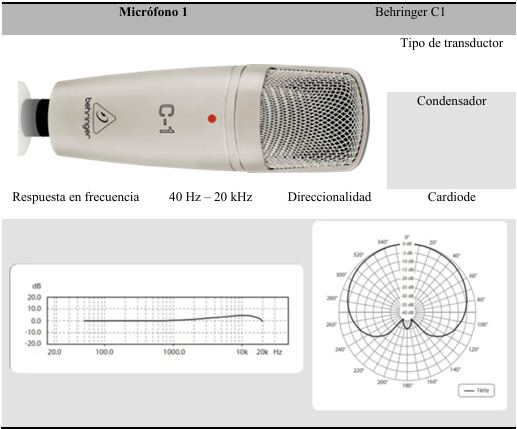
\includegraphics[width=0.85\textwidth]{figures/tabla_06.png}
\end{table}

El micrófono condensador Behringer C1 (Tabla~\ref{tab:mic-c1}) ofrece alta sensibilidad y respuesta en frecuencia extendida y lineal, lo que favorece la captura de componentes espectrales finos que anticipan fases de desgaste incipiente. Su patrón polar cardioide reduce la captación de reflexiones laterales en el entorno de mecanizado. Requiere alimentación \textit{phantom} de 48~V suministrada por el módulo NI-9234.

\begin{table}[htbp]
\centering
\caption{\textit{Características técnicas del micrófono 2: Behringer SL 84C (dinámico).}}
\label{tab:mic-sl84c}
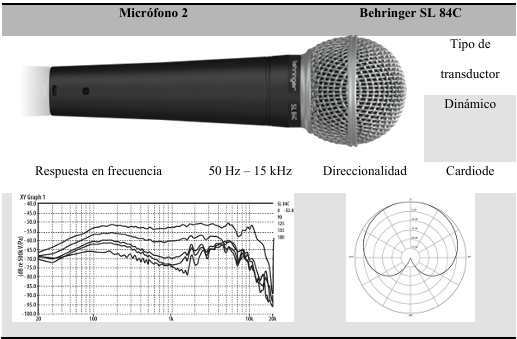
\includegraphics[width=0.85\textwidth]{figures/tabla_07.png}
\end{table}

El Behringer SL~84C (Tabla~\ref{tab:mic-sl84c}) es un micrófono dinámico que, por su construcción pasiva, tolera condiciones adversas de temperatura, humedad y salpicaduras propias del entorno de taladrado. Su menor sensibilidad respecto al condensador se compensa con la robustez operativa y la nula susceptibilidad a picos de presión acústica.

\begin{table}[htbp]
\centering
\caption{\textit{Características técnicas del micrófono 3: MAXLIN UDM-51 (dinámico).}}
\label{tab:mic-udm51}
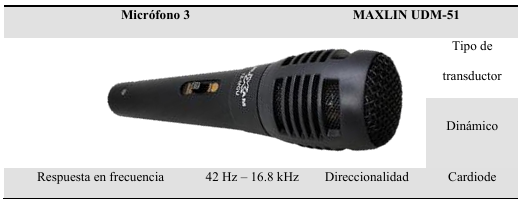
\includegraphics[width=0.85\textwidth]{figures/tabla_08.png}
\end{table}

El MAXLIN UDM-51 (Tabla~\ref{tab:mic-udm51}) es un micrófono dinámico de bajo costo que combina robustez mecánica con una respuesta suficiente para cubrir el rango de frecuencias relevante en el taladrado CNC. Su inclusión en el sistema permite aumentar la redundancia de canal y diversificar la sensibilidad espectral del conjunto.

\subsection{Comparación y uso conjunto en el experimento}

\subsubsection{Complementariedad}

La combinación de un condensador (C-1) y dos dinámicos (SL84C, UDM-51) aporta un buen balance entre sensibilidad (detección de componentes débiles y armónicos con el C-1) y robustez operacional (resistencia a condiciones adversas con los dinámicos). Esto facilita la construcción de modelos que sean a la vez sensibles y generalizables.

\subsubsection{Phantom y preamplificación}

Dado que el C-1 necesita phantom, la cadena de adquisición debe contemplar alimentación phantom y/o un preamplificador con entradas XLR balanceadas. Evitar alimentar micrófonos phantom de forma inadecuada (p. ej. mediante adaptadores improvisados) para no dañar cápsulas o electrónica.

\subsubsection{Montaje y posicionamiento}

 Todos los micrófonos se montan con soportes rígidos de micrófono que garanticen la geometría posicional documentada en el manifiesto y a su vez se asegura que cada componente electrónico expuesto se cubra con termo-encogible de la dimensión apropiada para la geometría tanto del terminal XLR hembra del cable como del terminal macho del micrófono. Se recomienda usar amortiguadores mecánicos y elementos de fijación que eviten contacto rígido directo con superficies que transmitan vibraciones estructurales.

\subsection{Ubicación de los sensores}

La ubicación de los tres micrófonos se definió según los criterios de posicionamiento descritos en la sección de montaje mecánico (Sección~3.1.1). Las coordenadas exactas de cada sensor se registran en el manifiesto de cada sesión experimental y se documentan fotográficamente como parte del protocolo de trazabilidad.

\begin{figure}[htbp]
\centering
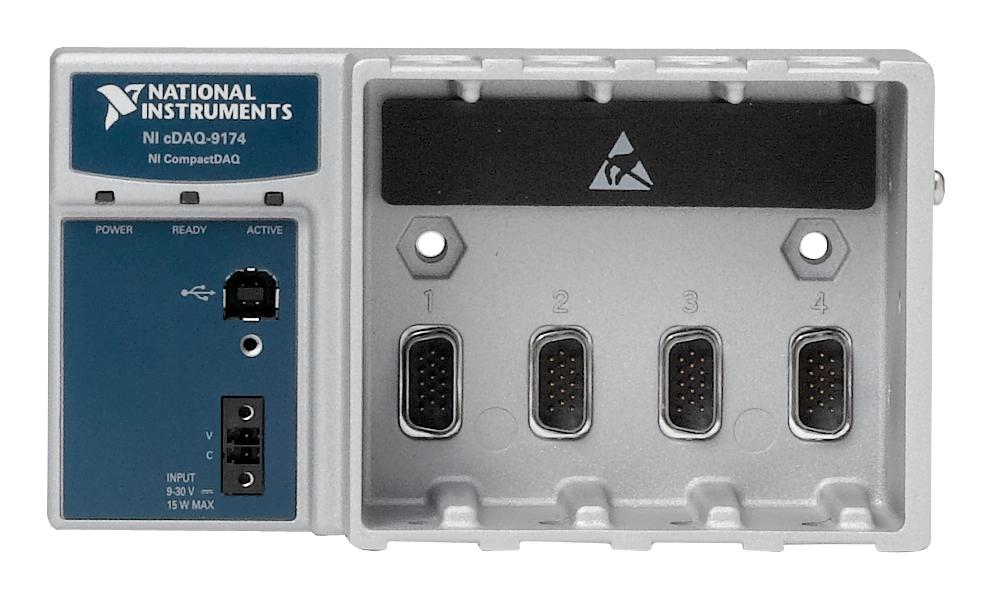
\includegraphics[width=0.55\textwidth,keepaspectratio]{figures/img_038.jpg}
\caption[Chasis NI cDAQ-9174]{Módulo NI cDAQ-9174: chasis de adquisici\'{o}n USB de cuatro ranuras para módulos de la serie C de National Instruments.}
\label{fig:ni-cdaq9174}
\end{figure}

\subsection{Pruebas preliminares: comportamiento ante saturación del ADC}
\label{subsec:pruebas-microfono-saturacion}

Durante las pruebas preliminares de los tres micrófonos se verificó
sistemáticamente el rango dinámico útil de cada cadena de adquisición
frente al proceso de taladrado. El micrófono condensador (Behringer C1)
exhibe la mayor sensibilidad, lo que introduce riesgo de saturación del
conversor analógico--digital (ADC) del módulo NI-9234 cuando la
herramienta atraviesa transitorios energéticos --entrada de broca,
cambios abruptos de régimen de corte o fracturas incipientes--. Los
micrófonos dinámicos (Behringer SL84C y MAXLIN UDM-51), en cambio,
toleran presiones sonoras más elevadas sin comprometer el rango útil.

Como consecuencia operativa de estas pruebas se definió una regla de
protección del canal de referencia: cuando el canal del condensador
registra picos que alcanzan el fondo de escala del ADC, la segmentación
automática de agujeros conmuta a una estrategia de respaldo
(\textit{fallback}) basada en el valor cuadrático medio
(\textit{RMS}, \textit{root-mean-square}) del canal dinámico, que
preserva la envolvente de energía aunque la información espectral fina
quede parcialmente comprometida. Esta decisión se recoge como marca
\texttt{is\_saturated} en los metadatos del manifiesto y condiciona el
pipeline de segmentación descrito en el
Capítulo~\ref{cap:procesamiento-actual}.

\section{Hardware de adquisición}

\noindent El sistema de adquisición de datos se diseñó teniendo en cuenta la necesidad de capturar señales acústicas, imágenes y variables auxiliares de forma sincronizada y confiable. Para esto, se mantuvo la plataforma principal empleada por Orejarena \& Peña (2014), compuesta por un chasis NI cDAQ-9174 y un módulo NI-9234, a la cual se integraron nuevos componentes desarrollados en este proyecto, incluyendo un sistema auxiliar basado en ESP32 y una cámara microscópica CMOS.

\noindent Esta integración permitió ampliar la capacidad de adquisición y garantizar que todas las señales relevantes se registraran de forma simultánea para su análisis posterior.

\subsection{Sistema principal NI}

La solución de adquisición centraliza la captura de señales críticas en el chasis modular de NI, decisión que se mantiene por su robustez y capacidad para manejar mediciones acústicas y vibratorias de alta precisión. Este enfoque prioriza la fiabilidad en la captura, la adecuada cobertura en frecuencia para registrar transitorios del proceso de corte, y la resolución necesaria para distinguir cambios sutiles en la dinámica de las señales. El chasis utilizado ---NI cDAQ-9174 (chasis cDAQ-9174)--- aporta una plataforma compacta de cuatro ranuras y comunicación por USB, que simplifica la integración con el computador de control y facilita la sincronización entre módulos y la generación de marcas temporales (timestamps) consistentes entre canales.


\begin{figure}[htbp]
\centering
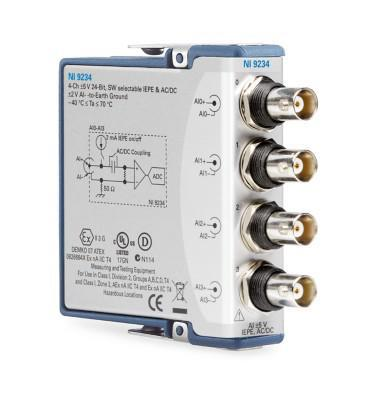
\includegraphics[width=0.38\textwidth,keepaspectratio]{figures/img_039.jpg}
\caption[Módulo NI-9234]{M\'{o}dulo NI-9234 de cuatro canales (51{,}2~kS/s, 24~bits, acoplamiento AC, IEPE) instalado en el chasis cDAQ-9174 para la adquisici\'{o}n de se\~{n}ales ac\'{u}sticas de alta fidelidad.}
\label{fig:ni-9234}
\end{figure}

Dentro del chasis se instala el módulo optimizado para señales acústicas: el NI-9234 (módulo NI-9234). Este módulo combina muestreo de alta velocidad y alta resolución ---hasta 51.2 kS/s por canal y 24 bits de resolución--- con filtros anti-aliasing integrados y entradas compatibles con micrófonos IEPE o señales condicionadas a través de preamplificadores. En la práctica se explotan tres canales paralelos de captura para micrófonos de alta fidelidad, lo que mejora la cobertura espacial de la emisión acústica y atenúa sesgos instrumentales al permitir análisis multicanal y técnicas de fusión espacial. La arquitectura NI facilita además la adquisición síncrona de canales analógicos y digitales, requisito para alinear audio, triggers y eventos de parada programada para inspección visual.

\subsection{Sistema auxiliar ESP32}

Como complemento económico y flexible a la plataforma NI, se integra un subsistema basado en la placa ESP32. Este nodo auxiliar se dedica a registrar variables complementarias en tiempo real, útiles para enriquecer el dataset y para validaciones rápidas. Entre sus sensores se incluyen un caudalímetro YF-S201 (YF-S201 flowmeter), que convierte el flujo de taladrina en pulsos medibles y permite seguir la estabilidad del refrigerante a lo largo de cada ensayo; y un micrófono digital INMP441 (INMP441, interfaz I$^2$S), que ofrece una alternativa de captura de audio con respuesta hasta \textasciitilde{}16 kHz para prototipos, pruebas de verificación y como respaldo frente a fallas puntuales del sistema principal.


\begin{figure}[htbp]
\centering
\begin{minipage}{0.58\textwidth}\centering
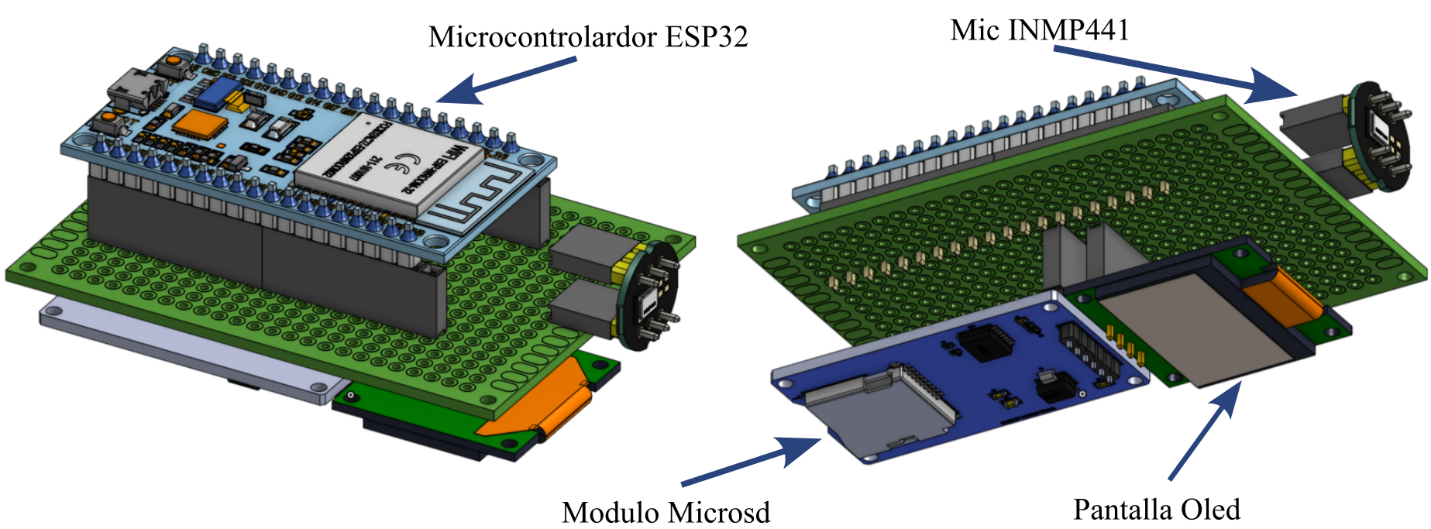
\includegraphics[width=\textwidth,keepaspectratio]{figures/img_040.png}\\
\small (a) M\'{o}dulo ESP32 + INMP441 + YF-S201.
\end{minipage}\hfill
\begin{minipage}{0.38\textwidth}\centering
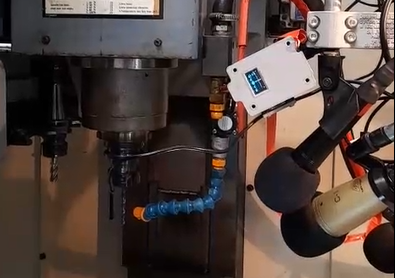
\includegraphics[width=\textwidth,keepaspectratio]{figures/esp32_instalado_maquina.png}\\
\small (b) Nodo instalado sobre el Leadwell V-20.
\end{minipage}
\caption[M\'{o}dulo ESP32 y su instalaci\'{o}n en m\'{a}quina]{(a)~M\'{o}dulo de adquisici\'{o}n ESP32 con micr\'{o}fono MEMS INMP441, pantalla OLED y sensor de caudal YF-S201 integrados en el case de protecci\'{o}n. (b)~Nodo montado sobre el Leadwell V-20 durante una sesi\'{o}n de adquisici\'{o}n: se observa el INMP441 apuntando a la zona de corte y la pantalla OLED graficando el FFT del audio en tiempo real como indicador de salud del canal.}
\label{fig:esp32-modulo}
\end{figure}

La comunicación entre el ESP32 y el sistema de control se realiza mediante un enlace serie o por intercambio de archivos/mensajes con marcas temporales; la sincronización se implementa mediante señales de disparo (trigger) digitales o por timestamping en el software de adquisición, de modo que las series del ESP32 se puedan alinear posteriormente con las trazas de NI y con las paradas de inspección visual. Este arreglo economiza recursos y permite ampliar sensores sin comprometer la adquisición principal.

\subsection{Subsistema de cámara microscópica CMOS}

Para la verificación visual y el etiquetado progresivo del desgaste se incorpora una cámara microscópica basada en sensor CMOS (CMOS microscope camera). Esta cámara captura imágenes de alta resolución del flanco de la broca en las paradas programadas del ciclo de taladrado, y se integra con la misma interfaz de control para garantizar registro sincronizado: cada imagen queda asociada a una marca temporal que permite vincularla con el audio y las lecturas del caudalímetro. Las imágenes cumplen dos funciones complementarias: validación visual del criterio de desgaste (por ejemplo, VB) y generación de etiquetas para modelos supervisados o para estudios de correlación multimodal entre firma acústica y evolución geométrica del filo.

\subsection{Integración y sincronización}

En su conjunto, estos subsistemas forman una arquitectura multicanal y multimodal pensada para capturar señales acústicas de alta calidad junto a variables auxiliares que explican fuentes de variación del proceso. La estrategia práctica combina la robustez del chasis NI para la captura principal, la flexibilidad del ESP32 para sensores complementarios y la evidencia visual proporcionada por la cámara CMOS. Todos los dispositivos se registran en el manifiesto del experimento (manifest), que incluye metadatos por sesión ---identificadores de sensores, configuración de muestreo, torque de apriete, identificación de componentes, y fotografías del montaje--- con el fin de preservar trazabilidad y facilitar procedimientos de control de calidad (QC) y auditoría posterior.

La Figura~\ref{fig:subconjunto-rielmic} documenta el resultado f\'{i}sico del subconjunto de micr\'{o}fonos: el riel EMT con los tres micr\'{o}fonos equidistantes, las abrazaderas amortiguadas y la ruta de cable balanceado hacia el m\'{o}dulo NI-9234. Este subconjunto se valida por separado antes de integrarse al sistema completo y constituye la unidad m\'{i}nima reemplazable del arreglo ac\'{u}stico.

\begin{figure}[htbp]
\centering
\begin{minipage}{0.48\textwidth}\centering
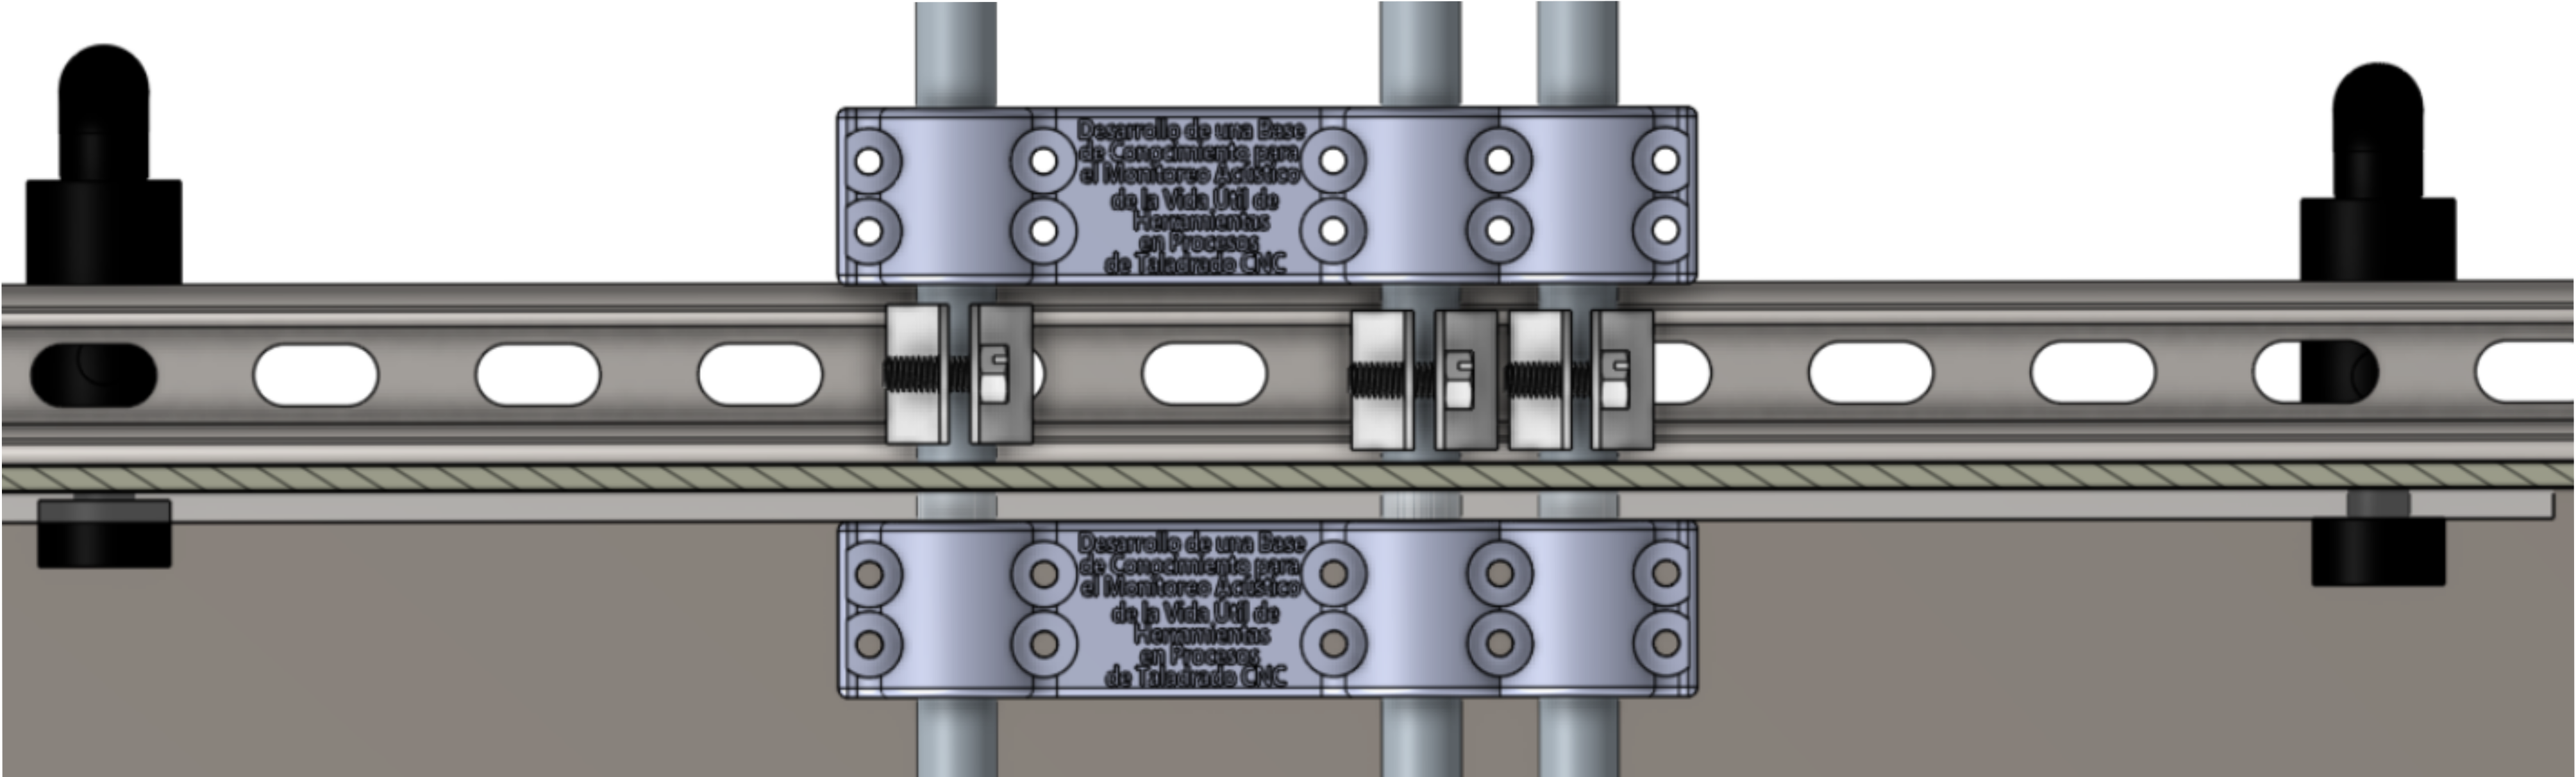
\includegraphics[width=\textwidth,keepaspectratio]{figures/riel_microfonos_detalle.png}\\
\small (a) Detalle del riel con micr\'{o}fonos y abrazaderas.
\end{minipage}\hfill
\begin{minipage}{0.48\textwidth}\centering
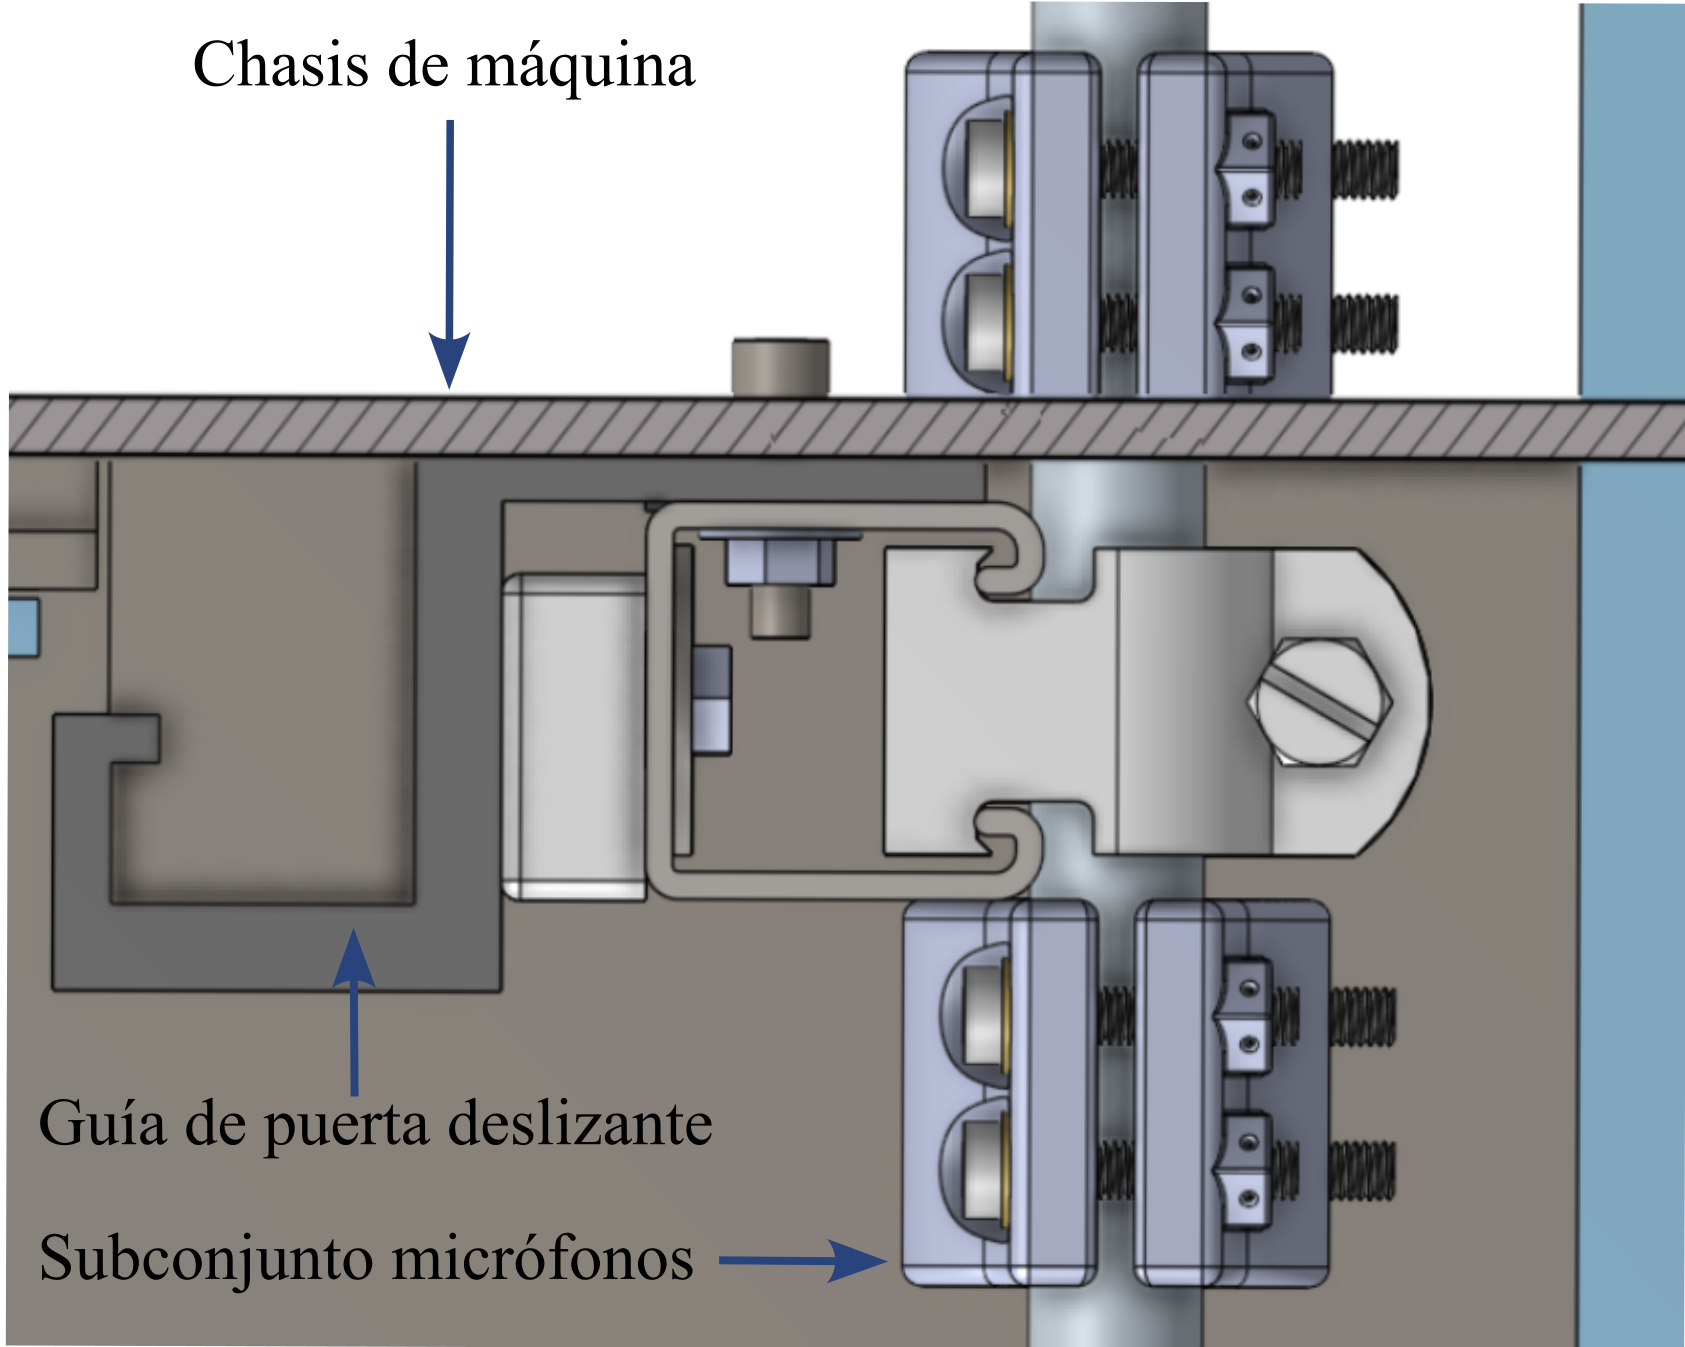
\includegraphics[width=\textwidth,keepaspectratio]{figures/subconjunto_microfonos_puerta.png}\\
\small (b) Subconjunto instalado en la puerta de la cabina.
\end{minipage}
\caption[Subconjunto de micr\'{o}fonos sobre riel EMT]{Subconjunto de micr\'{o}fonos: (a)~detalle del riel EMT con los tres micr\'{o}fonos equidistantes, abrazaderas con manga termo-retr\'{a}ctil y ruta de cableado apantallado; (b)~conjunto instalado sobre la cara interna de la puerta acr\'{i}lica del Leadwell V-20, con pasos pasantes sellados y drip-loops que eliminan la tracci\'{o}n en los conectores XLR.}
\label{fig:subconjunto-rielmic}
\end{figure}

\section{Sistema de conexiones}

La calidad de las conexiones y del cableado constituye una capa crítica del experimento: no solo transporta la señal, sino que condiciona la relación señal/ruido y, por tanto, la capacidad de detectar cambios sutiles asociados al desgaste. En este ensayo se prioriza una solución de cableado diseñada específicamente para aplicaciones de audio de baja amplitud, en lugar de reutilizar cables coaxiales genéricos. La elección y el manejo del cable reducen artefactos eléctricos y mecánicos que de otro modo enmascaran los fenómenos acústicos de interés.


\subsection{Cable de audio seleccionado}

Se utiliza un cable multicapa construido para audio profesional: conductores de cobre sin oxígeno (OFC), aislamiento de polietileno (PE), relleno de fibra textil (algodón), separador de papel, capa conductiva interior (PVC conductor), blindaje en espiral de OFC y cubierta exterior de PVC. Esta arquitectura aporta tres ventajas prácticas para la conexión de los micrófonos al módulo NI-9234:

\begin{itemize}[leftmargin=1.77cm]
\item \textbf{Fidelidad de señales débiles.} La combinación de conductores OFC y aislamiento PE reduce la capacitancia par-a-par, lo que preserva la dinámica y la respuesta en frecuencias que resultan determinantes para características como transitorios, centroides y MFCCs.
\item \textbf{Inmunidad a interferencias.} El blindaje en espiral junto a la capa conductiva actúa como barrera frente a interferencias electromagnéticas (EMI) generadas por motores y variadores del taller; esto disminuye ruidos de banda ancha y pulsos eléctricos que deterioran los análisis espectrales.
\item \textbf{Reducción de artefactos mecánicos.} El relleno interno y la construcción multicapa mitigan la microfonía (ruido por fricción del cable), un problema frecuente en entornos industriales donde el cable se desplaza o choca con soportes.
\end{itemize}
Desde el punto de vista de la instrumentación, el NI-9234 acepta entradas diferenciales y conexiones tipo BNC; por tanto, el cableado se termina con conectores adecuados que preservan la configuración diferencial (evitando bucles de masa no intencionados). Cuando se empleen micrófonos con alimentación IEPE se contemplan transformadores de adaptación o preamplificadores con salida balanceada para explotar la entrada diferencial del módulo NI. La Figura~\ref{fig:xlr-bnc} ilustra el esquema de adaptación entre el conector XLR macho del micrófono y el conector BNC del módulo de adquisición.

\begin{figure}[htbp]
\centering
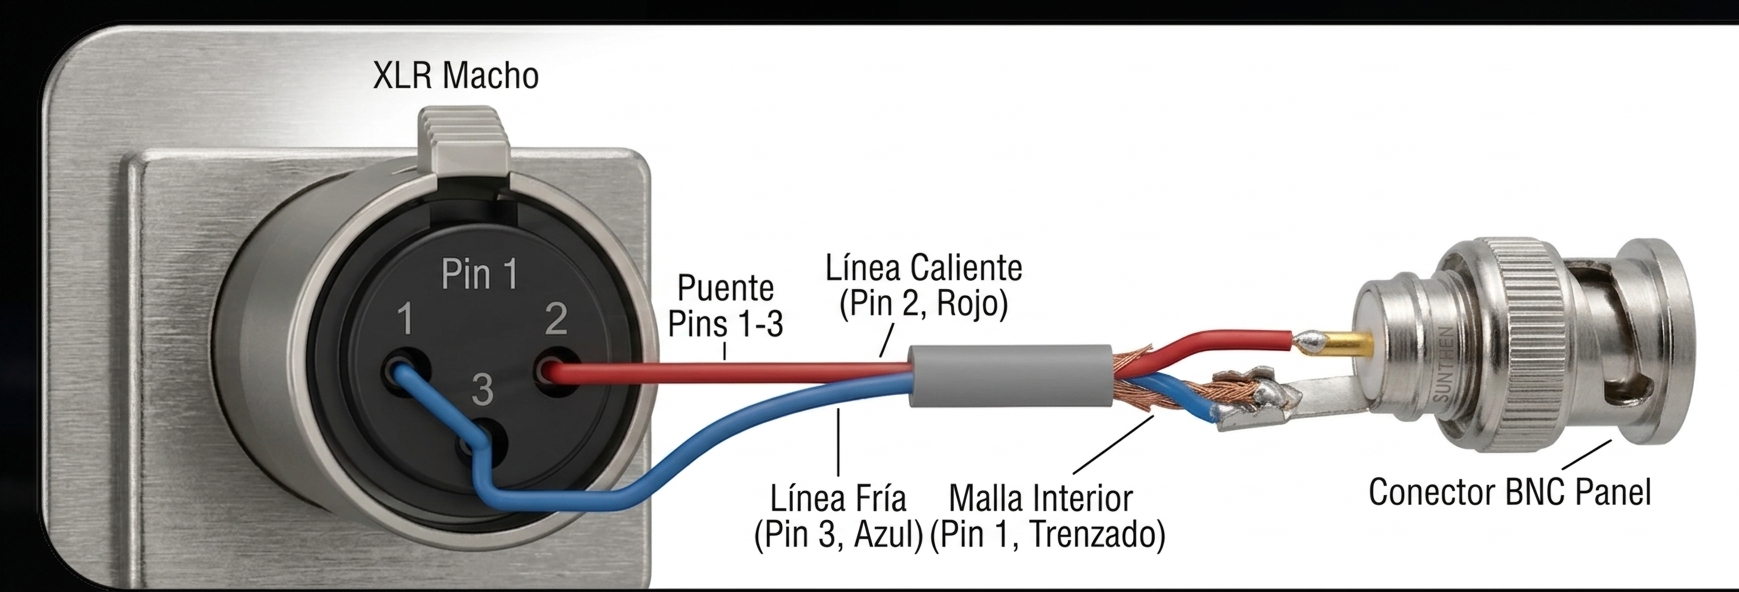
\includegraphics[width=0.7\textwidth,keepaspectratio]{figures/diagrama_xlr_bnc.png}
\caption[Adaptación XLR a BNC para entrada del NI-9234]{Esquema de adaptación de conector XLR macho a BNC para la entrada del módulo NI-9234. El pin~2 (línea caliente, rojo) y el pin~3 (línea fría, azul) configuran la señal balanceada, mientras que el pin~1 (malla, trenzado) se conecta a la malla interior del cable. Un puente entre los pines 1 y 3 adapta la señal balanceada al conector BNC asimétrico del módulo de adquisición.}
\label{fig:xlr-bnc}
\end{figure}


\subsection{Conexiones de instrumentos auxiliares (cámara y ESP32)}

Para la cámara microscópica y la alimentación/comunicación del nodo ESP32 se emplea un cable USB-A de extensión de 3 metros (Figura 26). Se elige un cable USB robusto y apantallado para minimizar pérdidas de señal y problemas de alimentación. Cuando la distancia o la caída de tensión son relevantes se favorece alimentar el ESP32 desde una fuente local estable y usar el USB únicamente para datos, o emplear un cable USB con alimentación reforzada (pared/estación). Además, se colocan filtros o aisladores si se detectan ruidos introducidos por la línea USB que afecten a la adquisición analógica principal.


\section{Desarrollo de software de adquisición de datos}

Para el desarrollo del sistema experimental se adopta \textbf{Python} como plataforma principal por su capacidad de integrar adquisición, preprocesado y análisis de señales en un único flujo reproducible, vistazo visual de Front-End en la Figura 27. Python facilita la conexión con instrumentación (p. ej. NI mediante nidaqmx), el tratamiento de audio (soundfile, librosa, scipy) y la construcción de una interfaz de operación confiable con PyQt (GUI,  Graphical User Interface). Esta combinación permite ejecutar workers de adquisición en segundo plano (multithreading), separar la lógica de captura de la de visualización y registrar metadatos de forma estructurada, requisitos imprescindibles para grabaciones largas y auditoría experimental.


La arquitectura software sintetiza tres responsabilidades: (i) adquisición y almacenamiento robusto (registro en streaming a TDMS y conversión controlada a WAV/índices en .db), (ii) control y orquestación a través de la GUI y main.py, y (iii) preprocesado y trazabilidad del pipeline (resampling, detección de clipping, extracción de features). Diseñar la pila con estos tres bloques asegura que cada ejecución sea reproducible, auditable y compatible con los análisis estadísticos y de aprendizaje automático presentados en el capítulo 7.

Las decisiones técnicas adoptadas (formato TDMS para escritura en disco, uso de un manifiesto con checksums y timestamps, y registro de versiones de código) responden a problemas prácticos detectados durante la puesta a punto ---memoria, estabilidad y sincronización multimodal--- y se describen y justifican en las subsecciones siguientes. Estas subsecciones desarrollan la integración NI, el subsistema ESP32, la estrategia de sincronización, el pipeline de conversión TDMS$\rightarrow$WAV$\rightarrow$DB y las rutinas de calibración y testing necesarias para garantizar la calidad de los datos experimentales.

\subsection{Resumen arquitectónico}

La Figura 28 muestra la arquitectura en cuatro capas: interfaz/orquestación, adquisición, registro/workers y análisis. La GUI actúa como panel de control y \texttt{main.py} coordina la ejecución delegando tareas a workers en segundo plano, lo que preserva la responsividad y la trazabilidad.

La adquisición integra tres subsistemas: el sistema de alta fidelidad (NI cDAQ-9174 + NI-9234), un nodo económico basado en ESP32 + micrófono INMP441 y una cámara microscópica CMOS para etiquetado visual. Esta combinación garantiza una “verdad de tierra” precisa y réplicas prácticas para validación en campo.

Se adopta TDMS (\textit{Technical Data Management Streaming}) como formato primario de registro por su escritura directa a disco y manejo eficiente de buffers (\textit{log \& read}), evitando acumulación de memoria y preservando estructura multicanal y timestamps precisos. TDMS exporta a WAV/CSV para análisis offline cuando hace falta.

Workers independientes realizan conversiones (TDMS $\rightarrow$ WAV/CSV), preprocesado (resampling, detección de clipping), extracción y agregación de features, y almacenamiento final. 


Esta separación minimiza uso de memoria en la GUI, facilita reinicios parciales y deja artefactos versionados para auditoría.

Todas las fuentes registran tiempos de registro (\textit{timestamps}) sincronizados y se genera un manifiesto por sesión con desplazamientos (\textit{offsets}) y calcula un valor hash (\textit{checksums}), lo que permite alinear audio, video y medidas auxiliares para etiquetado multimodal y análisis conjunto en el capítulo 7.

\subsection{Decisiones clave}

La arquitectura técnica del sistema nace de decisiones pragmáticas orientadas a garantizar \textbf{reproducibilidad}, \textbf{robustez} y \textbf{transferibilidad}. Se escoge Python como lenguaje principal por su ecosistema maduro para adquisición y análisis de señales (bibliotecas como nidaqmx, soundfile, librosa, scipy) y por la facilidad para integrar una interfaz gráfica (PyQt) que orquesta la instrumentación y registra metadatos de forma estructurada. Esta elección prioriza la portabilidad del software, la posibilidad de documentar y versionar el código (GitHub) y la capacidad de añadir pruebas automatizadas (testing) que respalden la validez experimental.

Para la adquisición de referencia se mantiene la plataforma de National Instruments: chasis NI cDAQ-9174 y módulo NI-9234. Esta combinación aporta muestreo multicanal a alta velocidad (51.2 kS/s por canal), resolución adecuada (24 bits) y filtros anti-aliasing integrados, requisitos que resultan imprescindibles para capturar transitorios y componentes de alta frecuencia de la emisión acústica en taladrado. Se usa este equipo como “verdad de tierra” (ground truth) cuya calidad y sincronización garantizan la validez de la base de datos para el modelado posterior.

El formato de almacenamiento primario se estandariza en TDMS (Technical Data Management Streaming). Después de evaluar CSV y bases de datos .db, TDMS resulta preferible porque permite escribir directamente a disco con baja latencia y soporta el patrón log-and-read, lo que evita la acumulación de memoria observada con escrituras en buffers y trazado en tiempo real. Esta decisión resuelve el problema operativo de “rampa” de memoria (memory leak/buildup) y mantiene el consumo de RAM estable, además de preservar la estructura multicanal y los timestamps precisos necesarios para el procesamiento posterior (conversión controlada a WAV para análisis offline).

Como estrategia híbrida se incorpora un subsistema de bajo coste basado en ESP32 con micrófono digital INMP441 y un caudalímetro YF-S201. Esta decisión multiplica la variedad sensórica y permite comparar performance entre un sistema de laboratorio (NI) y soluciones económicas replicables en entornos industriales pequeños (PYMEs). Esa heterogeneidad sensorial facilita estudios de adaptación de dominio (domain adaptation) y ayuda a construir modelos más generalizables, sin depender exclusivamente de instrumentación de referencia.

La captura visual se integra mediante una cámara microscópica CMOS sincronizada con las paradas programadas de la rutina de taladrado. La decisión de incluir imágenes de flanco como etiqueta visual responde a la necesidad de vincular métricas acústicas con evidencia física del desgaste (criterio VB), apoyando la creación de etiquetas fiables y multimodales para entrenamiento y validación.

En lo relativo a software de control y operación, la interfaz (PyQt) emplea un patrón de ejecución basado en \textit{workers}\footnote{Un \textit{worker} es un objeto de trabajo en segundo plano que ejecuta una tarea larga (adquisición, escritura a disco, conversión de formato) sin bloquear el hilo principal responsable de la interfaz gráfica \cite{moore2019}.} e hilos (\textit{multithreading}) para separar la adquisición, el almacenamiento y la visualización \cite{moore2019}. Esta separación mitiga bloqueos y permite que la escritura a TDMS se ejecute sin interferir con la GUI. Se define además un manifiesto de ejecución (manifest) y un mecanismo de logging detallado que registran versiones de software, parámetros de adquisición y checksums ---prácticas que aseguran trazabilidad y facilitan auditorías experimentales.

Finalmente, cada decisión incorpora un balance entre calidad y escalabilidad donde NI aporta fidelidad y sincronía, TDMS garantiza rendimiento y trazabilidad, ESP32 aporta economía y diversidad sensórica, y la GUI con workers garantiza operación controlada.

\subsection{Integración NI (cDAQ-9174 + NI-9234)}

La integración con National Instruments se diseña para asegurar una verdad de tierra (ground truth) de alta fidelidad y trazabilidad. El sistema captura audio multicanal a 51.2 kS/s por canal con resolución de 24 bits y filtro anti-aliasing integrado (NI-9234), lo que permite registrar transitorios rápidos y contenido espectral relevante para detección de desgaste.

La configuración y control del módulo se realiza desde la capa Python mediante el driver oficial (nidaqmx / NI API). Se registran y versionan los perfiles de canal (mapa de canales y su descripción), ganancias (gains), rango de entrada, tipo de acondicionamiento (preamplificador, IEPE si aplica), sample rate y la fuente de reloj (sample clock). La adquisición utiliza un clock de muestreo y triggers hardware definidos para garantizar que las marcas temporales (timestamps) sean precisas y sincronizables con la cámara y con los nodos ESP32.

Como práctica operativa se documenta un manifiesto por sesión que incluye: nombre de archivo TDMS, mapeo de canales, offsets temporales, parámetros de adquisición y checksums (hash) para cada fichero. Para la escritura se emplea TDMS en modo log-and-read ---escritura directa a disco por bloques--- evitando mantener grandes buffers en memoria y mitigando la acumulación de RAM durante grabaciones prolongadas. A efectos de visualización en la GUI, se leen porciones (chunks) del TDMS para representación en tiempo real sin interferir con la grabación continua.

\subsection{Subsistema MCU (ESP32 + INMP441 + caudalímetro)}

El nodo ESP32 funciona como un registrador económico que captura dos tipos de información: audio (con un micrófono digital tipo INMP441) y el caudal de refrigerante (sensor YF-S201). Durante la ejecución guarda ambas señales en una tarjeta micro-SD: un archivo de audio en formato WAV provisional y un fichero CSV con lecturas del caudal cada segundo. El dispositivo gestiona la captura en segundo plano para que la escritura a tarjeta y la lectura del sensor no interfieran entre sí, y asegura que los datos se guarden periódicamente para evitar pérdidas.

La interacción con el ESP32 se realiza por una pequeña API HTTP donde comandos simples permiten iniciar la grabación (/start), detenerla (/stop) y descargar los ficheros desde la GUI (/download, /download\_flow). Al detener la grabación, el equipo actualiza correctamente el encabezado del WAV (para que el archivo sea reproducible) y envía ambos archivos al servidor de almacenamiento del laboratorio mediante una petición HTTP. Para mantener los tiempos coherentes entre equipos, el ESP32 sincroniza su reloj con servidores de tiempo en la red (NTP), así los registros llevan marcas temporales comparables con las del resto de sensores.

Se incorporan medidas prácticas de robustez que aseguran la continuidad de la adquisición. Antes de iniciar cada ensayo se verifica el estado de la tarjeta micro-SD y se crea un espacio de almacenamiento exclusivo para la sesión. Durante la grabación, los datos se guardan de forma periódica en disco para minimizar pérdidas en caso de interrupción. Esta estrategia resulta necesaria porque la memoria \textit{flush} interna de la ESP32 no permite sostener grabaciones de audio largas y de buena calidad con el micrófono digital; por ello, la información se conserva en crudo directamente en la micro-SD, lo que habilita registros extensos y reduce el riesgo de sobrescrituras accidentales.

La calidad de muestreo representa una limitación conocida, es la propia de un nodo económico (ej. 16 kHz), por lo que se considera como complemento a los registros de alta fidelidad del equipo NI, no como sustituto completo. También, el envío por HTTP requiere que el receptor (el ordenador de almacenamiento) esté accesible en la misma red local; si la red institucional impone restricciones, puede fallar la transferencia automática.

\textbf{Consideraciones de conectividad institucional.} Dado que la red corporativa de la universidad exige autenticación y no permite que el ESP32 y el computador de almacenamiento compartan subred directamente, se empleó un punto de acceso WiFi portátil como solución de red local para la transferencia de archivos entre ambos dispositivos.

\clearpage
\chapter{Ensayos realizados}

La campaña experimental del presente trabajo se organizó en dos bloques complementarios. Un primer bloque de \textbf{ensayos hasta el estado de falla} tuvo como objetivo reproducir ---en las instalaciones de la UIS y con el equipamiento propio de esta tesis--- la progresión completa de desgaste documentada por \citeA{orejarena2014}, llevando cada broca desde el estado nuevo hasta la fractura del filo. Un segundo bloque de \textbf{ensayos sin inducción de falla} se concibió como banco de pruebas del sistema multimodal completo (NI + ESP32 + caudalímetro + cámara microscópica): se instrumentaron tandas de agujeros sucesivos con la misma broca, registrando audio, caudal de taladrina y evidencia visual del flanco entre ciclos, pero deteniendo la corrida antes de alcanzar la fractura. En ambos bloques el material base fue acero SAE~4140 en forma de discos cilíndricos previamente mecanizados (Figura~\ref{fig:discos-material}), sujetos en la copa universal descrita en el Capítulo~3 y taladrados en el centro de mecanizado Leadwell V-20 del laboratorio (Figura~\ref{fig:leadwell-cap5}) siguiendo los parámetros de corte calculados para las brocas Dormer A100 de 6 y 8\,mm.

\begin{figure}[htbp]
\centering
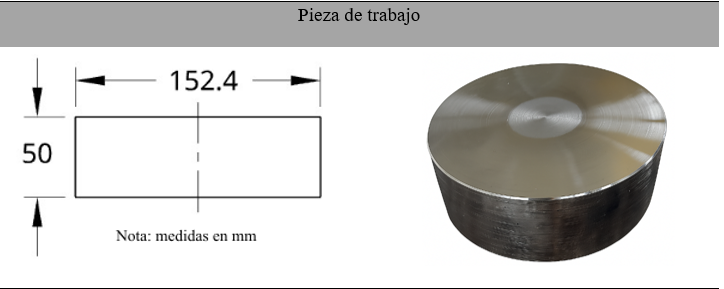
\includegraphics[width=0.55\textwidth,keepaspectratio]{figures/img_006.jpg}
\caption[Discos de acero SAE 4140 para los ensayos]{Discos cilíndricos de acero SAE~4140 preparados como material de ensayo. La cara superior muestra el refrentado previo al taladrado y el lateral revela la capa de cascarilla de laminación que fue eliminada antes de montarlos en la copa de sujeción.}
\label{fig:discos-material}
\end{figure}

\begin{figure}[htbp]
\centering
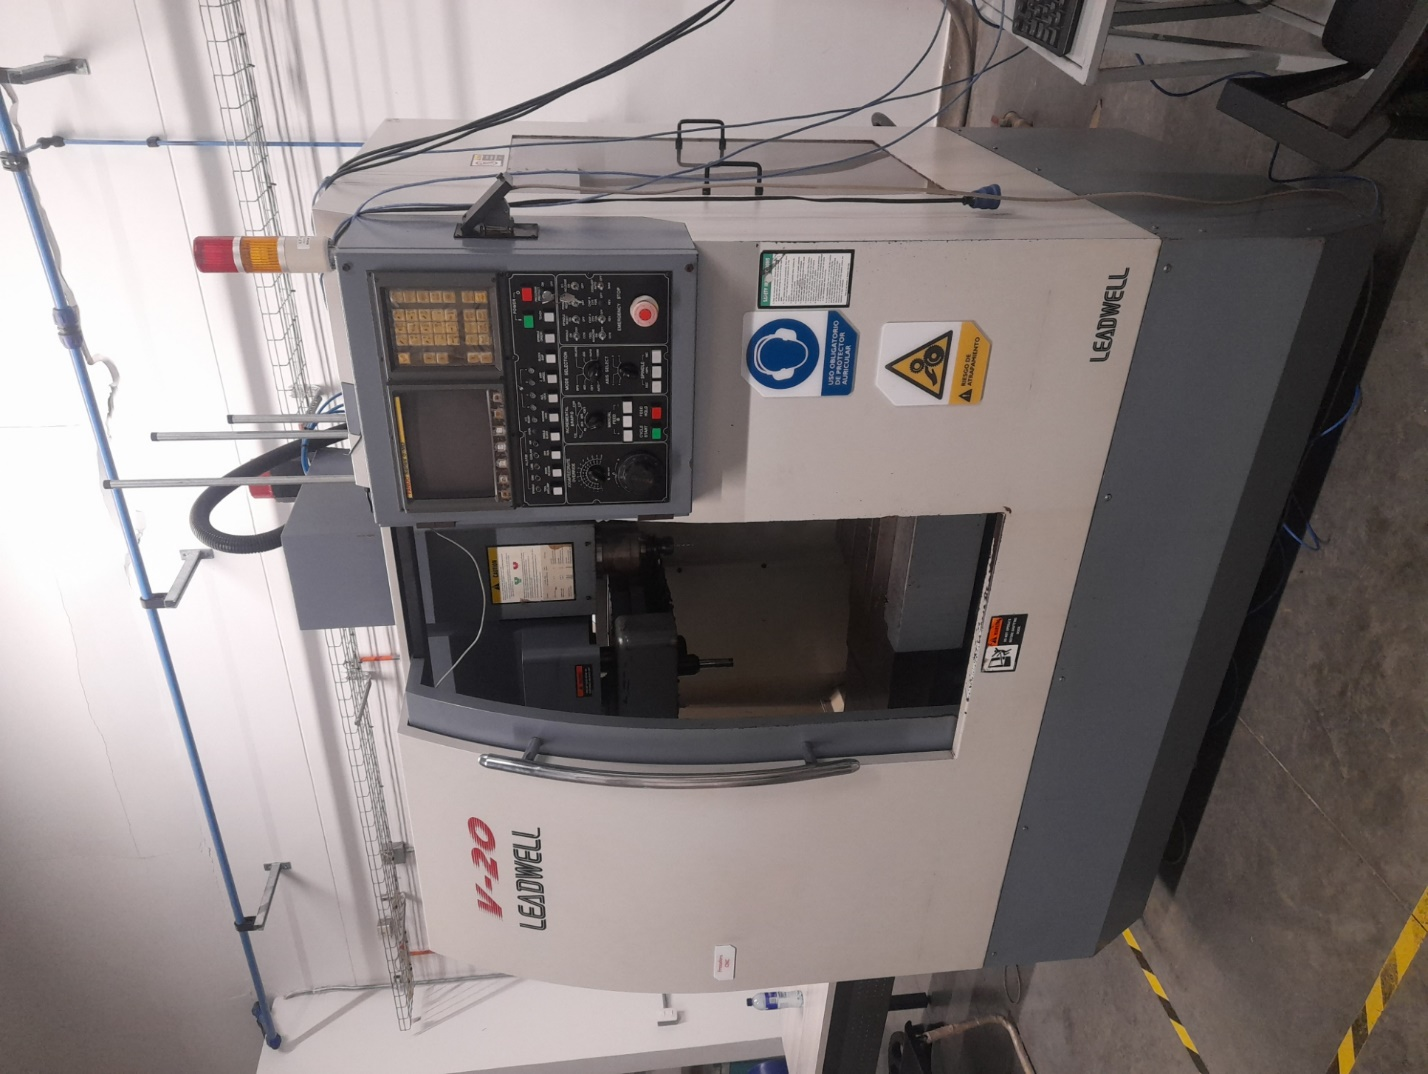
\includegraphics[width=0.55\textwidth,keepaspectratio]{figures/img_008.jpg}
\caption[Centro de mecanizado Leadwell V-20 empleado en los ensayos]{Centro de mecanizado vertical Leadwell V-20 (control Fanuc) del Laboratorio de Manufactura de la UIS, plataforma común a todos los ensayos de este trabajo.}
\label{fig:leadwell-cap5}
\end{figure}

Siguiendo la numeración análoga al Lote~I (\citeA{orejarena2014}, experimentos E1--E7), los ensayos propios del presente trabajo se designan como \textbf{E8} en adelante, agrupados por la broca empleada en cada cadena. La Tabla~\ref{tab:ensayos-lote2} resume la configuración y el total de registros por ensayo, y el detalle narrativo se desarrolla en las dos secciones siguientes.

\begin{table}[htbp]
\centering
\caption{Resumen de ensayos del Lote~II: configuración, duración (agujeros perforados) y volumen de datos recogido por modalidad. Los audios NI agregan los tres canales sincronizados (MAXLIN UDM-51, Behringer SL84C, Behringer C1); los registros ESP32 corresponden al par audio INMP441 + CSV de caudal YF-S201.}
\label{tab:ensayos-lote2}
\small
\begin{tabular}{@{}llccccc@{}}
\toprule
Ensayo & Broca & $\varnothing$ (mm) & Agujeros & Audios NI & Imágenes $\mu$-scopio & Registros ESP32 \\
\midrule
\multicolumn{7}{@{}l@{}}{\textit{Ensayos hasta el estado de falla}} \\
E8  & Dormer A100 \#1 & 6 & 140 & 420 & 28 & --- \\
E9  & Dormer A100 \#2 & 6 &  37 & 111 &  8 & --- \\
E10 & Dormer A100 \#3 & 6 &  55 & 165 & 11 & --- \\
\midrule
\multicolumn{7}{@{}l@{}}{\textit{Ensayos sin inducción de falla}} \\
E11 & Dormer A100 \#4 & 6 & 110 & 330 & 22 & 1 \\
E12 & Dormer A100 \#5 & 6 &  95 & 285 & 19 & 1 \\
E13 & Dormer A100 \#6 & 6 &  90 & 270 & 18 & 1 \\
E14 & Dormer A100 \#7 & 8 &  48 & 144 & 10 & 1 \\
\midrule
\textbf{Total} & \textbf{7 brocas} & --- & \textbf{575} & \textbf{1\,725} & \textbf{116} & \textbf{4} \\
\bottomrule
\end{tabular}
\end{table}

\section{Ensayos hasta el estado de falla}

Este bloque agrupa los ensayos E8, E9 y E10, ejecutados sobre el disco-copa del Capítulo~3 con la configuración de tres micrófonos ya descrita y adquisición de referencia vía NI cDAQ-9174 + NI-9234 a 51{,}2\,kS/s por canal. Cada ensayo consistió en perforar agujeros ciegos consecutivos con la misma broca siguiendo una rutina G81 sobre la red de posiciones fresadas en la copa, hasta provocar la fractura del filo. Entre agujeros se mantuvo la broca montada en el husillo, lo que permitió observar la deriva de los descriptores acústicos dentro de una misma sesión sin introducir variabilidad por montaje. La cámara microscópica se activó de forma programada en las paradas previstas por la rutina, registrando la evolución del flanco y el criterio VB en intervalos homogéneos de agujeros \cite{groover2007}.

\begin{figure}[htbp]
\centering
\begin{minipage}{0.48\textwidth}\centering

\includegraphics[width=\textwidth,keepaspectratio]{{figures/material taladrado en sujecion de copa}.jpeg}\\
\small (a) Taladrado en curso sobre la copa.
\end{minipage}\hfill
\begin{minipage}{0.48\textwidth}\centering
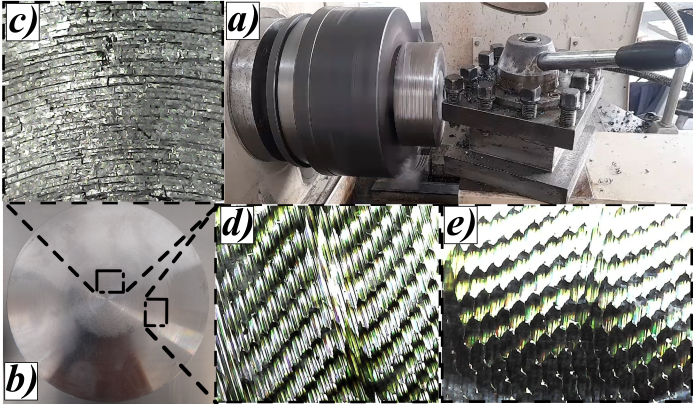
\includegraphics[width=\textwidth,keepaspectratio]{figures/img_015.png}\\
\small (b) Evidencia del desgaste y fractura del flanco.
\end{minipage}
\caption[Ensayo representativo del bloque hasta falla]{Ensayo representativo del bloque hasta falla. (a)~Taladrado en curso de un agujero ciego sobre uno de los discos alojados en la copa de sujeción; la viruta visible en primer plano corresponde al último agujero perforado. (b)~Evolución del flanco registrada por la cámara microscópica: montaje inicial, desgaste intermedio, filo desgastado antes del fallo y superficie del filo tras la fractura con el cráter de ruptura frágil.}
\label{fig:taladrado-falla-desgaste}
\end{figure}

La cadena principal (ensayo~E8) totalizó 140 agujeros antes de la fractura con la primera broca Dormer A100 de 6\,mm. Una vez sustituida la herramienta se ejecutaron dos cadenas más cortas: E9 con 37 agujeros y E10 con 55 agujeros, variando ligeramente los parámetros de avance para cubrir trayectorias de desgaste de distinta duración. Las tres brocas terminaron con fractura del filo en el último agujero, verificada tanto por el salto característico en la señal acústica como por la inspección visual posterior (Figura~\ref{fig:taladrado-falla-desgaste}b).

En paralelo a la adquisición acústica se registró el progreso de cada ensayo en la base de conocimiento de la GUI (Figura~\ref{fig:gui-base-conocimiento}), construida bajo un patrón de arquitectura por vistas y \textit{workers} independientes \cite{moore2019}: la interfaz mantiene tres paneles ---uno por micrófono--- y una barra de progreso que indica el porcentaje de vida útil consumida por la broca activa, calculado a partir del número de agujeros previsto por los parámetros de corte y la fractura observada. Esta vista permite al operario detectar desviaciones tempranas respecto al comportamiento esperado y descartar ensayos afectados por incidencias (p.~ej. pérdida de un canal, saturación o interrupción del caudal de taladrina).

\begin{figure}[htbp]
\centering
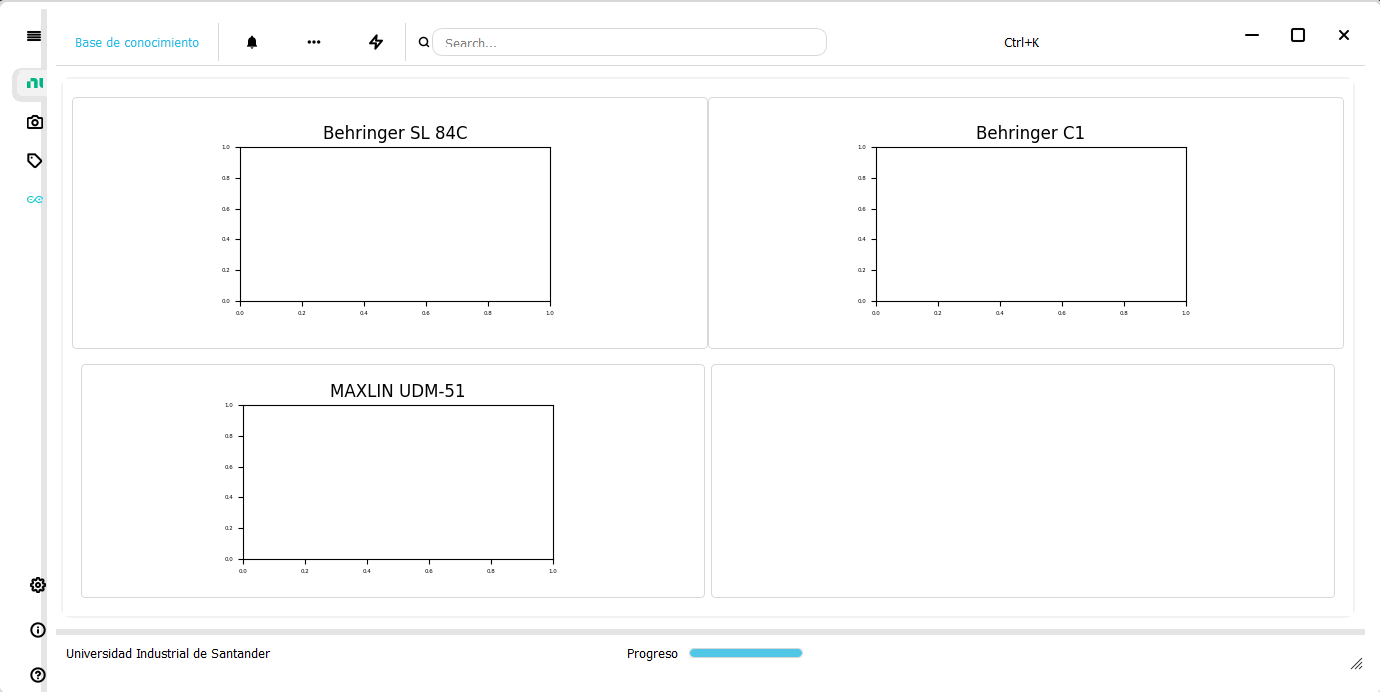
\includegraphics[width=0.95\textwidth,keepaspectratio]{figures/img_045.png}
\caption[Panel de base de conocimiento de la GUI durante un ensayo]{Panel ``Base de conocimiento'' de la GUI mostrando los tres canales activos (Behringer SL84C, Behringer C1 y MAXLIN UDM-51) y el progreso de la broca en curso (barra inferior). Cada subventana agrupa los agujeros ya procesados por canal y permite al operario comparar en tiempo real la respuesta de los tres micrófonos frente al mismo evento de corte.}
\label{fig:gui-base-conocimiento}
\end{figure}

La Figura~\ref{fig:montaje-real-micros} documenta el montaje definitivo del arreglo de micr\'{o}fonos sobre la m\'{a}quina tal como se ejecut\'{o} durante los ensayos de este bloque, donde se aprecian las tres unidades alineadas respecto al husillo, los drip-loops y la ruta de cable hacia el rack del NI-9234; este registro se incluy\'{o} en el manifiesto de cada sesi\'{o}n para fines de trazabilidad y control de calidad.

\begin{figure}[htbp]
\centering
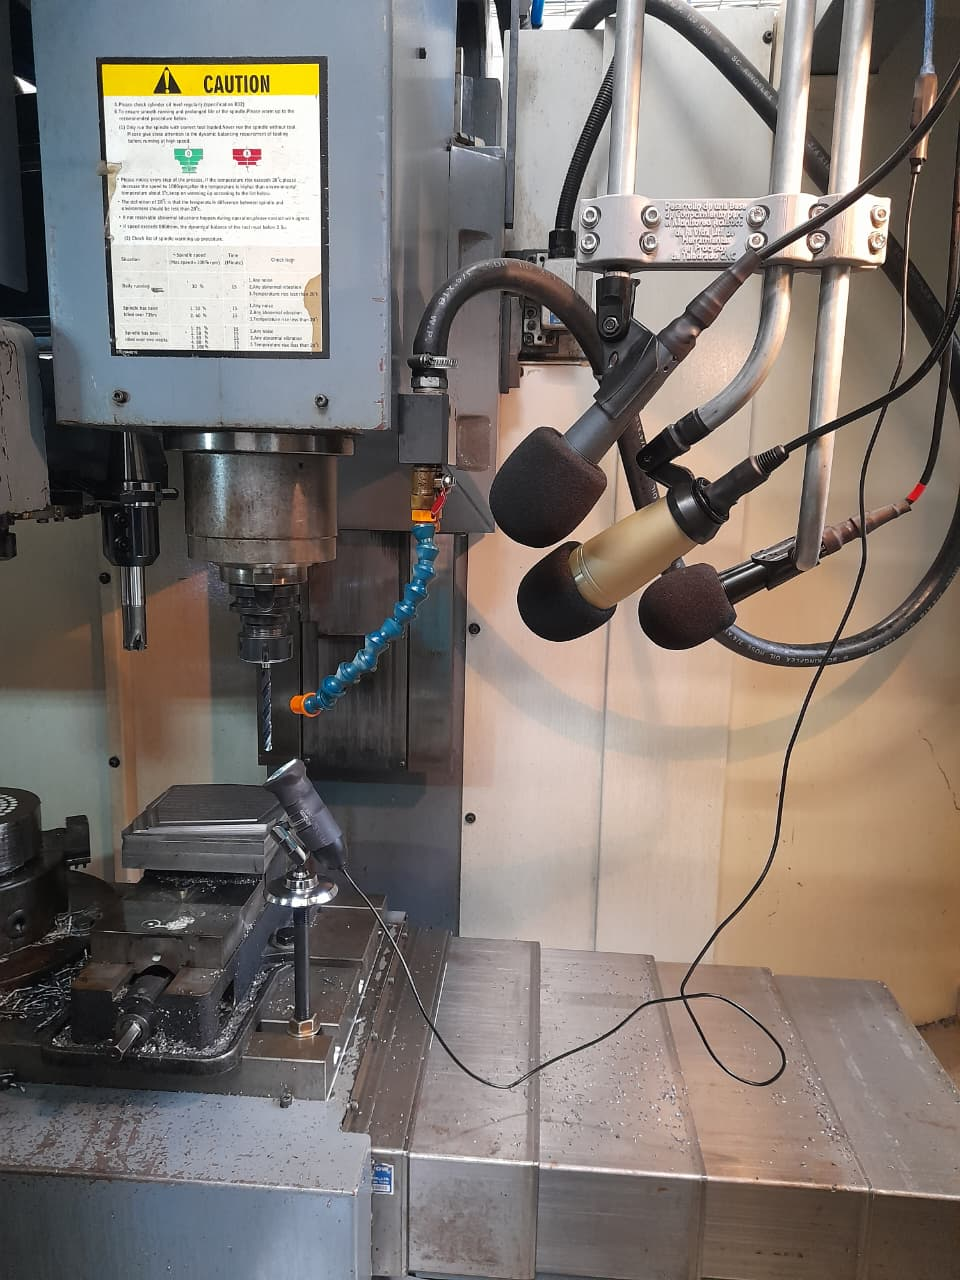
\includegraphics[width=0.82\textwidth,keepaspectratio]{figures/montaje_real_microfonos_maquina.jpeg}
\caption[Montaje real de los micr\'{o}fonos sobre la m\'{a}quina]{Montaje real del arreglo de micr\'{o}fonos sobre la pared acr\'{i}lica del Leadwell V-20 durante los ensayos del bloque hasta falla. Se observan las tres unidades equidistantes respecto al husillo, las abrazaderas con termo-retr\'{a}ctil y la ruta de cableado balanceado hacia el rack del NI-9234, fotografiada en cada sesi\'{o}n como control de calidad del montaje.}
\label{fig:montaje-real-micros}
\end{figure}

El producto final de este bloque fueron 232 agujeros segmentados, con triple registro acústico (tres muestras por agujero, una por micrófono) y etiquetado ordinal de desgaste derivado del cociente \texttt{hole\_number / total\_holes} con los cortes [15\,/\,75]\,\% establecidos en el Capítulo~3. La Figura~\ref{fig:grafico-brocas-desgaste} sintetiza la progresi\'{o}n de agujeros perforados por cada una de las siete brocas empleadas en el Lote~II, permitiendo visualizar las distintas trayectorias de vida \'{u}til y el punto de fractura alcanzado en los ensayos del bloque hasta falla frente al corte controlado de los ensayos sin inducci\'{o}n de falla. Este subconjunto constituye la columna vertebral del \textit{dataset} extendido sobre el que se construyen los resultados de los capítulos siguientes.

\begin{figure}[htbp]
\centering
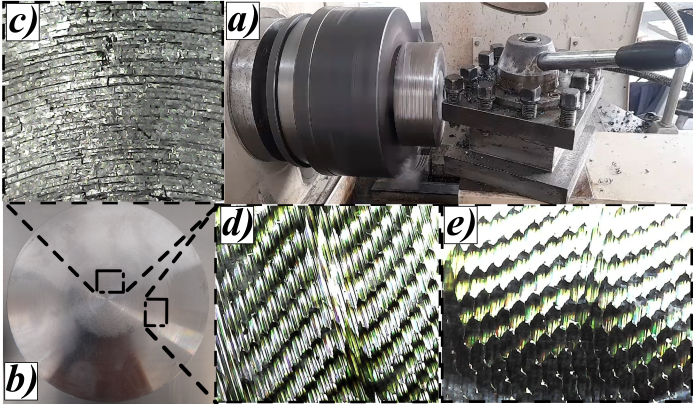
\includegraphics[width=0.85\textwidth,keepaspectratio]{figures/grafico_brocas_desgaste.png}
\caption[Progresi\'{o}n de agujeros por broca en el Lote~II]{Progresi\'{o}n de agujeros perforados por cada una de las siete brocas Dormer A100 empleadas en los ensayos E8--E14. Las barras resaltan las tres brocas llevadas hasta el estado de falla (E8--E10) y las cuatro brocas detenidas antes de la fractura (E11--E14) utilizadas como banco de pruebas del \textit{pipeline} multimodal.}
\label{fig:grafico-brocas-desgaste}
\end{figure}

\section{Ensayos sin inducción de falla}

El segundo bloque (ensayos E11--E14) se concibió como banco de pruebas del \textit{pipeline} multimodal completo, incluyendo el nodo ESP32 con micrófono INMP441 y caudalímetro YF-S201 presentado en el Capítulo~4. A diferencia del bloque anterior, aquí se fijó un número máximo de agujeros por ensayo y se detuvo la corrida antes de alcanzar la fractura, preservando así la broca para inspección microscópica. Esta estrategia permitió obtener trayectorias de desgaste \emph{tempranas} (hasta \textasciitilde50\,\% de la vida útil prevista), complementarias a las trayectorias \emph{completas} del bloque anterior, y verificar la correcta integración del sensor de caudal en la cadena de adquisición.

\begin{figure}[htbp]
\centering
\begin{minipage}{0.42\textwidth}\centering
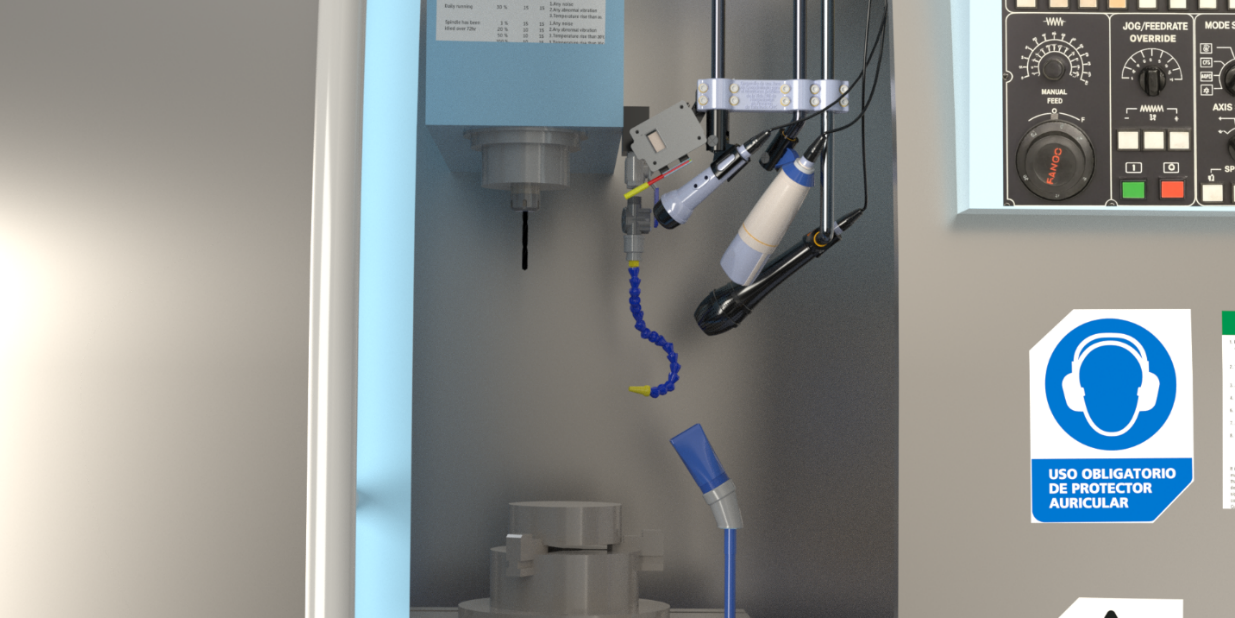
\includegraphics[width=\textwidth,keepaspectratio]{figures/img_037.png}\\
\small (a) Micrófono de pértiga sobre la zona de corte.
\end{minipage}\hfill
\begin{minipage}{0.52\textwidth}\centering
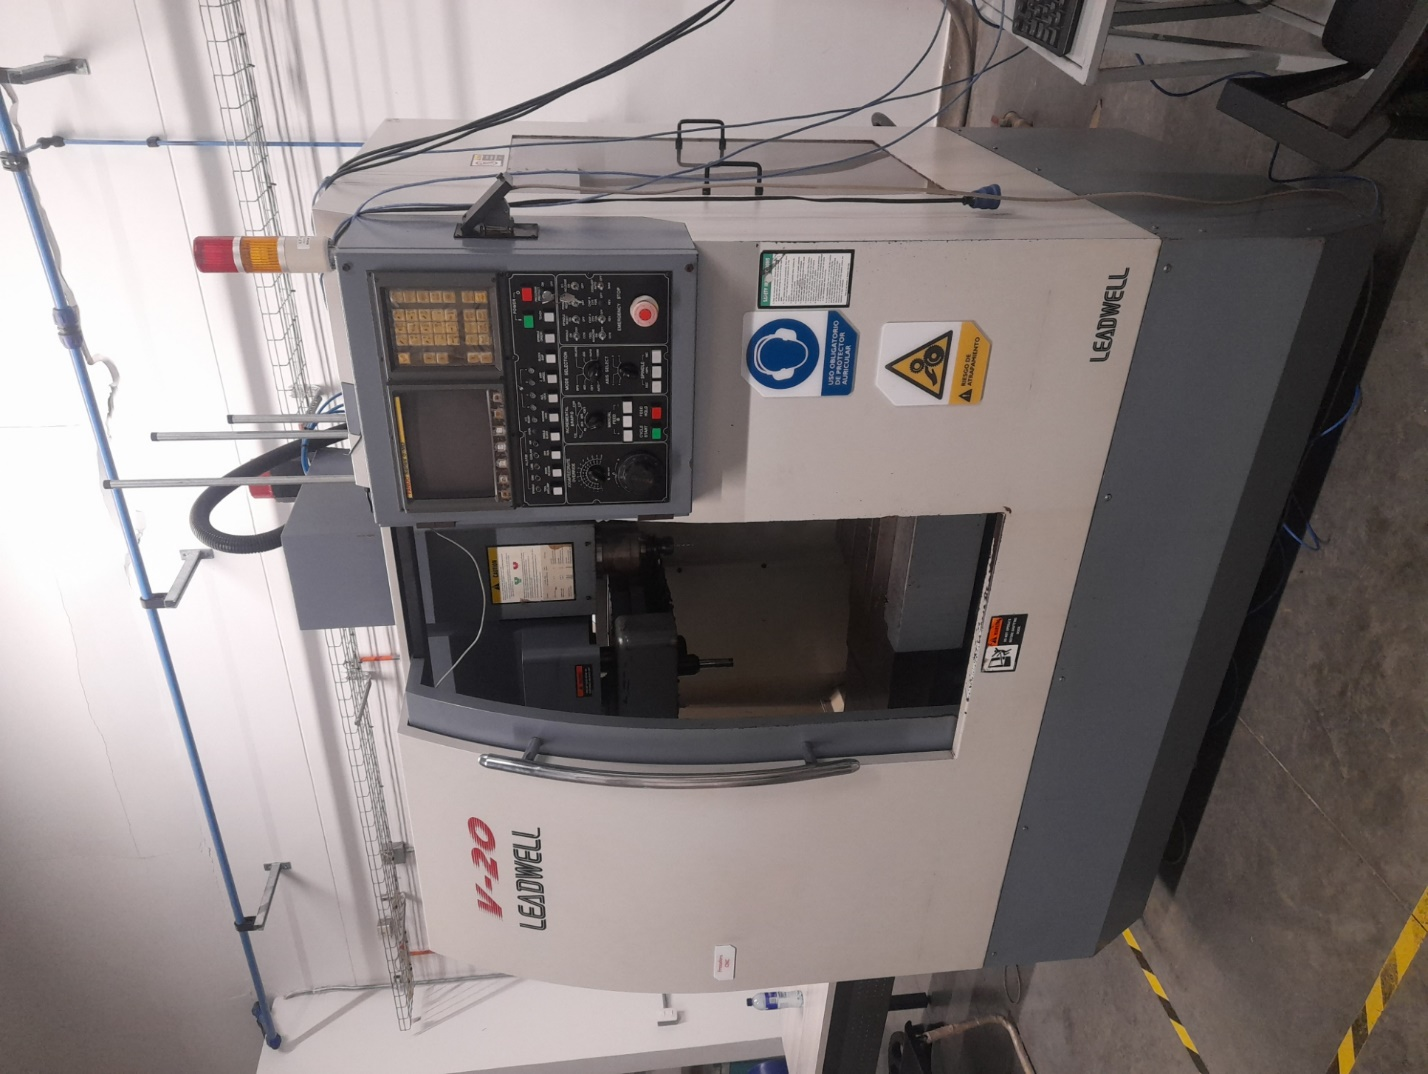
\includegraphics[width=\textwidth,keepaspectratio]{figures/laboratorio_leadwell_real.jpg}\\
\small (b) Laboratorio de manufactura con la Leadwell V-20.
\end{minipage}
\caption[Montaje del bloque sin inducción de falla]{Montaje del bloque sin inducción de falla. (a)~Micrófono de pértiga suspendido sobre la zona de corte y conectado por cable balanceado al rack del NI-9234 situado fuera de la cabina; la señalización lateral recuerda el uso obligatorio de protección auditiva durante los ciclos de taladrado. (b)~Vista general del laboratorio de manufactura: banco instrumental, Leadwell V-20 al fondo y estación de ESP32 con tarjeta microSD preparada para iniciar una sesión de adquisición.}
\label{fig:montaje-sin-falla}
\end{figure}

El ensayo representativo de este bloque (E11) empleó la cuarta broca Dormer A100 de 6\,mm durante 110 agujeros. El registro multimodal incluyó: (i)~tres canales NI a 51{,}2\,kS/s, (ii)~audio INMP441 a 16\,kHz muestreado desde el ESP32, (iii)~CSV de caudal \texttt{flow.csv} con una lectura por segundo del YF-S201 y (iv)~capturas periódicas del flanco mediante la cámara microscópica. La sincronización entre fuentes se verificó \emph{a posteriori} contrastando los picos de actividad acústica con las bajadas del caudal asociadas a la activación de la electroválvula de taladrina, siguiendo el procedimiento descrito en el Capítulo~4. Los ensayos E12--E14 replicaron el mismo protocolo variando el diámetro de broca y el número total de agujeros para cubrir un rango más amplio de trayectorias.

Los aprendizajes operativos de este bloque ---principalmente la necesidad de un punto de acceso WiFi dedicado para el ESP32 y de marcar los agujeros por software en lugar de hacerlo mediante anotaciones manuales--- se consolidaron en la versión final del protocolo experimental. Los datos agregados de E11--E14 (343 agujeros) conforman, junto con los ensayos hasta la falla del bloque anterior, el subconjunto del Lote~II sobre el que se construyen los resultados comparativos de los capítulos posteriores.

\clearpage
\chapter{Procesamiento de las señales}

\section{Descripción del dataset de Orejarena}

El \textit{dataset} utilizado en esta parte del trabajo proviene del estudio de \citeA{orejarena2014}. Los registros experimentales originales están almacenados en formatos propios del entorno de adquisición: principalmente archivos \texttt{.lvm} (formato tabulado de National Instruments/LabVIEW) y archivos MATLAB (\texttt{.mat}). En total el conjunto contiene aproximadamente 2010 grabaciones correspondientes a cada operación de taladrado con ciclo G81, junto con metadatos experimentales asociados (p.~ej. identificador de ensayo, tipo de broca, micrófono empleado y registro temporal). A partir de la documentación y las señales disponibles se infirieron inicialmente dos etiquetas (\emph{sin desgaste} y \emph{con desgaste}) más una categoría de ruidos de fondo; durante este proyecto dicho etiquetado binario se reestructuró a una escala ordinal de tres estados: \textbf{Estado~0} (sin desgaste), \textbf{Estado~1} (medianamente desgastado) y \textbf{Estado~2} (desgastado), acorde con la región de etiquetado establecida al 15\,\% y 75\,\% del ciclo de vida útil de cada broca. La estructura general del primer grupo de ensayos se organiza por experimentos ``E\textit{x}'' (donde \textit{x} es el identificador), agrupados a su vez por tipo de broca y micrófono empleados.

\section{Pipeline de procesamiento y extracción de características}

A continuación se detalla de forma compacta el flujo de procesamiento implementado en los \textit{scripts} principales \texttt{feature\_analysis\_drilling\_v5.py} y \texttt{analyze\_v5\_fixed.py}.\footnote{\textit{Repositorio:} \href{https://github.com/OscarAyalaO/pipeline_SVM}{\texttt{github.com/OscarAyalaO/pipeline\_SVM}} (scripts de extracción de descriptores y análisis exploratorio).} El objetivo de esta sección es mostrar ---sin entrar en exceso técnico--- qué hace el \textit{pipeline}, por qué se hacen esas operaciones y qué archivos produce, de modo que el lector de la tesis pueda reproducir y entender la cadena lógica del análisis.

El \textit{pipeline} toma como entrada una \textbf{carpeta raíz} que contiene los audios ya convertidos a WAV (PCM sin compresión) organizados por carpetas temáticas ---sin desgaste, con desgaste y ruidos--- y procesa cada archivo de forma independiente para extraer un conjunto amplio de características acústicas. Estas características se agregan por archivo (media y desviación estándar de las medidas por \textit{frame}, indicadores de valores atípicos, etc.) y se exportan a CSV para su análisis estadístico y modelado posterior.

Dado que los ficheros originales estaban en .lvm y .mat, y que la mayoría de las herramientas de procesamiento de audio empleadas en este proyecto trabajan de forma nativa con formas de onda estándar, se llevó a cabo una conversión controlada de los .lvm a archivos de audio en formato WAV (PCM sin compresión). El flujo de conversión está documentado en el cuadernillo \textit{Conversion total REAL.ipynb}  y consistió en los pasos siguientes:

\textbf{Verificación y normalización}: comprobación de consistencia en la tasa de muestreo y normalización de amplitud cuando fue necesario para garantizar homogeneidad entre clips.

\textbf{Exportación a WAV}: escritura de señales en archivos .wav en formato PCM lineal de 16 bits, preservando la resolución temporal y la dinámica de la señal original.

\textbf{Registro y trazabilidad}: para cada archivo convertido se guardó un registro que vincula el .lvm original, el .mat (cuando aplica) y el .wav resultante, junto con las etiquetas inferidas y metadatos experimentales.

 La decisión de convertir y trabajar con WAV se fundamenta en criterios de integridad y reproducibilidad del análisis acústico: los WAV en PCM preservan picos, transitorios y la distribución espectral completa sin introducir artefactos por compresión con pérdida, elementos que son críticos para la extracción de características (p.~ej. \textit{spectral rolloff}, MFCC, medidas de energía y métricas basadas en transitorios). Esto reduce el riesgo de alterar índices acústicos sensibles y facilita la comparación con la literatura que advierte sobre los efectos negativos de la compresión en tareas de detección y clasificación sonora. Por tanto, todos los audios empleados en los análisis presentados en los apartados siguientes se almacenan y procesan en formato WAV (PCM sin compresión) para garantizar la validez de las métricas computadas y la trazabilidad del procesamiento.

\subsection{Origen de las características acústicas extraídas}

Se seleccionaron descriptores representativos de tres dominios físicos: \textbf{timbre} (\textit{centroid}, MFCC, \textit{flatness}, \textit{chroma}), \textbf{energía} (RMS, \textit{peak}, energía Mel/\textit{wavelet}, factor de cresta) y \textbf{temporal/rítmico} (duración, tasa de \textit{onsets}, \textit{tempo}). Estas medidas se calculan por tramo (\textit{frames} de entre 20 y 50~ms) y se agregan por archivo mediante estadísticos resumen (media y desviación estándar) para producir \texttt{features\_per\_file.csv}. La lista completa de variables y sus definiciones físicas se presenta en el Apéndice~\ref{ap:descriptores-acusticos}.

\subsection{Algoritmo de extracción de características basado en base de datos inicial}

\noindent La extracción de características parte de la colección de WAV ya convertidos y organizados por carpetas temáticas. Por cada archivo el extractor computa un conjunto homogéneo de medidas temporales, espectrales y multiescala (RMS, pico, centroide, \textit{rolloff}, MFCC, energía por escalas CWT, planitud, tonalidad, métricas de transitorios, etc.). Estas medidas, inicialmente calculadas por tramo o \textit{frame}, se agregan por archivo ---mediante media y desviación estándar--- y se registran en un archivo maestro \texttt{features\_per\_file.csv}. Cuando existen múltiples versiones de extracción (v2, v3), un procedimiento de fusión automático construye \texttt{merged\_features\_raw.csv}, evitando duplicados y preservando la trazabilidad mediante campos como \texttt{filepath}, \texttt{source}, \texttt{experiment} y \texttt{mic}.

\noindent El diseño prioriza la reproducibilidad al conservar metadatos de cada WAV, lo que permite vincularlo con su origen (\texttt{.lvm}/\texttt{.mat}), y el proceso registra el mapeo entre formatos y la firma \textit{checksum} de los archivos convertidos. De este modo, la tabla final contiene por fila un identificador único por audio y todos los atributos necesarios para el análisis posterior.

\subsection{Análisis exploratorio y criterios de selección}

Sobre la tabla consolidada se aplica un proceso de limpieza (coerción numérica, eliminación de columnas con alto porcentaje de NaN, resumen de columnas tipo \textit{array-like}) y detección de valores atípicos mediante \textit{Tukey fences} y percentiles extremos. La evaluación estadística combina ANOVA factorial (cuando se cumplen los supuestos) con pruebas no paramétricas (Kruskal--Wallis) y medidas de tamaño del efecto ($\eta^2$, \textit{d} de Cohen). Para modelado supervisado se emplea imputación por la mediana con estandarización posterior y validación agrupada (\textit{GroupKFold}\footnote{Método de validación cruzada que garantiza que muestras provenientes del mismo ensayo o broca no aparezcan simultáneamente en los conjuntos de entrenamiento y prueba, evitando sobreestimar el rendimiento del clasificador.}) para prevenir fugas de información; la interpretabilidad se apoya en \textit{permutation importance} y SHAP.

\subsubsection{Análisis de Varianza (ANOVA)}

El ANOVA es una prueba estadística clásica para comparar las medias de tres o más grupos, con el objetivo de determinar si al menos una de esas medias difiere significativamente del resto. \citeA{montgomery2013} definen el ANOVA como una herramienta para diseñar experimentos en ingeniería donde se disecciona la variabilidad total de la respuesta en componentes atribuibles a distintos factores (entre-grupos) frente a la variabilidad residual (dentro de los grupos), bajo supuestos de normalidad, independencia y varianza homogénea entre los grupos (esa homocedasticidad). En monitoreo acústico, este método permite verificar si los valores medios de características como RMS o ZCR cambian significativamente según el estado de desgaste de la herramienta. Dado que estos supuestos frecuentemente no se cumplen con señales acústicas reales (p.ej. distribuciones no normales, ruido, heterocedasticidad), ANOVA suele complementarse con pruebas no paramétricas u otras alternativas.

\subsubsection{Prueba de Kruskal--Wallis}

Cuando los datos no cumplen los supuestos necesarios para ANOVA (como normalidad o igualdad de varianzas), se recurre a pruebas no paramétricas como la prueba de Kruskal--Wallis. Hollander, Wolfe y Chicken  presentan la prueba de Kruskal--Wallis como la alternativa no paramétrica al ANOVA de una vía, útil para comparar más de dos grupos independientes. En lugar de comparar medias, Kruskal--Wallis compara ubicaciones como mediana o la distribución general mediante rangos de los datos, lo que elimina el requisito de supuestos paramétricos fuertes. En aplicaciones de monitoreo acústico, donde características de audio como RMS, ZCR o centroid pueden no distribuirse normalmente, esta prueba permite determinar si las diferencias observadas entre estados de desgaste son estadísticamente significativas sin asumir una forma determinada de la distribución.

\subsubsection{Tamaño del efecto: $\eta$$^2$ (Eta cuadrado)}

Para complementar ANOVA, se recomienda cuantificar el \textbf{tamaño del efecto} con medidas como $\eta$$^2$. Eta cuadrado ($\eta$$^2$) indica la proporción de varianza explicada por el factor de interés. En otras palabras, $\eta$$^2$ mide «qué fracción de la variación total de la variable respuesta puede atribuirse al factor independiente» Por ejemplo, un $\eta$$^2$ alto indicaría que el estado de la herramienta explica buena parte de la variabilidad en una característica acústica. Para interpretar $\eta$$^2$, se usan convenciones: valores menores a 0.01 son despreciables, alrededor de 0.06 son moderados y $\geq$0.14 se consideran grandes efectos . Estas referencias guían a decidir si un cambio estadísticamente significativo también es relevante en la práctica.

\subsubsection{Tamaño del efecto: d de Cohen}

Cohen’s d es otra medida de tamaño del efecto, apropiada para comparar dos medias (como en una prueba t). Mide la diferencia entre medias estandarizada en unidades de desviación típica. Es decir, d = (media$_1$ -- media$_2$) / $\sigma$\_pooled. Cohen definió umbrales convencionales: \textit{d}=0.2 (pequeño), 0.5 (mediano) y 0.8 (grande) . Por ejemplo, si las medias de una característica acústica difieren en d=0.8, se trataría de un cambio sustancial incluso antes de considerar el p-valor. Así, Cohen’s d cuantifica la magnitud práctica de las diferencias observadas, complementando las pruebas de significación. 

\subsubsection{Pruebas de permutación}

Las pruebas de permutación son técnicas no paramétricas que evalúan la significancia estadística reordenando aleatoriamente los valores observados entre los grupos y recalculando el estadístico de interés en cada reordenamiento. Si el valor obtenido con la asignación real de etiquetas es extremo respecto a la distribución empírica generada por las permutaciones, se rechaza la hipótesis nula. En monitoreo acústico, las permutaciones permiten validar diferencias entre estados de desgaste sin asumir normalidad ni homocedasticidad, lo cual es especialmente útil con descriptores como el RMS, el ZCR o el centroide espectral, cuyas distribuciones empíricas son asimétricas.

\subsubsection{Información Mutua (MI)}

La información mutua (MI) es una medida de dependencia entre dos variables (entidades aleatorias). Cuantifica cuánta información comparten, considerando tanto relaciones lineales como no lineales. En particular, MI «mide la interdependencia entre dos variables», reflejando qué tanto conocer una reduce la incertidumbre de la otra. En selección de características, calcular la MI entre cada variable de entrada y la etiqueta (estado de la herramienta) ayuda a identificar atributos informativos. A diferencia de correlaciones lineales, MI captura cualquier tipo de asociación estadística. Por ello se usa con frecuencia en el filtrado de características en problemas de clasificación y monitoreo, para retener aquellas que «comparten más información» con la variable objetivo.

\subsubsection{SHAP (Shapley Additive exPlanations)}

SHAP\footnote{Técnica de explicabilidad que adjudica a cada descriptor una contribución numérica a la predicción, análoga a la contribución individual de los jugadores en un juego cooperativo. Magnitudes positivas empujan la decisión hacia desgaste; magnitudes negativas la empujan hacia ausencia de desgaste.} es un método de explicabilidad de modelos basado en la teoría de juegos cooperativos (valores de Shapley). Propone medir la contribución de cada característica a la predicción individual de forma equitativa. Lundberg y Lee~(2017) lo definen como «un marco unificado para la atribución de características basado en valores de Shapley». En la práctica, SHAP calcula para cada predicción qué valor aporta cada descriptor al resultado. Esto permite interpretar modelos complejos (como \textit{Random Forest} o SVM) identificando qué atributos aumentan o disminuyen la probabilidad de desgaste. Gracias a sus propiedades axiomáticas (equidad, eficiencia, consistencia), los valores de Shapley se consideran un estándar moderno de importancia de características.

\subsection{Algoritmo para análisis exploratorio y estadística de resultados}

Sobre la tabla consolidada se ejecuta un \textit{pipeline} de inspección, limpieza y análisis que combina métodos estadísticos y de aprendizaje automático. Primero se normalizan las etiquetas y se detectan columnas no numéricas o de tipo \textit{array-like}; estas últimas se resumen (por ejemplo, longitud o mediana) antes de cualquier operación numérica para evitar errores en los modelos y en los interpretadores. A continuación se fuerza la coerción a valores numéricos y se eliminan columnas con un porcentaje excesivo de NaN, garantizando una matriz de entrada homogénea para las etapas siguientes.

La detección de valores atípicos emplea una función que calcula, para cada descriptor, los cuartiles $Q_1$ y $Q_3$, el rango intercuartílico (IQR), los límites de Tukey ($Q_1 - 1{,}5\cdot\mathrm{IQR}$ y $Q_3 + 1{,}5\cdot\mathrm{IQR}$), los percentiles extremos (1\% y 99\%) y el intervalo media$\,\pm\,3\sigma$. Estos umbrales permiten marcar observaciones anómalas sin alterar la estructura del \textit{dataset}. El código fuente completo se encuentra en el Apéndice~\ref{ap:codigo-pipeline}.

La fase estadística utiliza ANOVA factorial cuando hay factores y muestras suficientes; en casos de violación de supuestos se recurre a Kruskal--Wallis. Para comparaciones binarias (p.~ej. \emph{con desgaste} vs.\ \emph{sin desgaste}) se calcula además el tamaño del efecto mediante \textit{d} de Cohen. Estos resultados (tablas ANOVA, valores $p$ y $\eta^2$) alimentan la priorización inicial de variables.

Cuando existen etiquetas, el \textit{pipeline} procede con un flujo de aprendizaje supervisado diseñado para evitar fugas de información. El clasificador base encadena tres etapas secuenciales: imputación de valores faltantes por la mediana, estandarización de variables y un modelo de Bosque Aleatorio (\textit{Random Forest}) con los hiperparámetros predefinidos. La validación cruzada se configura para respetar la agrupación por experimento (\textit{GroupKFold}), de modo que muestras del mismo ensayo no aparezcan simultáneamente en entrenamiento y prueba. El código fuente se detalla en el Apéndice~C.

Para la interpretabilidad y la robustez del ranking de características se combinan varias métricas: la importancia del RF por impureza, la importancia por permutación (evaluada sobre un conjunto de retención o por pliegues para medir su variabilidad), información mutua y, cuando \texttt{shap} está disponible, resúmenes SHAP que proporcionan tanto la magnitud como la dirección del efecto de cada variable. Estas medidas, una vez normalizadas, se integran en una puntuación compuesta que facilita seleccionar un subconjunto estable de características para fases experimentales posteriores.

Finalmente, todo el proceso genera artefactos reproducibles: \texttt{features\_per\_file.csv}, resúmenes (\texttt{global\_stats.csv}, \texttt{per\_condition\_stats.csv}), tablas ANOVA/Kruskal, archivos de importancias (\texttt{feature\_importances*.csv}, \texttt{permutation\_importances*.csv}), \texttt{shap\_summary*.csv} (si procede) y un \texttt{integrity\_report.txt} que documenta la ejecución y los archivos producidos.

\subsection{Línea base seleccionada}

A partir del análisis exploratorio y de la auditoría de selección de descriptores se estableció una línea base (\textit{baseline}) compuesta por diez características acústicas: relación armónico/percusivo (\texttt{harmonic\_percussive\_ratio}), centroide espectral medio (\texttt{centroid\_mean}), tasa de cruces por cero (\texttt{zcr}), planitud espectral media (\texttt{spectral\_flatness\_mean}), entropía espectral media (\texttt{spectral\_entropy\_mean}), tasa de \textit{onsets} (\texttt{onset\_rate}), duración (\texttt{duration\_s}), factor de cresta (\texttt{crest\_factor}), desviación estándar del \textit{chroma} (\texttt{chroma\_std}) y contraste espectral medio (\texttt{spectral\_contrast\_mean}). La selección se fundamenta en tres criterios complementarios: (i)~estabilidad empírica en re-muestreos \textit{bootstrap} (frecuencia elevada en el \textit{top-N}); (ii)~evidencia estadística de diferencia entre condiciones (ANOVA/Kruskal--Wallis y tamaño del efecto); y (iii)~no-redundancia relativa, es decir que las variables elegidas cubren dimensiones distintas de la señal acústica (energía / timbre / transitorios / tonalidad) y no pertenecen todas al mismo bloque fuertemente correlacionado identificado en la matriz de correlación.

El \textit{pairplot} entre las características de la línea base (véase Apéndice~\ref{ap:pairplot}) muestra relaciones bivariadas y distribuciones marginales. Las relaciones observadas confirman que las variables elegidas proveen información complementaria: por ejemplo, \texttt{crest\_factor} correlaciona parcialmente con \texttt{onset\_rate} (ambas asociadas a transitorios), mientras que \texttt{centroid\_mean} y \texttt{spectral\_contrast\_mean} codifican aspectos distintos de la forma espectral.

\subsubsection{Justificación estadística de la selección}

El espacio del análisis de componentes principales (PCA) proyectado sobre la línea base evidencia una separación parcial entre los estados de desgaste. Además, expone subgrupos dentro del estado con desgaste, lo que sugiere heterogeneidad en la severidad y justifica el uso de validaciones agrupadas por ensayo o broca.

El análisis de estabilidad muestra la frecuencia con la que cada descriptor aparece entre los \textit{top-15} ponderados en la auditoría, dados múltiples re-muestreos \textit{bootstrap}. Las variables seleccionadas presentan frecuencias altas (algunas con frecuencia igual a 1{,}0), lo que confirma su robustez frente a variaciones del particionado.

La matriz de correlación entre las características de la línea base confirma que sus relaciones son, en su mayoría, moderadas, y que el bloque energético identificado en el análisis general (\texttt{mfcc\_0\_mean}, \texttt{rms}, \texttt{peak}, \texttt{rms\_db}) es externo a la línea base seleccionada, lo que minimiza la redundancia.

\section{Modelo 1 de clasificación}

En esta sección se presenta el primer modelo de clasificación construido sobre las características acústicas extraídas (véase la Sección~6.2). Con base en un entrenamiento previo con un modelo tipo \textit{Random Forest} como referencia ---del cual no se obtuvieron buenos resultados incluso aumentando los datos al discriminar únicamente dos estados de desgaste---, el análisis actual se centra en un clasificador de máquinas de vectores de soporte (SVM) que, para este conjunto y para la naturaleza tabular de las características tiempo-frecuencia, ha mostrado un buen balance entre generalización y control del sobreajuste (\textit{overfitting}). El modelo se entrena sobre las variables definidas en la línea base (véase la Sección~6.2.5) y sobre el conjunto extendido de características cuando la selección automática lo indica. Los artefactos generados (modelo serializado, predicciones sobre el conjunto de retención, importancias por permutación y resúmenes SHAP) permiten tanto la evaluación cuantitativa como la explicación cualitativa de las decisiones del clasificador.

\subsection{Arquitectura del pipeline}

El flujo de trabajo sigue un diseño modular y reproducible basado en: (i)~imputación de valores faltantes; (ii)~estandarización de las variables, paso especialmente relevante para SVM; (iii)~una etapa de selección automática basada en información mutua (\textit{SelectKBest}) que complementa la lista manual de diez descriptores de la línea base; y (iv)~entrenamiento de un clasificador de vectores de soporte (SVC) cuya configuración final se obtiene mediante búsqueda de hiperparámetros. Esta estructura garantiza la reproducibilidad en la ejecución para conjuntos de ensayos semejantes.

\subsection{División de datos y estrategia de validación}

Para evitar fugas de información se respetó la estructura experimental: la partición en conjunto de retención (\textit{hold-out}) y la validación interna se realizaron \textbf{por grupos} (por ejemplo, ensayo, broca o micrófono). Esta decisión impide que el modelo vea durante el entrenamiento grabaciones muy similares a las del conjunto de prueba y ofrece una estimación más realista de la capacidad de generalización frente a experimentos nuevos. La creación del conjunto de retención se hizo de forma reproducible (semilla fija) y los experimentos de ajuste emplearon validación cruzada que respeta tanto etiquetas como grupos. Esta práctica es clave en problemas instrumentales donde la variabilidad intra-ensayo puede inducir optimismo artificial en las métricas si no se controla.

Para garantizar un etiquetado fiable de las muestras en las primeras etapas del entrenamiento se aplicaron técnicas de aumento de datos (\textit{data augmentation}: generación de copias con perturbaciones acústicas controladas) con el objetivo de mitigar el desbalance presente en las etiquetas manuales de la primera iteración. La aumentación mejora significativamente la capacidad de predicción de las tres clases (tres estados de desgaste), a diferencia del modelo basado en \textit{Random Forest}, en el que es necesario aumentar las tres clases para obtener resultados comparables.

Una proyección PCA 2D basada en las diez características de la línea base revela que las muestras del Estado~2 tienden a agruparse en una región parcialmente diferenciada, mientras que los estados 0 y 1 muestran mayor solapamiento. Esta observación sugiere que los descriptores de energía y transitorios son discriminativos, pero la frontera entre la ausencia de desgaste y la degradación incipiente resulta difusa. Esto explica las dificultades observadas en la clasificación del estado intermedio y subraya la necesidad de incorporar más muestras o desarrollar descriptores sensibles a cambios sutiles.

\subsection{Hiperparámetros finales y reentrenamiento}

Se exploraron núcleos lineales y RBF, valores de penalización $C$ típicos (1, 10, 50) y distintas opciones de selección de características ($k = 10, 20, 50$ o ninguna selección). Se empleó \texttt{class\_weight='balanced'} para compensar el desequilibrio entre estados y se fijó \texttt{random\_state=42} para garantizar la reproducibilidad. El \textit{pipeline} ganador se reentrenó sobre el conjunto de entrenamiento completo y, cuando fue necesario, se calibró la salida para obtener probabilidades fiables.

\subsection{Rendimiento final en el conjunto de prueba}

Las métricas se calcularon usando como referencia el conjunto de retención (\textit{hold-out}), las cuales reflejan el desempeño real del modelo frente a experimentos no vistos durante el entrenamiento.

El mapa de métricas por clase (\textit{precision}, \textit{recall}, F1) muestra que el modelo acierta casi siempre cuando predice \textbf{Estado~2 (desgastado)} (\textit{precision} $\approx 1{,}00$) y además recupera la mayoría de los casos reales de esa clase (\textit{recall} = 0{,}91), lo que hace confiable la detección del desgaste avanzado. En cambio, la categoría \textbf{Estado~1 (medianamente desgastado)} presenta valores más bajos (\textit{precision} = 0{,}64, \textit{recall} = 0{,}57, F1 = 0{,}60), lo que indica que el modelo la sobreestima y la omite con frecuencia. Finalmente, el \textbf{Estado~0 (sin desgaste)} queda en un término medio (\textit{precision} = 0{,}73, \textit{recall} = 0{,}81, F1 = 0{,}77).

La matriz de confusión normalizada por fila confirma la perspectiva anterior desde la componente de errores concretos. Para las muestras realmente en Estado~2 el modelo acierta en torno al 91\,\% de los casos (hay que tener en cuenta que es la clase aumentada por ser minoritaria). Para las muestras realmente en Estado~0 la mayoría se reconoce correctamente (aproximadamente 82\,\%), aunque una parte se etiqueta como Estado~1 (cerca del 18\,\%). La mayor dificultad está en el Estado~1: solo alrededor del 53\,\% se clasifica correctamente y casi la mitad termina etiquetada como Estado~0. Es decir, el clasificador es bueno detectando desgaste evidente y bastante sólido con piezas sanas, pero tiene dificultades para distinguir degradación leve de ausencia de desgaste; las predicciones intermedias requieren validación adicional antes de usarse operativamente. No se observan saltos ordinales de dos pasos entre Estado~0 y Estado~2.

Las métricas ordinales sobre el conjunto de retención (\textit{accuracy} exacta, \textit{accuracy} adyacente con aciertos a $\pm1$ estado y MAE ordinal) muestran que la tolerancia ordinal eleva la tasa de acierto por encima del 90\,\%, reforzando la interpretación de los errores como desplazamientos de un estado, consistentes con la región de desgaste $[15/75]$\,\% que demarca la separación entre los tres estados.

\subsection{Interpretación y explicación de las evaluaciones del modelo en el proceso}

El análisis de importancia por permutación (\textit{permutation importance}) mide la caída de rendimiento del modelo (F1 macro) cuando se permutan aleatoriamente los valores de cada descriptor, considerando los cuarenta descriptores más relevantes. El ranking está liderado por \texttt{spectral\_contrast\_mean} (aproximadamente 0{,}35), \texttt{mfcc\_1\_std} (aproximadamente 0{,}25) y \texttt{spectral\_flatness\_mean} (aproximadamente 0{,}20), descendiendo hasta \texttt{mfcc\_7\_mean} (inferior a 0{,}05). Destaca la concentración en descriptores de estructura espectral (contraste, planitud), codificación cepstral (MFCC) y entropía. Esta métrica es robusta para contribuciones globales pero puede inflarse por multicolinealidad entre MFCC; por eso se complementa con SHAP.

Dado que el modelo ordinal se resuelve con la descomposición de Frank \& Hall (dos clasificadores binarios $C_1$ y $C_2$), el análisis SHAP se presenta por clasificador. La Figura~\ref{fig:shap_c1} resume el impacto de cada descriptor sobre el \emph{margen} del clasificador $C_1$ (¿hay algún desgaste?), mientras que la Figura~\ref{fig:shap_c2} hace lo propio con $C_2$ (¿el desgaste es severo?). Se utiliza el margen del SVM (\textit{decision function}) como salida objetivo en lugar de $\hat{p}$ para evitar el colapso que introduce la calibración de Platt sobre pliegues con desbalance, el cual anulaba los valores SHAP en la versión preliminar del informe.

\begin{figure}[htbp]
\centering
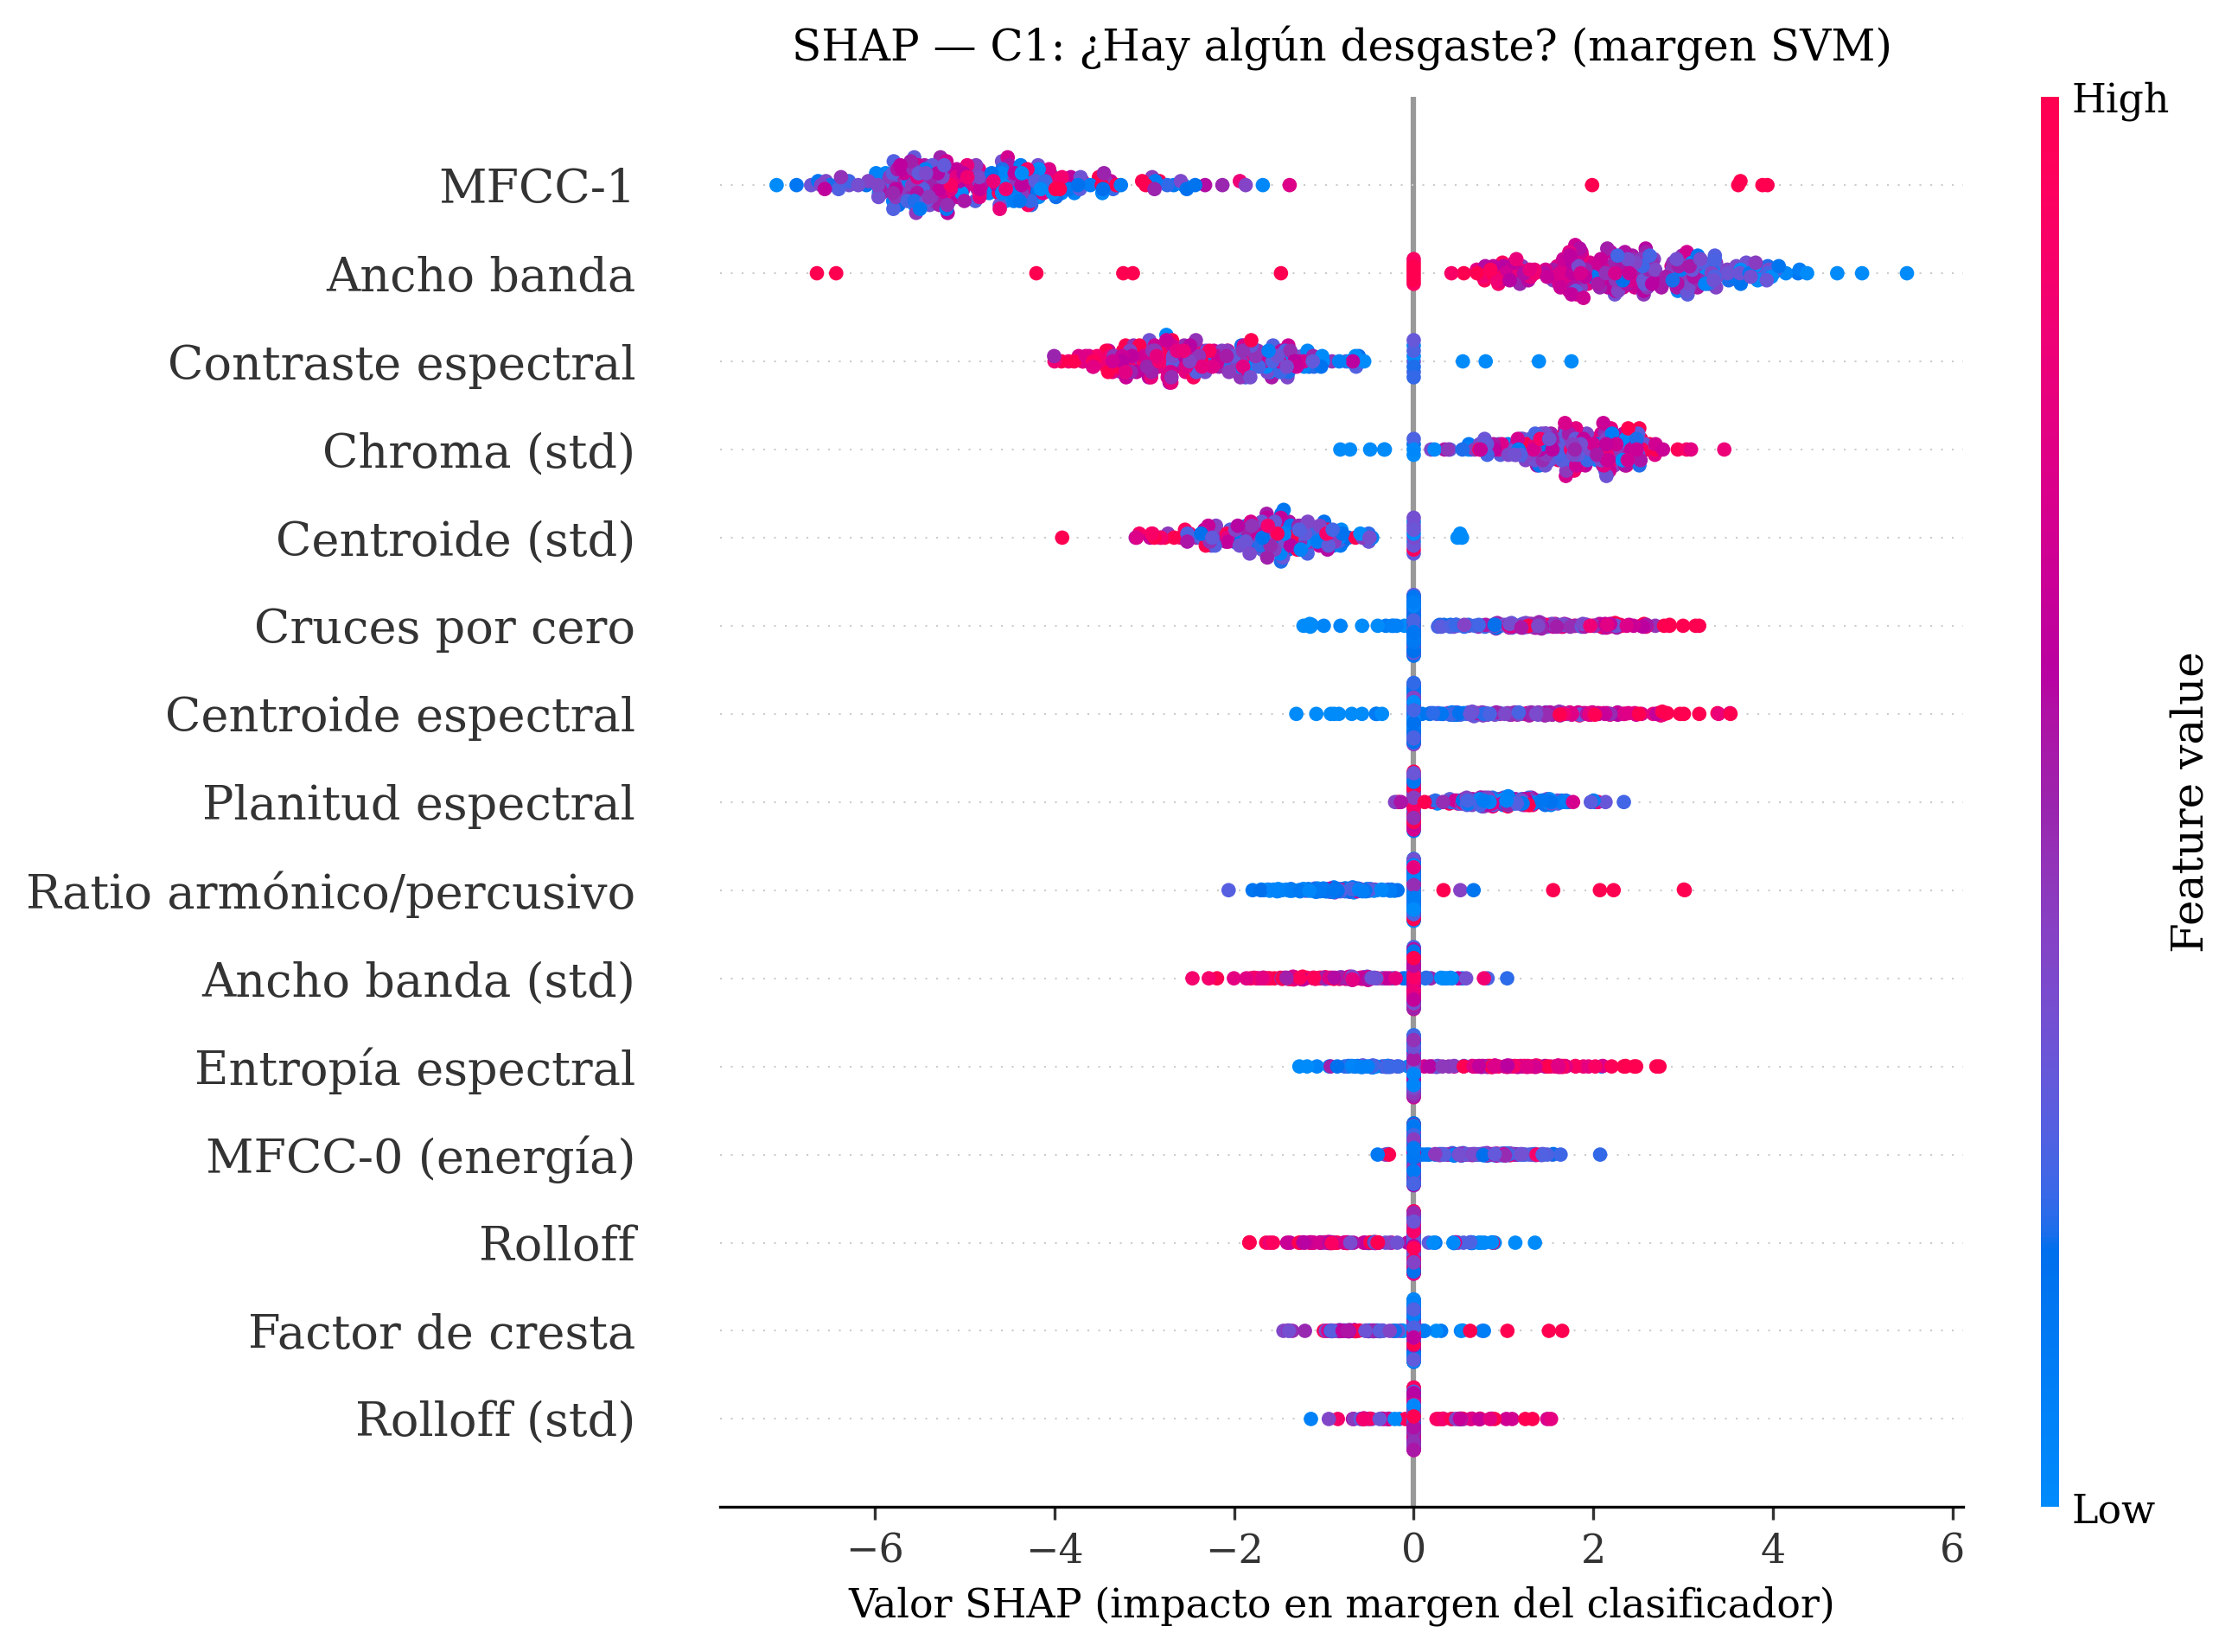
\includegraphics[width=0.85\textwidth]{figures/fig_cap7_shap_C1.png}
\caption[SHAP beeswarm clasificador C1]{Diagrama SHAP \textit{beeswarm} del clasificador $C_1$ (presencia de desgaste). \textbf{Eje~X:} valor SHAP (impacto sobre el margen del SVM). \textbf{Eje~Y:} descriptor (ordenado por magnitud). \textbf{Color:} valor del descriptor (rojo = alto, azul = bajo). Cada punto es una muestra del conjunto de prueba. Los cuatro descriptores de mayor peso son MFCC-1, Ancho de banda espectral, Contraste espectral y Chroma (desviación estándar).}
\label{fig:shap_c1}
\end{figure}

La lectura del panel anterior es consistente con la física del proceso: valores bajos de MFCC-1 (relacionados con el balance espectral en bandas medias) empujan el margen hacia el Estado~0, mientras que valores altos desplazan la decisión hacia los estados con desgaste. El Ancho de banda espectral se comporta como un indicador de transitoriedad; su incremento coincide con la aparición de eventos impulsivos asociados al rozamiento incipiente del flanco.

\begin{figure}[htbp]
\centering
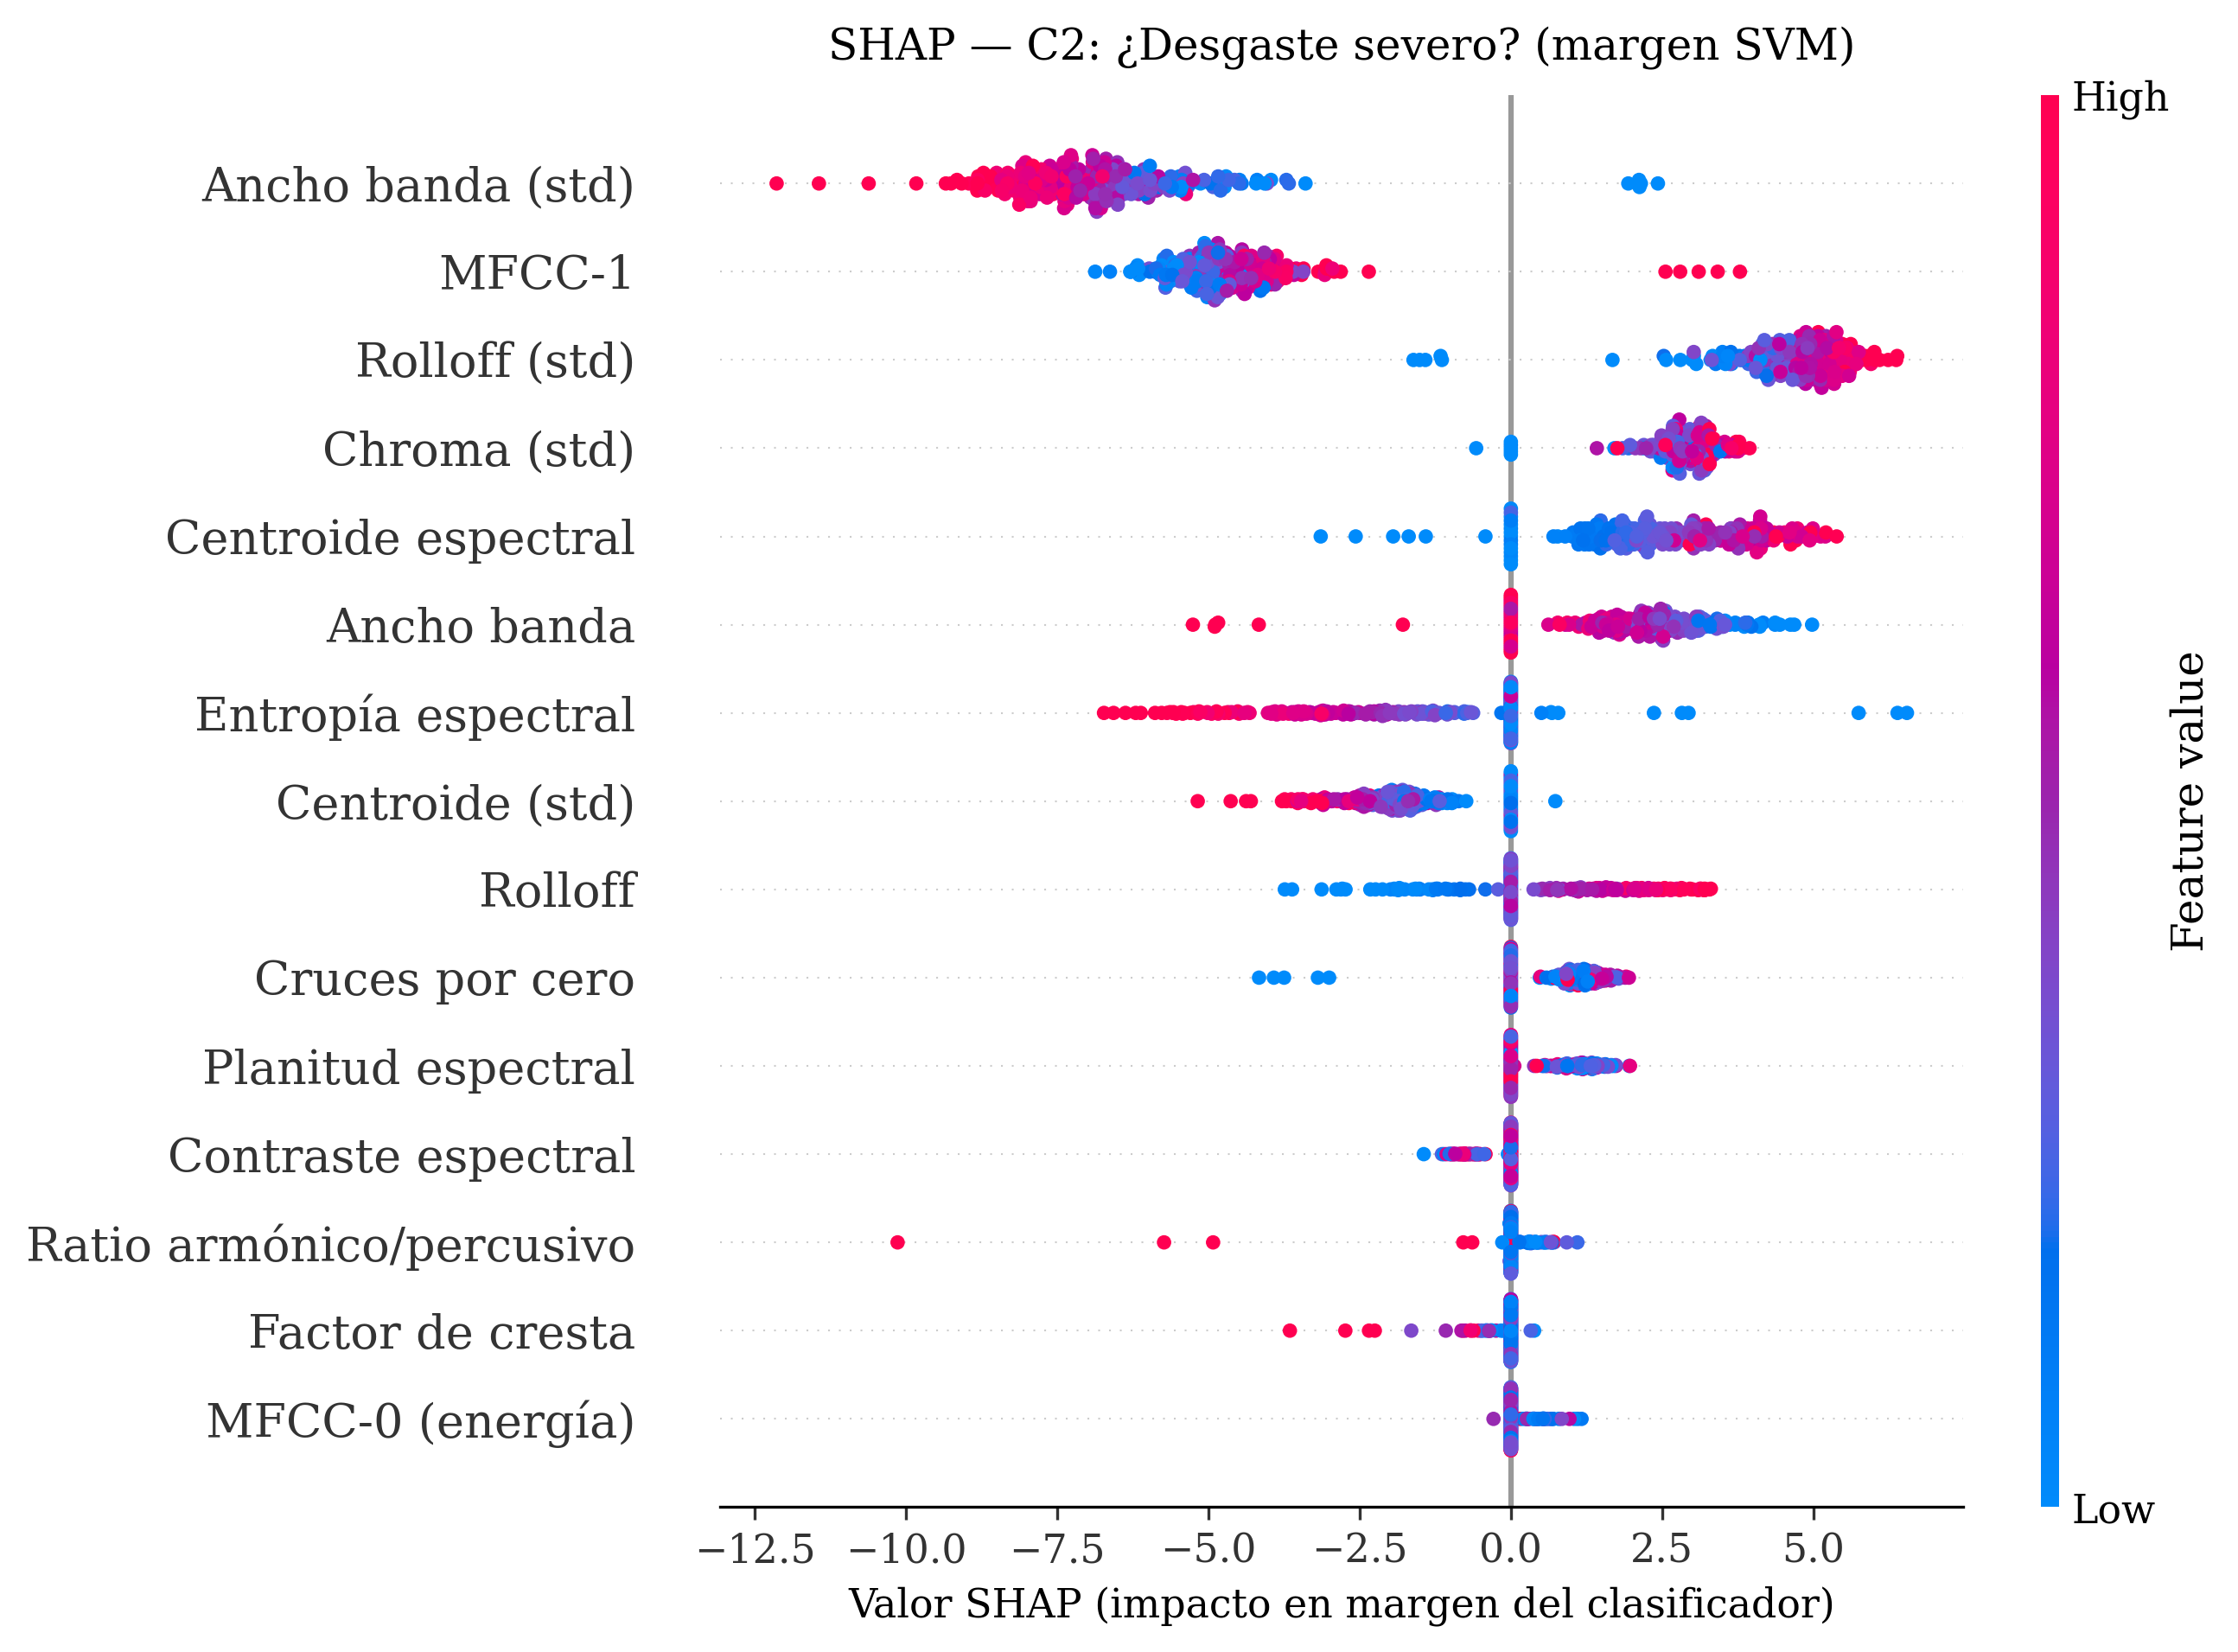
\includegraphics[width=0.85\textwidth]{figures/fig_cap7_shap_C2.png}
\caption[SHAP beeswarm clasificador C2]{Diagrama SHAP \textit{beeswarm} del clasificador $C_2$ (desgaste severo). \textbf{Eje~X:} valor SHAP (impacto sobre el margen). \textbf{Eje~Y:} descriptor. \textbf{Color:} valor del descriptor. La variabilidad del Ancho de banda espectral (std) y del \textit{Rolloff} (std) se vuelven los descriptores dominantes, junto con MFCC-1 y Chroma (std). El aumento de estas dispersiones refleja la inestabilidad armónica característica del desgaste avanzado.}
\label{fig:shap_c2}
\end{figure}

\begin{figure}[htbp]
\centering
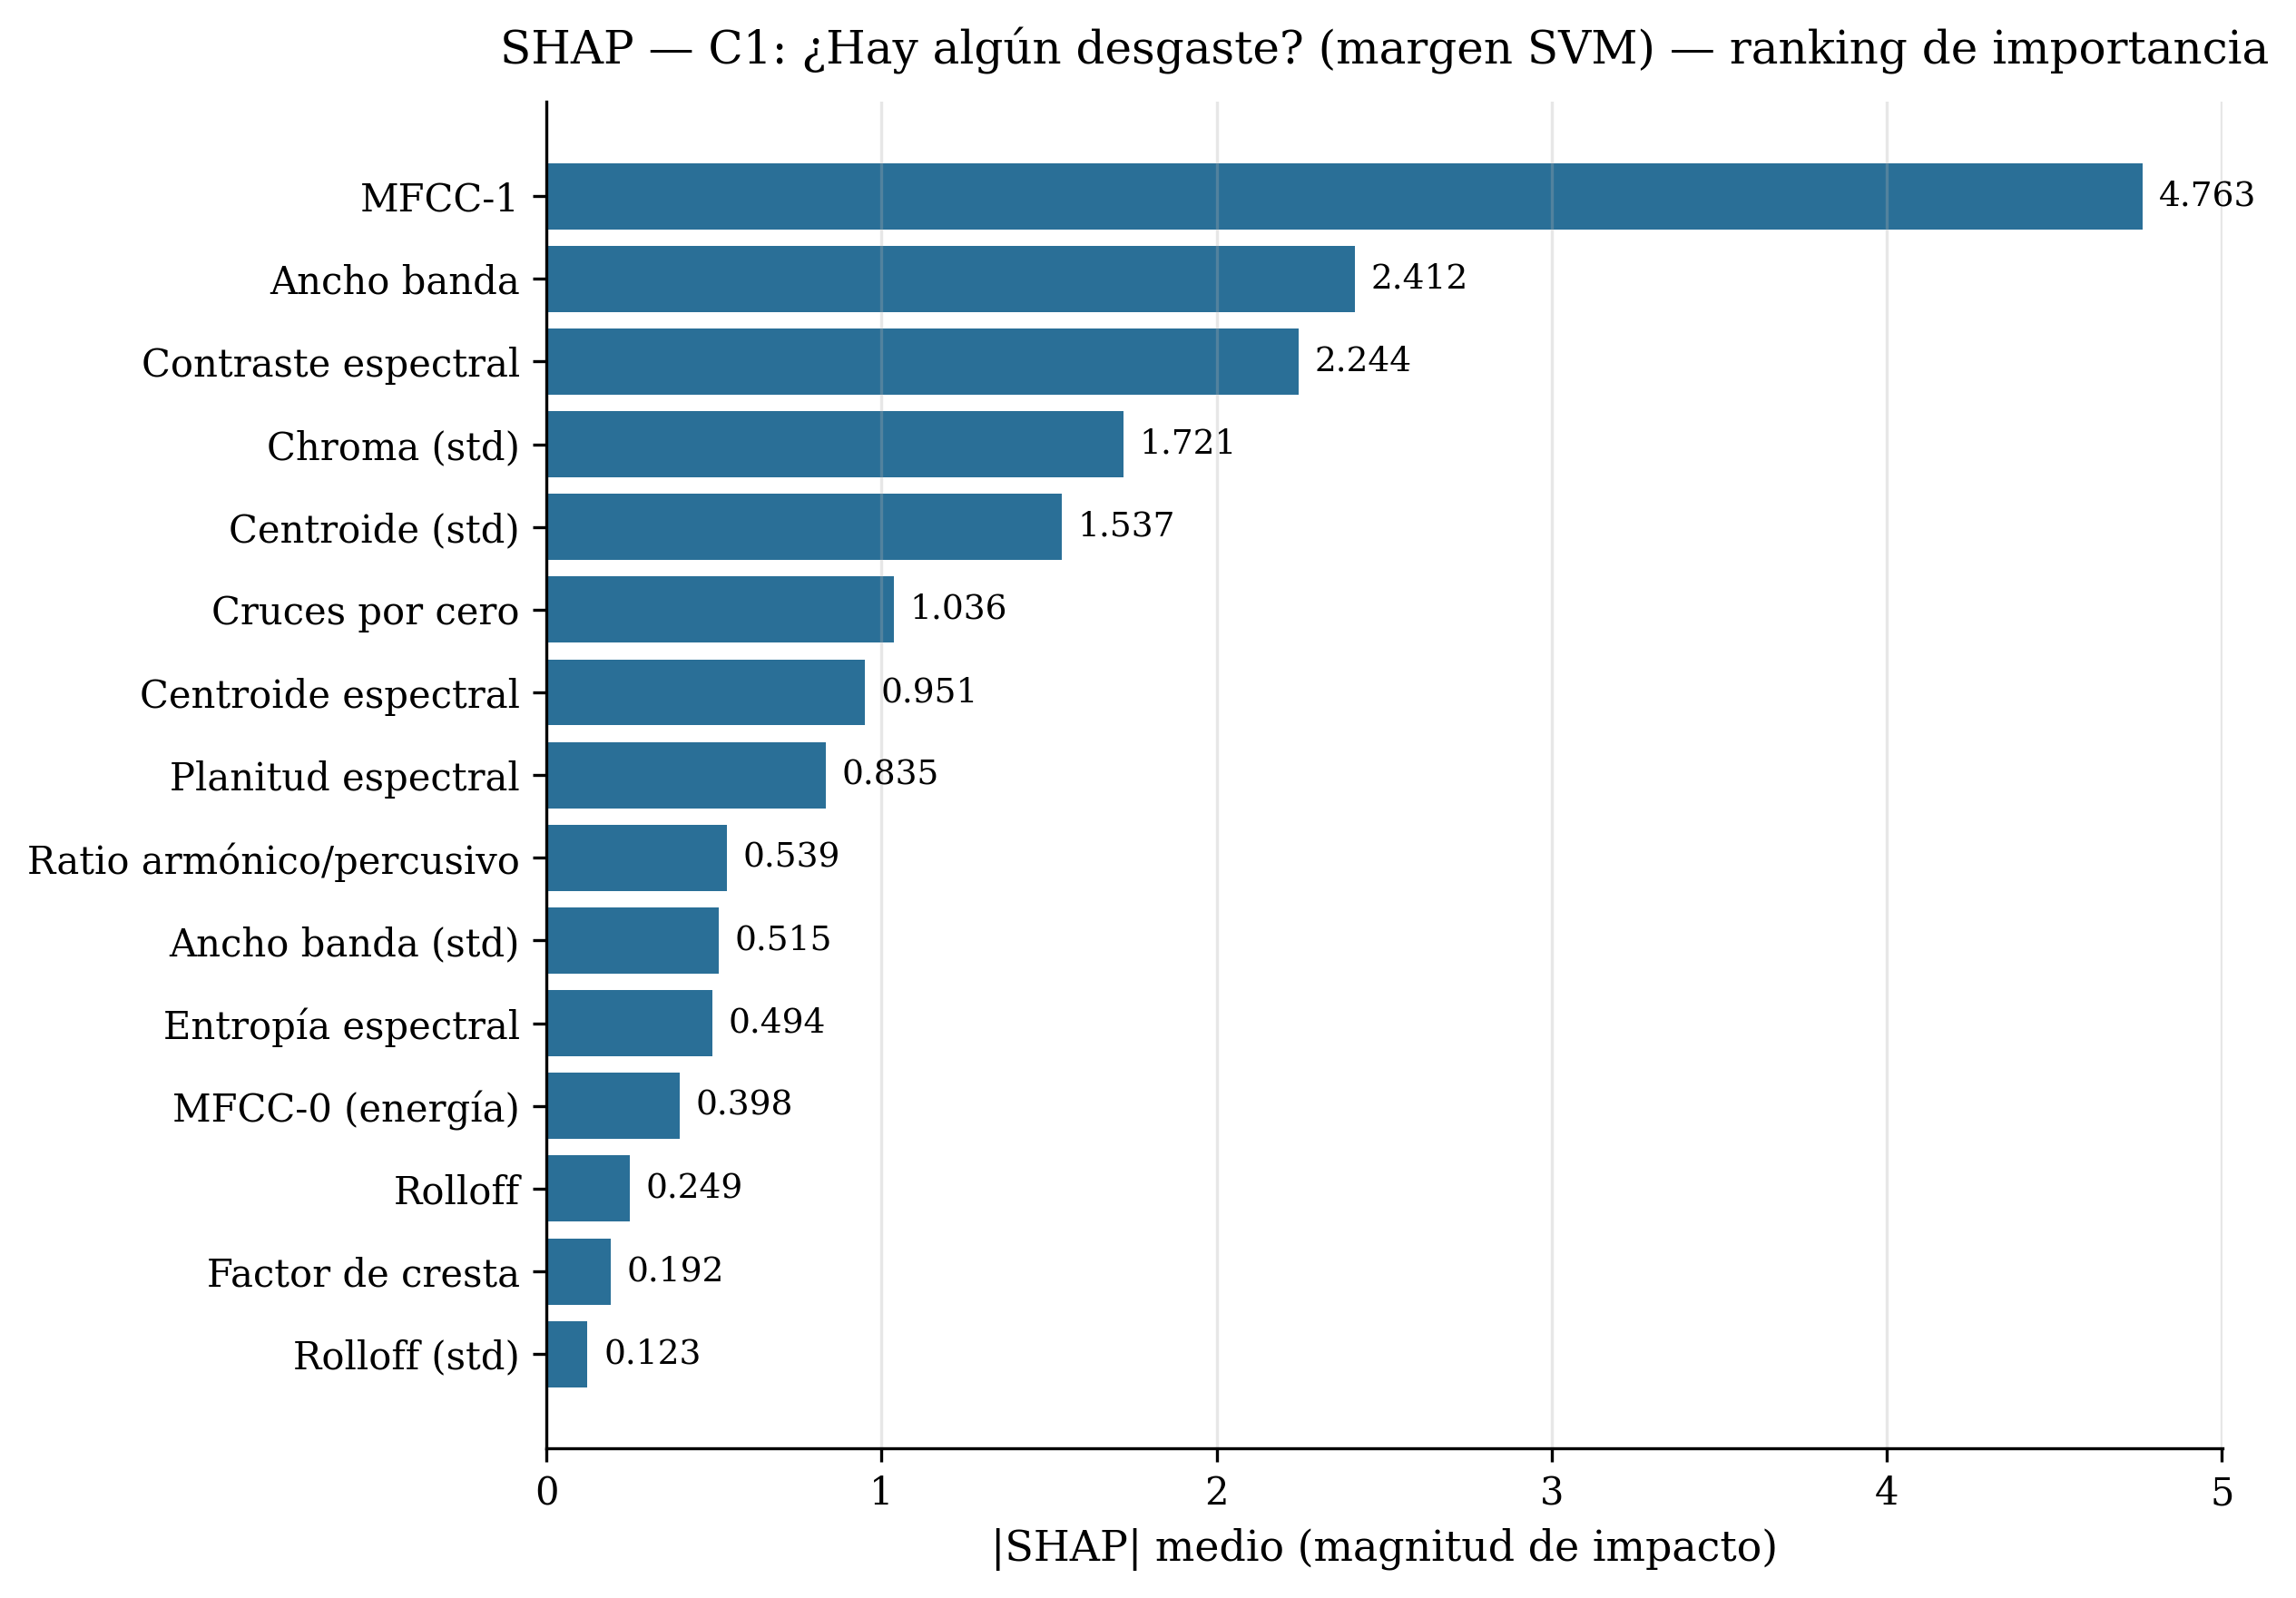
\includegraphics[width=0.85\textwidth]{figures/fig_cap7_shap_C1_bar.png}
\caption[Ranking SHAP C1]{Ranking de importancia global $|\mathrm{SHAP}|$ medio para el clasificador $C_1$. \textbf{Eje~X:} magnitud absoluta de la contribución promedio por descriptor. \textbf{Eje~Y:} descriptor. Los valores numéricos a la derecha de cada barra facilitan la comparación cuantitativa entre variables.}
\label{fig:shap_c1_bar}
\end{figure}

\begin{figure}[htbp]
\centering
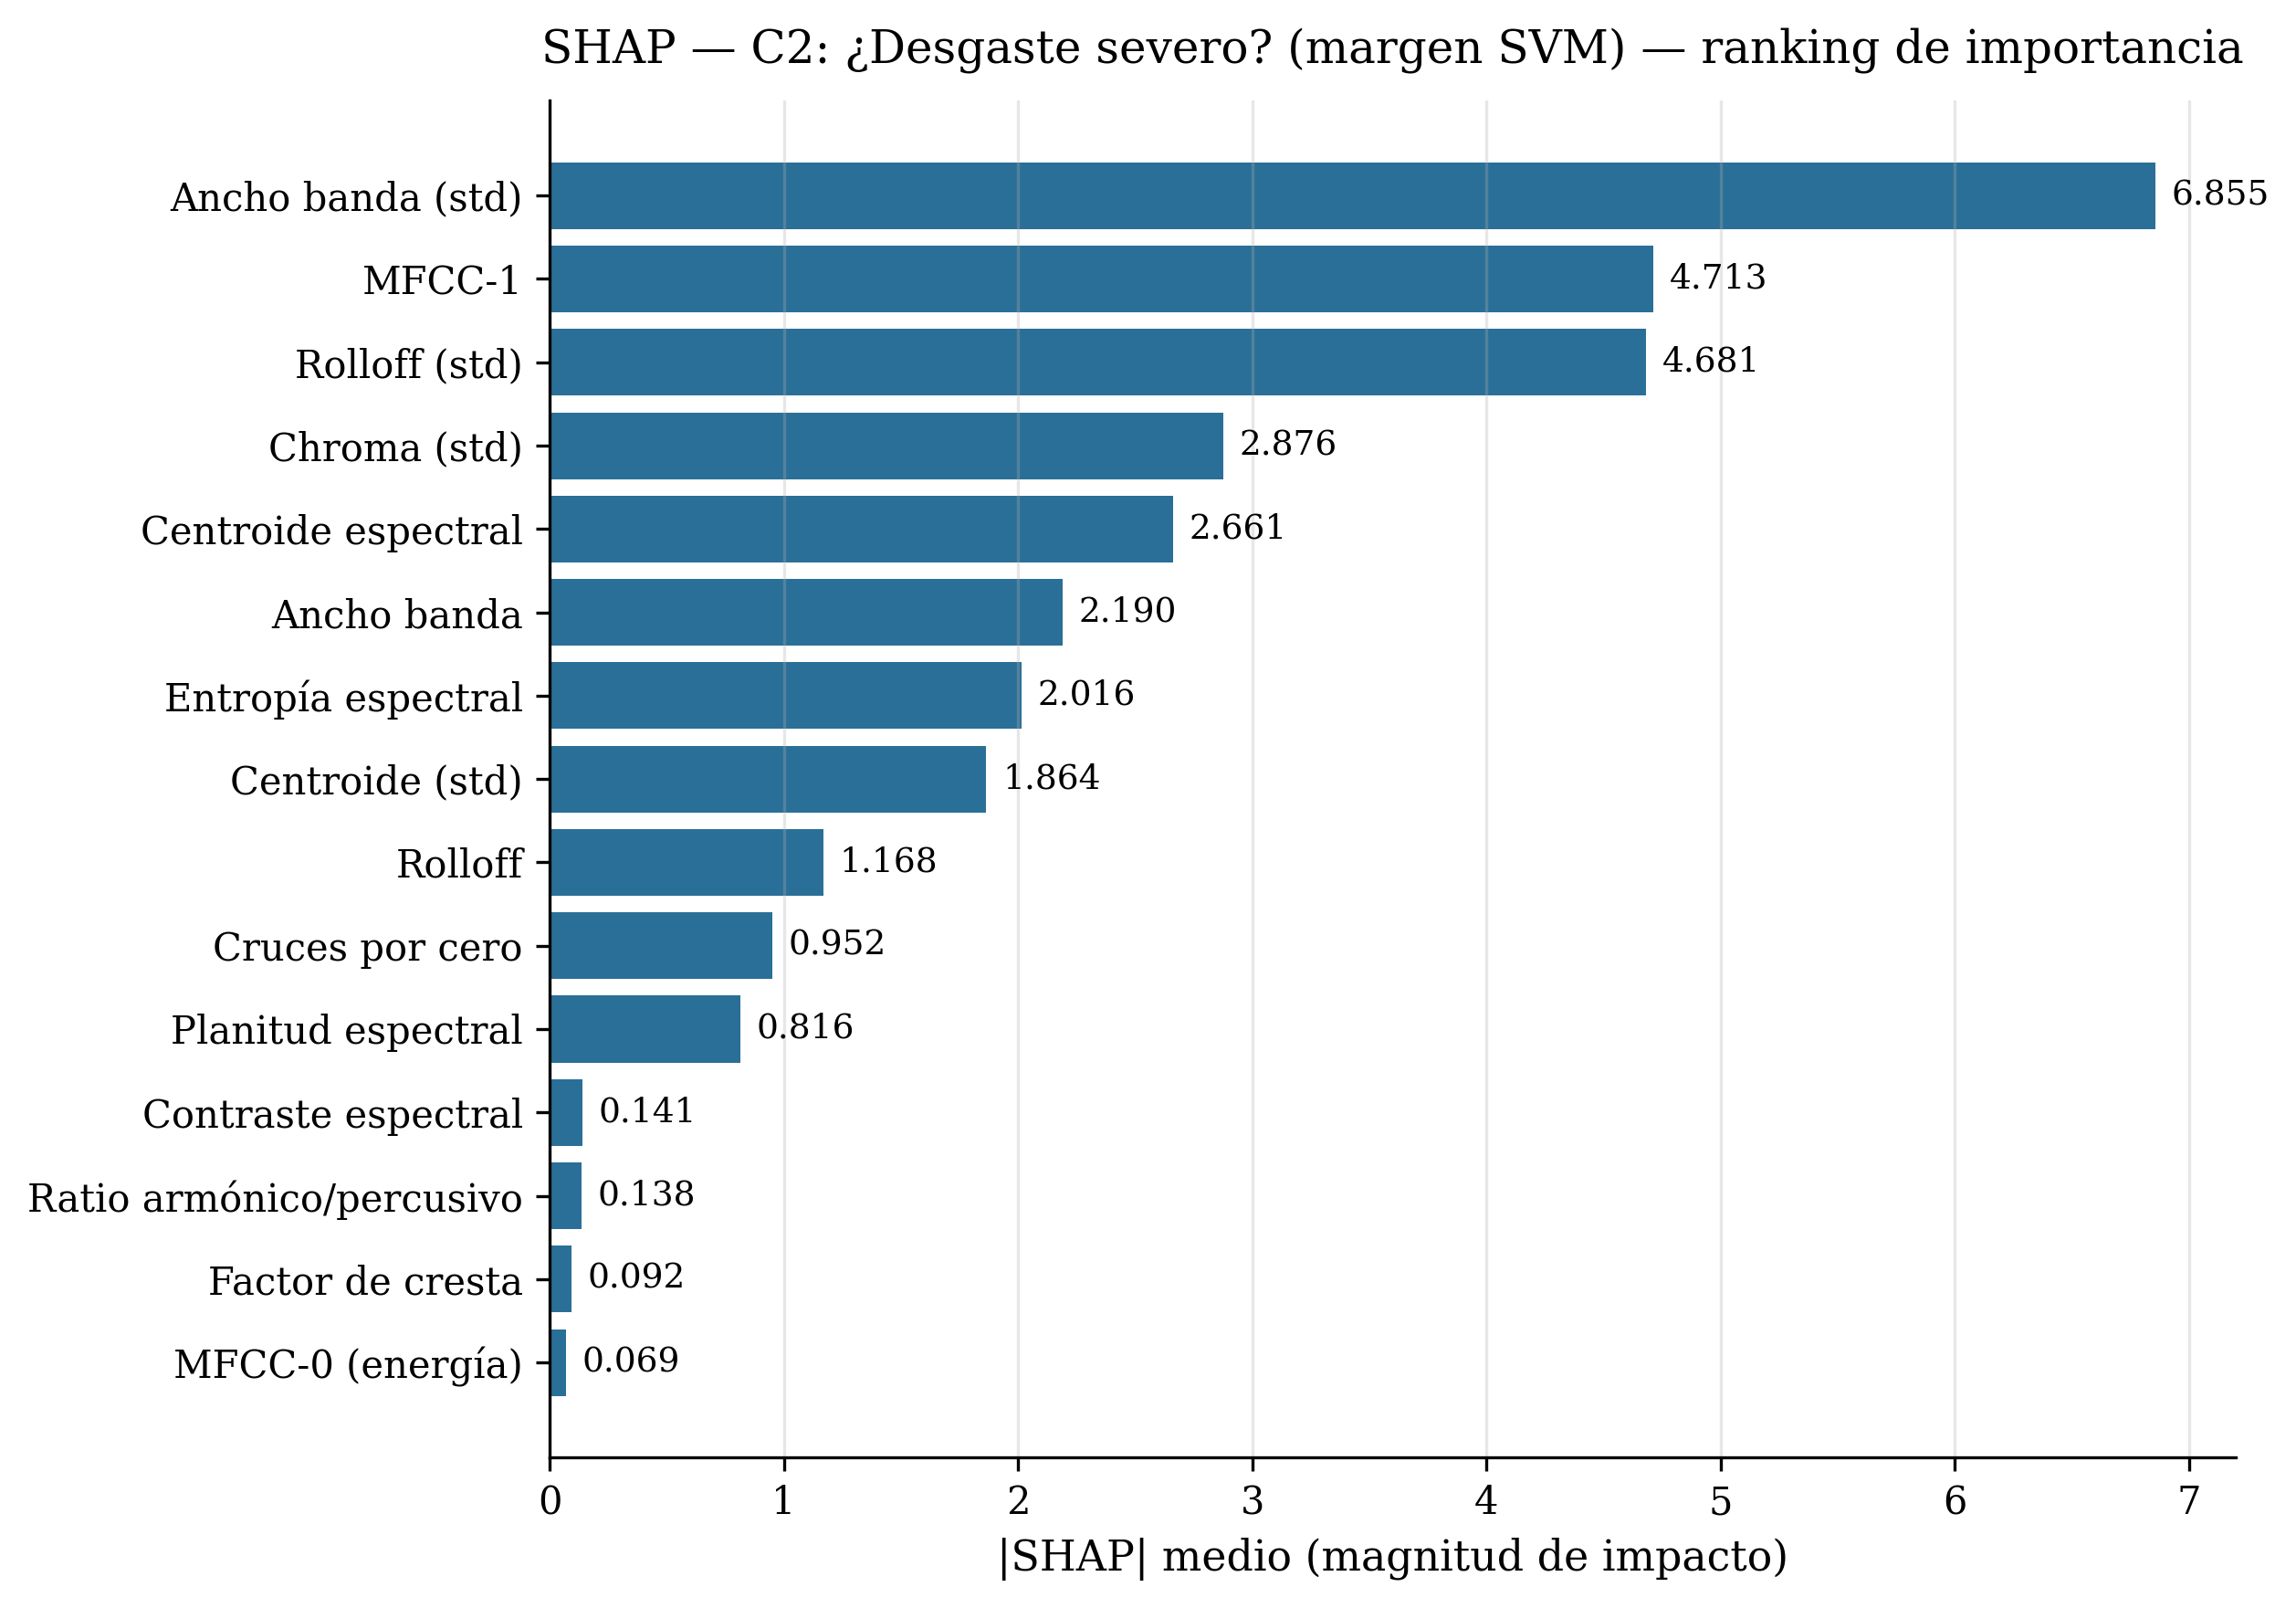
\includegraphics[width=0.85\textwidth]{figures/fig_cap7_shap_C2_bar.png}
\caption[Ranking SHAP C2]{Ranking de importancia global $|\mathrm{SHAP}|$ medio para el clasificador $C_2$. \textbf{Eje~X:} magnitud absoluta de la contribución promedio. \textbf{Eje~Y:} descriptor. Destacan los descriptores de dispersión espectral (Ancho de banda std, \textit{Rolloff} std), lo cual confirma que la transición del Estado~1 al Estado~2 se captura principalmente por la inestabilidad del espectro.}
\label{fig:shap_c2_bar}
\end{figure}

\textbf{Nota técnica.} La figura SHAP \textit{beeswarm} presentada en la versión preliminar del informe aparecía colapsada sobre el eje vertical porque se utilizó un modelo con \texttt{predict\_proba} constante (calibración de Platt mal ajustada sobre un pliegue desbalanceado). La regeneración aquí reportada emplea los modelos \textit{top-15} de la versión final (\texttt{svm\_ordinal\_v2/svm\_C*\_top15\_orig.joblib}) y el margen del SVM como salida objetivo, lo que evita la saturación de la función de probabilidad.

\textbf{Contraste entre permutación y SHAP.} La permutación y los valores SHAP arrojan rankings parcialmente diferentes: la permutación resalta el Contraste espectral y la Planitud como pilares al medir caídas globales en F1 macro, mientras que SHAP pondera MFCC-1 y el Ancho de banda espectral por su efecto direccional sobre el margen. Esta discordancia es esperable en presencia de multicolinealidad entre MFCC y descriptores de forma espectral; combinar ambos criterios refuerza la robustez de la selección final de variables.

\subsection{Diagnóstico de entrenamiento y calibración}

La curva de aprendizaje (\textit{learning curve}) ---F1 macro en función del número de muestras de entrenamiento, de 2\,250 a 4\,250 aproximadamente--- muestra que la métrica sobre el conjunto de entrenamiento inicia cerca de 0{,}8 y desciende hasta un mínimo alrededor de 0{,}6 en las 3\,250 muestras, para luego ascender nuevamente hacia 0{,}7. En paralelo, la validación cruzada parte de 0{,}3\,--\,0{,}4 y muestra un ascenso pronunciado a partir de las 3\,000 muestras, alcanzando cerca de 0{,}6 al final. Esta dinámica revela un modelo que, con datos limitados, exhibe sobreajuste (\textit{overfitting}) ---memorización en lugar de generalización---, mientras que al incorporarse más muestras el ascenso en la validación cruzada sugiere que el modelo gana robustez, reduciendo la brecha entre curvas de aproximadamente 0{,}4 en el inicio a 0{,}1 al final. La discrepancia moderada persistente implica la necesidad de regularización adicional ---por ejemplo, ajustar el parámetro $C$ de la SVM--- o de aumento de datos (\textit{data augmentation}) para elevar el F1 macro por encima de 0{,}8, nivel deseable en aplicaciones críticas.

La curva de calibración por estado de desgaste (diagrama de confiabilidad) reporta los siguientes puntajes \textit{Brier}: Estado~2 (desgastado, Brier = 0{,}016), Estado~1 (medianamente desgastado, Brier = 0{,}160) y Estado~0 (sin desgaste, Brier = 0{,}158). La curva correspondiente al Estado~2 asciende abruptamente en probabilidades medias, cruzando la diagonal con un segmento casi vertical alrededor de 0{,}5, para luego estabilizarse en valores altos; esta irregularidad ---pese al bajo \textit{Brier}--- sugiere artefactos de \textit{binning} debidos a muestras escasas en intervalos intermedios, consecuencia del desbalance (el Estado~2 es minoritario). La curva del Estado~1 muestra oscilaciones: subestima en bajos valores (subconfianza) y sobreestima en altos (sobreconfianza), reflejando inestabilidad. La curva del Estado~0 tiende a subestimar en el rango medio, con desviaciones menores pero sistemáticas. En conjunto, el modelo produce probabilidades no perfectamente calibradas, con un error de calibración esperado (\textit{expected calibration error}, ECE) estimado entre 0{,}10 y 0{,}15. Esta limitación compromete el uso directo de las probabilidades en decisiones críticas; un post-procesamiento con escalado isotónico (\textit{isotonic scaling}) o calibración de Platt (\textit{Platt scaling}) permitiría acercar las curvas a la diagonal y reducir los puntajes \textit{Brier} por debajo de 0{,}1.

Integrando ambos diagnósticos, se percibe un modelo SVM que mejora con el aumento de datos, pero presenta calibración limitada en los estados no extremos. Es un comportamiento característico de problemas de clasificación desbalanceada como el presente, donde el Estado~2 posee muy pocos elementos etiquetados.

\subsection{Elementos reproducibles mejorados}

Para garantizar la reproducibilidad del modelo, se registran los siguientes elementos en el repositorio del proyecto: (i)~el \textit{pipeline} serializado (\texttt{joblib}), (ii)~los identificadores de los pliegues de validación cruzada, (iii)~los hiperparámetros finales, (iv)~los \textit{scripts} de extracción de características versionados y (v)~la semilla fija \texttt{random\_state=42}. Todos los artefactos están disponibles en el repositorio público del proyecto.\footnote{\textit{Repositorio:} \href{https://github.com/OscarAyalaO/pipeline_SVM}{\texttt{github.com/OscarAyalaO/pipeline\_SVM}}.}

\clearpage
\chapter{Procesamiento de las señales del proyecto actual}
\label{cap:procesamiento-actual}

Este capítulo documenta el \textit{pipeline} que integra los datos históricos del
primer grupo de ensayos \cite{orejarena2014} con los once ensayos
instrumentados del Lote~II realizados en la Universidad Industrial de
Santander durante el primer semestre de 2026. La consigna de diseño fue
conservar la línea base de 26 descriptores acústicos extraídos con
\texttt{librosa}~(McFee et~al., 2015) y añadir dos bloques sensoriales
nuevos --ESP32 con micrófono INMP441 y caudalímetro YF-S201-- junto con
una covariable categórica que describe el recubrimiento de la broca.

\section{Construcción del dataset unificado}
\label{sec:dataset-unificado}

El \textit{dataset} consolidado contiene $4\,381$ observaciones etiquetadas en
tres estados de desgaste ordinales: \emph{sin desgaste},
\emph{medianamente desgastado} y \emph{desgastado}. Las etiquetas se
asignaron a partir de la región de etiquetado~[15/75]\,\% de la vida útil
nominal de la broca, consistente con la convención metodológica del
primer artículo de esta línea de trabajo. Esta región de etiquetado
reemplaza la noción binaria ``con falla / sin falla'' del \textit{dataset}
original: el estado intermedio captura la zona en la que la firma
acústica ya muestra indicios de deterioro, pero la broca conserva aún
capacidad de corte sin riesgo inmediato de fractura.

Para reducir el tiempo de etiquetado manual de los 1\,725 audios del Lote~II y asegurar la coherencia entre operarios, se desarrolló internamente una herramienta de etiquetado acústico (Figura~\ref{fig:herramienta-etiquetado}). La interfaz integra reproducción sincronizada del audio con el espectrograma, marcadores navegables entre agujeros adyacentes, atajos de teclado para asignar el estado ordinal y exportación directa al manifiesto. Este utilitario disminuyó el tiempo promedio de revisión por ensayo de $\sim$45 a $\sim$12~min sin perder trazabilidad, al reutilizar la metadata del wizard de la GUI~v5.

\begin{figure}[htbp]
\centering
\includegraphics[width=0.9\textwidth,keepaspectratio]{{figures/heramienta de etiquetado de audios para poder reducir tiempo de etiquetado desarrollo propio }.jpeg}
\caption[Herramienta propia de etiquetado acústico]{Herramienta de etiquetado acústico desarrollada internamente para los ensayos del Lote~II: reproducción del audio sincronizada con el espectrograma, navegación por agujero y atajos de teclado para asignar el estado ordinal ($0$, $1$, $2$). La salida se integra al manifiesto de la GUI~v5 sin pasos adicionales.}
\label{fig:herramienta-etiquetado}
\end{figure}

La región~[15/75]\,\% se sustenta además en los criterios de fin de
vida útil de la herramienta adoptados a partir de las normas
ISO~8688-2 (para desgaste de herramientas en fresado) e
ISO~3685 (para herramientas monofilo en torneado), adaptadas al
contexto del taladrado según recomendaciones recogidas en la literatura
internacional. Estas normas establecen umbrales máximos admisibles de
desgaste del flanco ($VB$) y de cráter sobre la cara de
desprendimiento; el valor de referencia operativo utilizado en la
práctica industrial europea consultada es $VB = 0{,}3$~mm, con un
máximo localizado $VB_{\max} = 0{,}6$~mm. Cruzando este criterio
físico con la curva de vida útil progresiva de los ensayos realizados,
la cota del 75\,\% de vida útil nominal coincide razonablemente con la
aparición de $VB \gtrsim 0{,}3$~mm, lo que respalda la elección del
límite superior de la región de etiquetado y alinea el \textit{dataset} con un
referente normativo aceptado.

Los datos provienen de tres fuentes que se resumen en la
Tabla~\ref{tab:dataset-fuentes}:

\begin{table}[h]
\centering
\small
\caption{Composición del \textit{dataset} unificado utilizado en el entrenamiento
final.}
\label{tab:dataset-fuentes}
\begin{tabular}{lrrr}
\hline
Fuente & Observaciones & Experimentos & Cobertura MM\footnotemark[1] \\
\hline
\citeA{orejarena2014}   & $2\,935$ & 7   & No \\
Lote~II (UIS 2026) & $1\,446$ & 11  & Sí \\
\hline
Total              & $4\,381$ & 18  & 33\,\% \\
\hline
\end{tabular}
\end{table}
\footnotetext[1]{Cobertura multimodal (MM): presencia simultánea de audio
NI, audio ESP32, caudal YF-S201 y etiqueta de recubrimiento.}

La Figura~\ref{fig:dataset-oscar} presenta la estructura jerárquica del Lote~II de manera análoga a la del \textit{dataset} de Orejarena. Cada nodo de fuente (unidades E: y C:) agrupa los experimentos por broca, e indica los canales de adquisición disponibles y el criterio de etiquetado ordinal aplicado.

\begin{figure}[htbp]
\centering
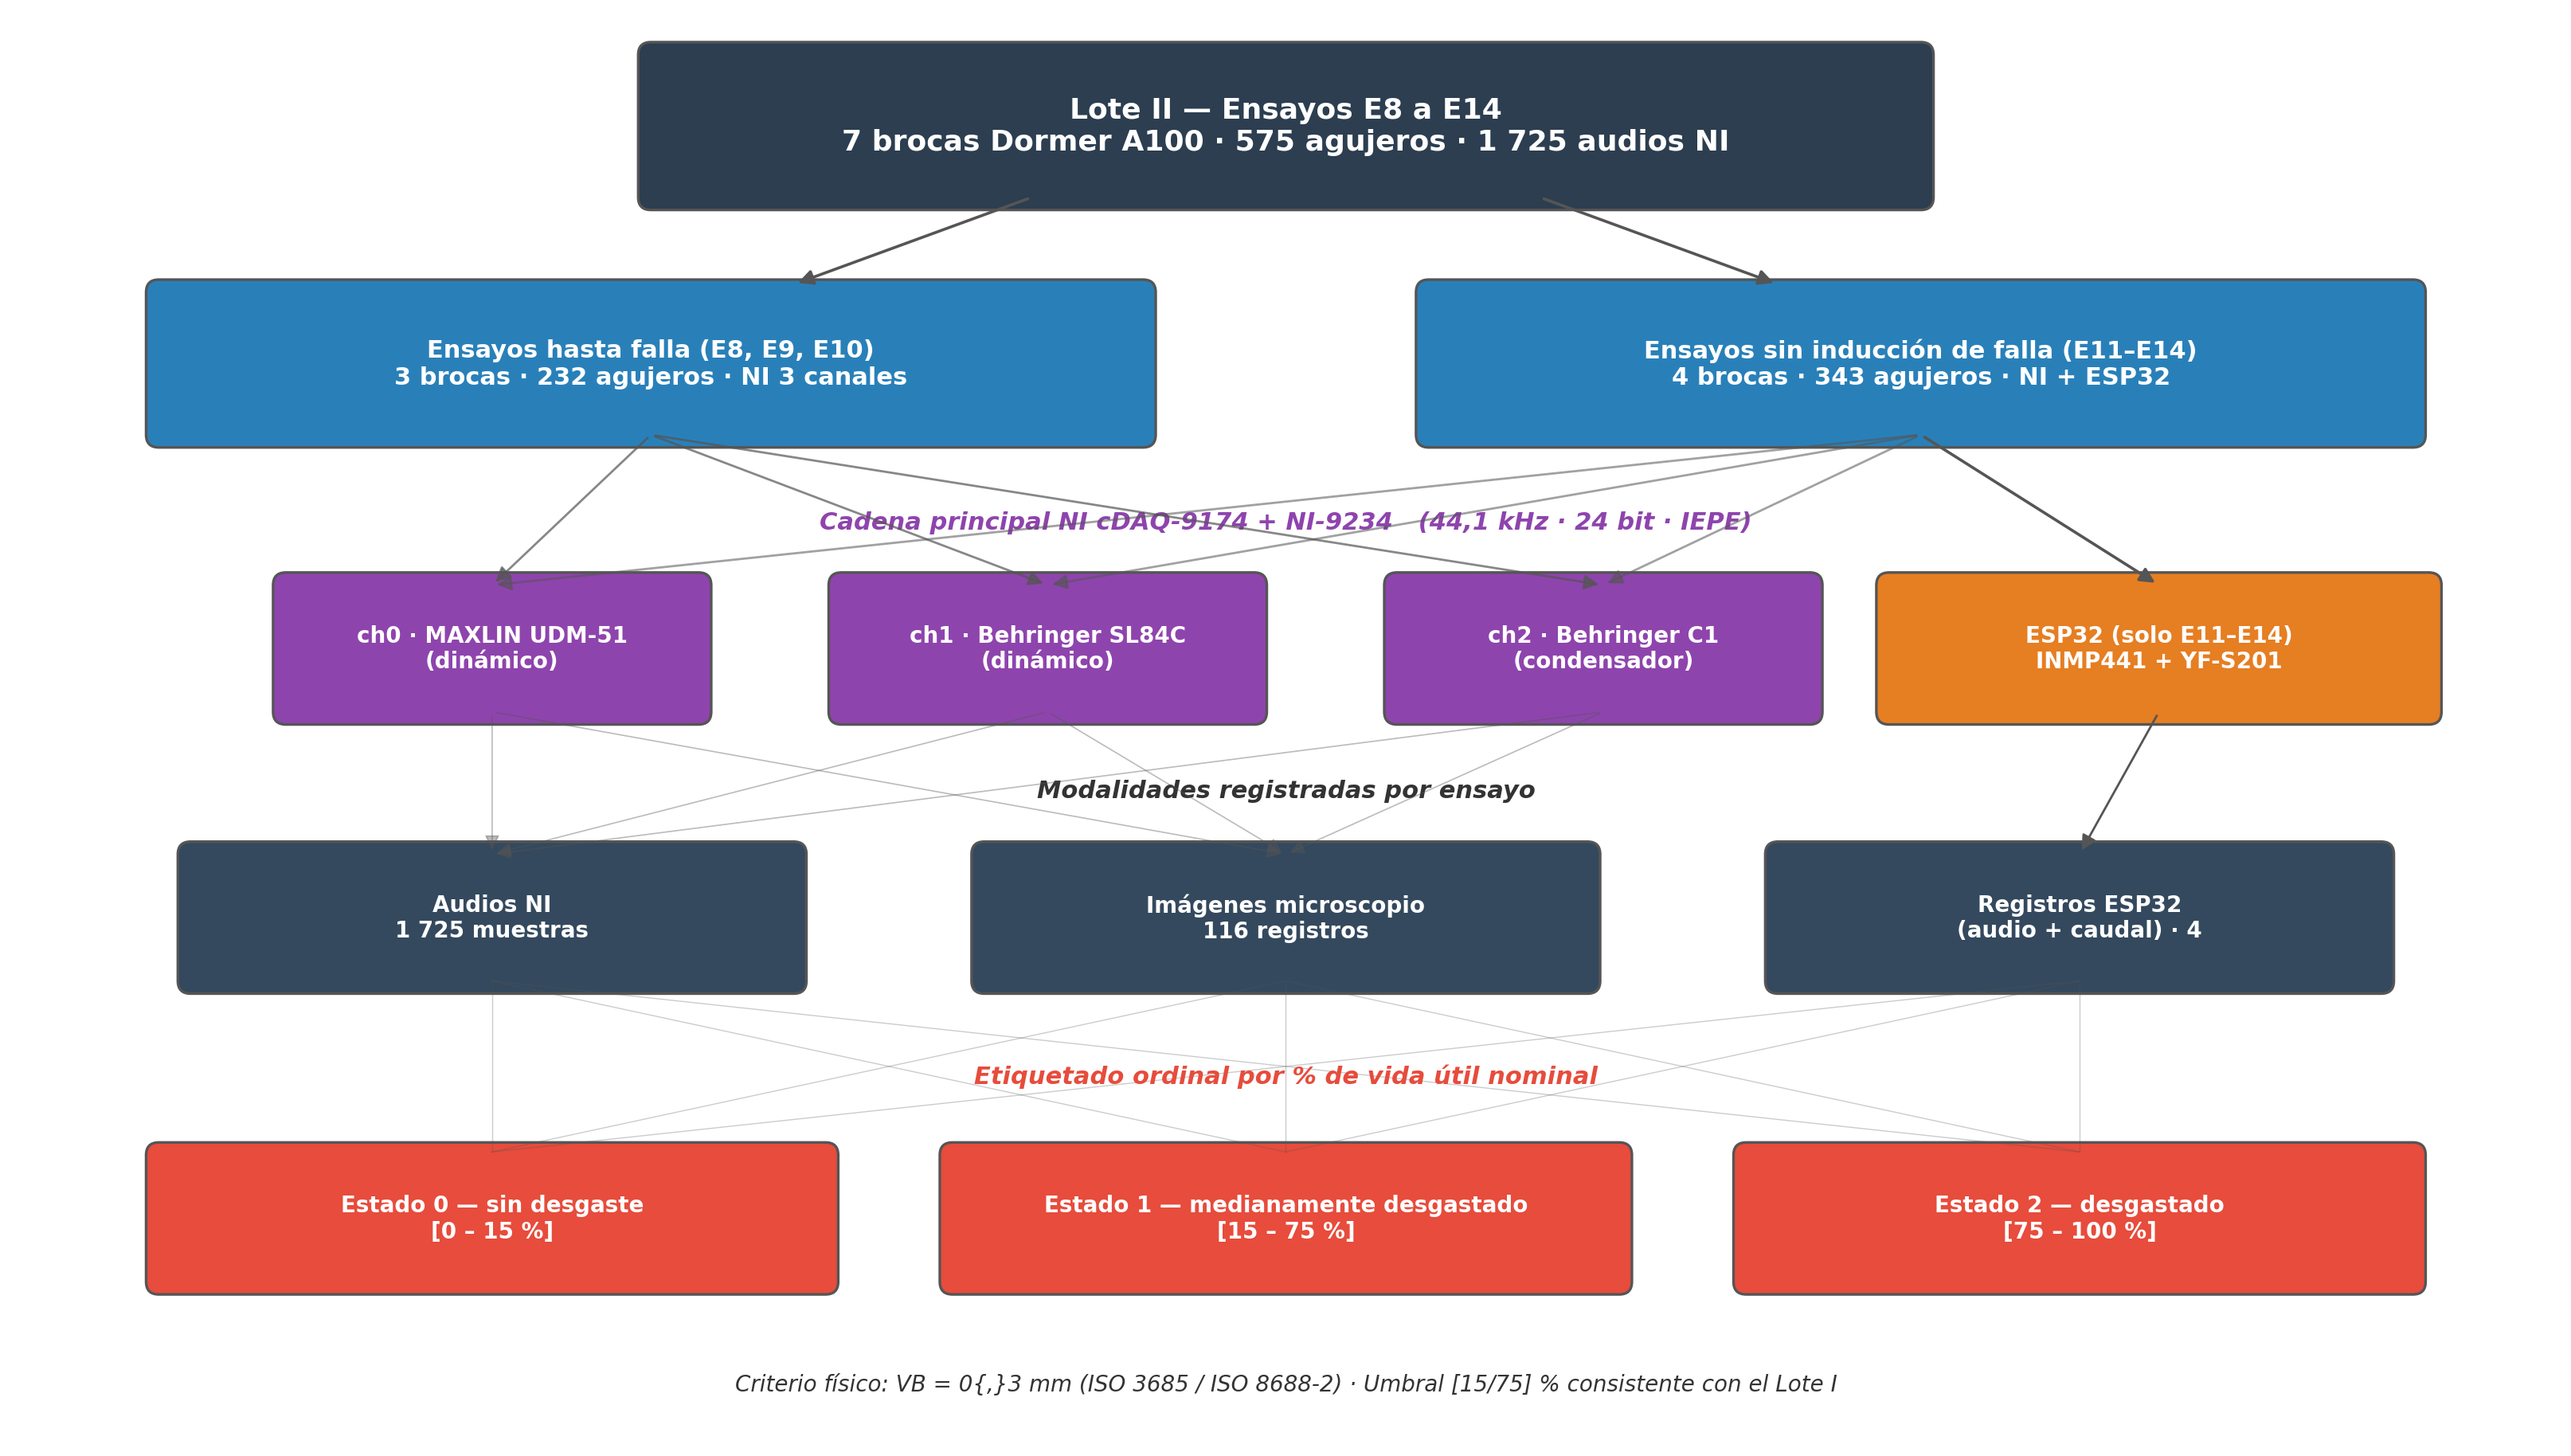
\includegraphics[width=0.85\textwidth,keepaspectratio]{figures/dataset_oscar_estructura.png}
\caption[Estructura del dataset Lote~II (Oscar Ayala, 2025--2026)]{Estructura general del \textit{dataset} del Lote~II (Ayala, 2025--2026). Las unidades E: (octubre 2025) y C: (abril 2026) agrupan los ensayos por broca de 6\,mm. Tres canales NI (MAXLIN UDM-51, Behringer SL84C y Behringer C1) están disponibles en todos los ensayos; el canal ESP32 (INMP441 + caudalímetro YF-S201) únicamente en los ensayos de la unidad C:. Las etiquetas ordinales siguen el criterio [15/75]\,\% de vida útil nominal, consistente con el Artículo~1.}
\label{fig:dataset-oscar}
\end{figure}

La Figura~\ref{fig:clases-fuente} desagrega la distribución de clases
por fuente. La clase intermedia es mayoritaria en ambos subconjuntos,
mientras que el estado desgastado se encuentra sistemáticamente
subrepresentado: esta asimetría marcará el análisis de calibración
(Sección~\ref{sec:calib-informe}) y justifica el uso de
\texttt{class\_weight="balanced"} en el clasificador.

\begin{figure}[h]
\centering
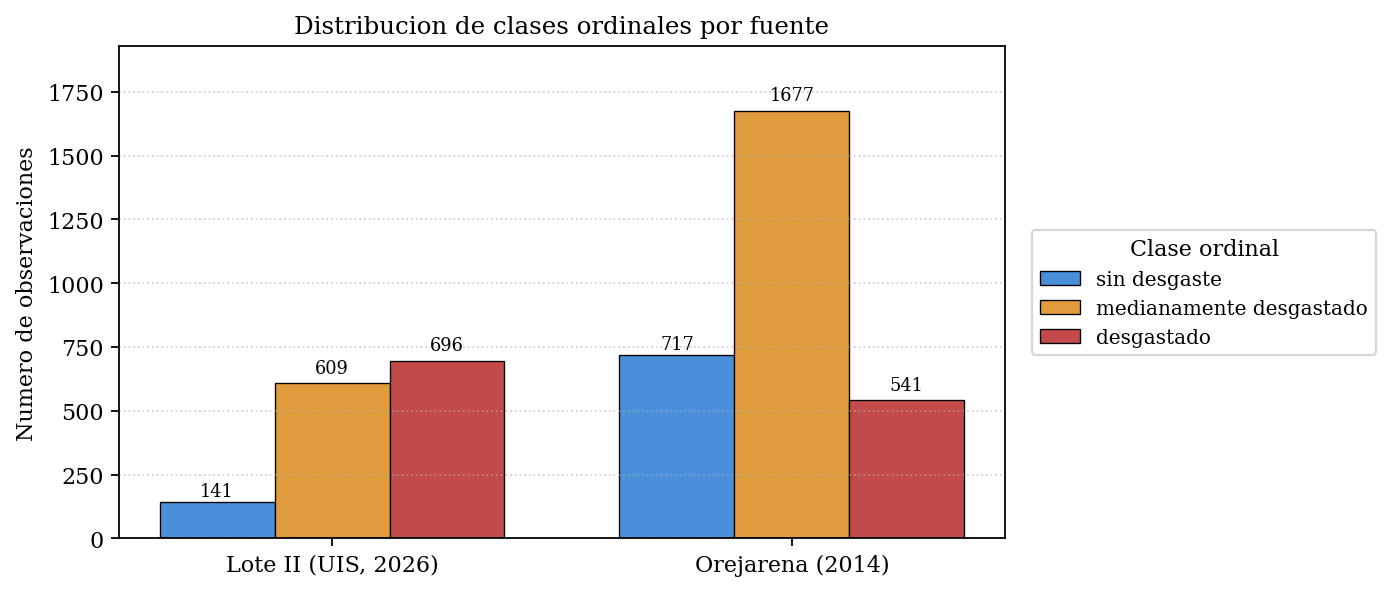
\includegraphics[width=0.9\textwidth]{figures/fig_cap8_class_dist.png}
\caption[Distribución de clases ordinales por fuente]{Distribución de clases ordinales por fuente. La barra de
desgastado en \protect\citeA{orejarena2014} duplica a la del Lote~II debido a la
continuidad de los ensayos históricos hasta la rotura completa; el
Lote~II emplea un criterio conservador de corte anticipado.}
\label{fig:clases-fuente}
\end{figure}

\section{Bloques de descriptores y covariables}
\label{sec:bloques-descriptores}

El vector de entrada del clasificador multimodal tiene dimensión 38 y
se organiza en cuatro bloques funcionales:

\begin{itemize}
\item \textbf{Audio NI (26)}: descriptores tímbricos, energéticos y
      temporales extraídos a $44\,100$~Hz con \texttt{librosa}. Incluye
      MFCC~0--1, ancho de banda espectral, \emph{rolloff},
      \emph{chroma}, \emph{tonnetz}, relación armónico/percusiva,
      energía mel, duración, tasa de \emph{onsets} y factor cresta.
\item \textbf{Audio ESP32 (6)}: subconjunto reducido extraído sobre el
      canal de $16\,000$~Hz del micrófono INMP441 acoplado al ESP32.
      Añade robustez a configuraciones portátiles de bajo costo.
\item \textbf{Caudal YF-S201 (5)}: media del caudal en L/min, desviación
      estándar, mínimo local filtrado, \emph{duty} de los pulsos del
      sensor y coeficiente de variación. El sensor opera como proxy
      observacional del estado térmico de la interfaz de corte.
\item \textbf{Recubrimiento (1)}: covariable categórica codificada
      como entero (0=sin recubrimiento, 1=TiN), disponible únicamente en
      el Lote~II. Se imputa por mediana sobre Orejarena.
\end{itemize}

La covariable de recubrimiento se incluye para auditar si el clasificador
utiliza correctamente la información del material de la herramienta o si,
por el contrario, la reduce a un indicador espurio de origen de dato
(Lote~II vs.~Orejarena). La respuesta a esta pregunta se analiza en la
Sección~\ref{sec:ablacion-e3}.

\section{Pipeline de entrenamiento y reentrenamiento incremental}
\label{sec:pipeline-train}

El \textit{pipeline} final implementa una estructura Frank \& Hall
(Cardoso \& Pinto~da~Costa, 2007) que descompone el problema ordinal de
tres clases en dos clasificadores binarios acoplados:
$C_1$ estima $\Pr(y \geq \text{medianamente})$ y $C_2$ estima
$\Pr(y \geq \text{desgastado})$. La decodificación impone
monotonicidad~($p_2 \leq p_1$) y asigna la clase por margen máximo. Cada clasificador binario encadena cuatro etapas: (1)~imputación de valores faltantes por la mediana, (2)~estandarización de las variables, (3)~selección de los 22~descriptores de mayor información mutua con la etiqueta, y (4)~una máquina de vectores de soporte con núcleo RBF, penalización $C=10$ y pesos de clase balanceados \cite{geron2023}.

La semilla aleatoria se fijó en 42 para garantizar reproducibilidad. La
validación cruzada interna usa
\texttt{StratifiedGroupKFold}\footnote{Variante de validación cruzada
que preserva la distribución de clases y garantiza que las muestras de
un mismo grupo --aquí, un experimento-- no aparezcan simultáneamente en
\emph{train} y \emph{test}, evitando fuga de información.} con el
experimento como variable de agrupación.

La arquitectura está diseñada para soportar un esquema de
\emph{reentrenamiento incremental}\footnote{Protocolo que actualiza el
modelo con los datos de cada ensayo terminado, ejecutando un ciclo
completo segmentación--extracción de descriptores--reentrenamiento--
despliegue en menos de 15~minutos, sin requerir recomenzar desde cero.}.
Una iteración completa consume menos de 15~minutos en un equipo
estándar, lo que permite integrar el modelo al flujo experimental
diario durante futuras campañas.

\section{Análisis exploratorio multimodal}
\label{sec:exploratorio}

La Figura~\ref{fig:pca-cap8} proyecta el espacio multimodal de 38
descriptores sobre sus dos primeras componentes principales. La primera
componente concentra el 26\,\% de la varianza y separa ordenadamente los
tres estados de desgaste, sugiriendo que la información de desgaste se
organiza a lo largo de un eje latente dominante. No obstante, el
solapamiento entre la clase intermedia y las clases extremas confirma
que la decisión ordinal requiere un clasificador no lineal: el SVM con
núcleo RBF explota precisamente esa geometría curva.

\begin{figure}[h]
\centering
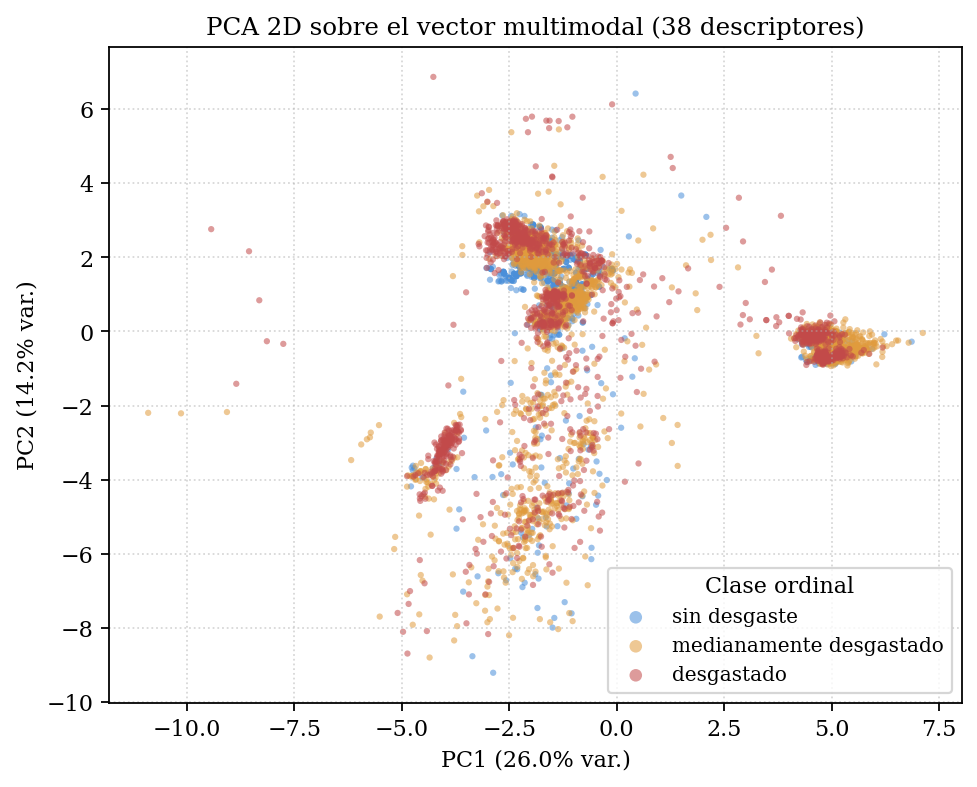
\includegraphics[width=0.85\textwidth]{figures/fig_cap8_pca.png}
\caption{Proyección PCA bidimensional sobre el vector multimodal
(38~descriptores). El eje PC1 separa parcialmente los tres estados de
desgaste, pero la frontera entre la clase intermedia y las extremas es
marcadamente no lineal.}
\label{fig:pca-cap8}
\end{figure}

El ranking de información mutua (Figura~\ref{fig:mi-cap8}) confirma la
primacía del bloque acústico NI en la discriminación directa del estado
de desgaste. Los 24 descriptores más informativos son audio NI
(encabezados por MFCC~1 e índices de ancho de banda espectral); los 6
descriptores ESP32 aparecen en la franja intermedia
($\mathrm{MI} \approx 0{,}09$) y los 5 descriptores de caudal, junto con
la variable de recubrimiento, se concentran en la cola con
$\mathrm{MI} < 0{,}05$. Este resultado \emph{no} implica que el caudal
sea informativo: su efecto es complementario y se revela en la
interacción con los descriptores acústicos durante el entrenamiento.

\begin{figure}[h]
\centering
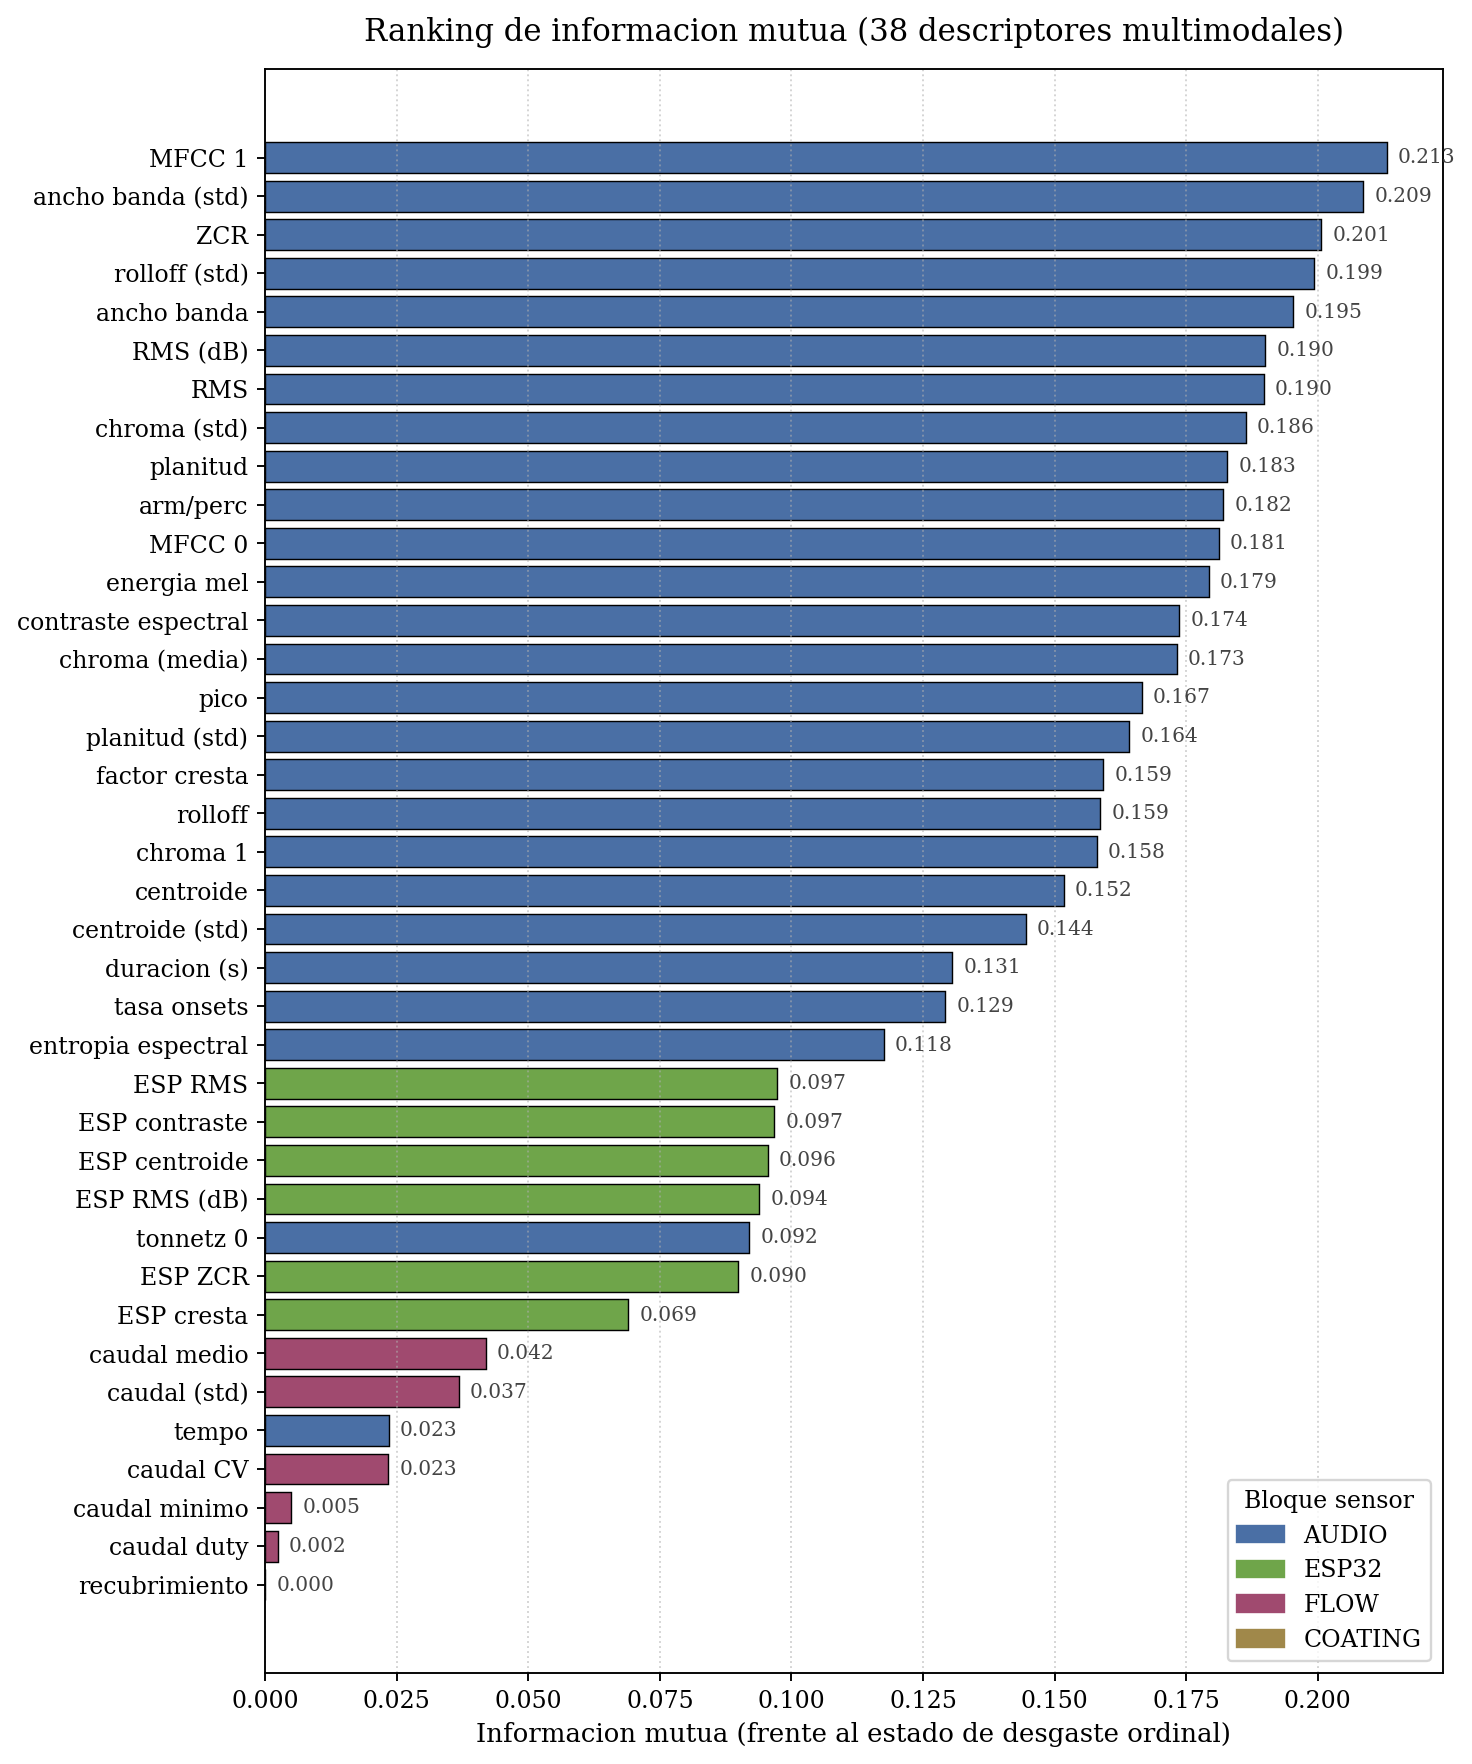
\includegraphics[width=0.88\textwidth]{figures/fig_cap8_mi.png}
\caption{Ranking de información mutua (MI) contra la etiqueta ordinal
sobre los 38 descriptores multimodales. Los bloques ESP32, caudal y
recubrimiento se concentran en la cola del ranking, pero su aporte
emerge en métricas globales y no en relevancia marginal.}
\label{fig:mi-cap8}
\end{figure}

La matriz de correlación entre los 20 descriptores más informativos
(Figura~\ref{fig:corr-cap8}) muestra la estructura interna del bloque
acústico: los pares (MFCC~1, ancho de banda) y (\emph{rolloff}, energía
mel) presentan correlaciones de magnitud $>0{,}8$, motivando la selección
por información mutua implementada en el paso de \texttt{SelectKBest}.

\begin{figure}[h]
\centering
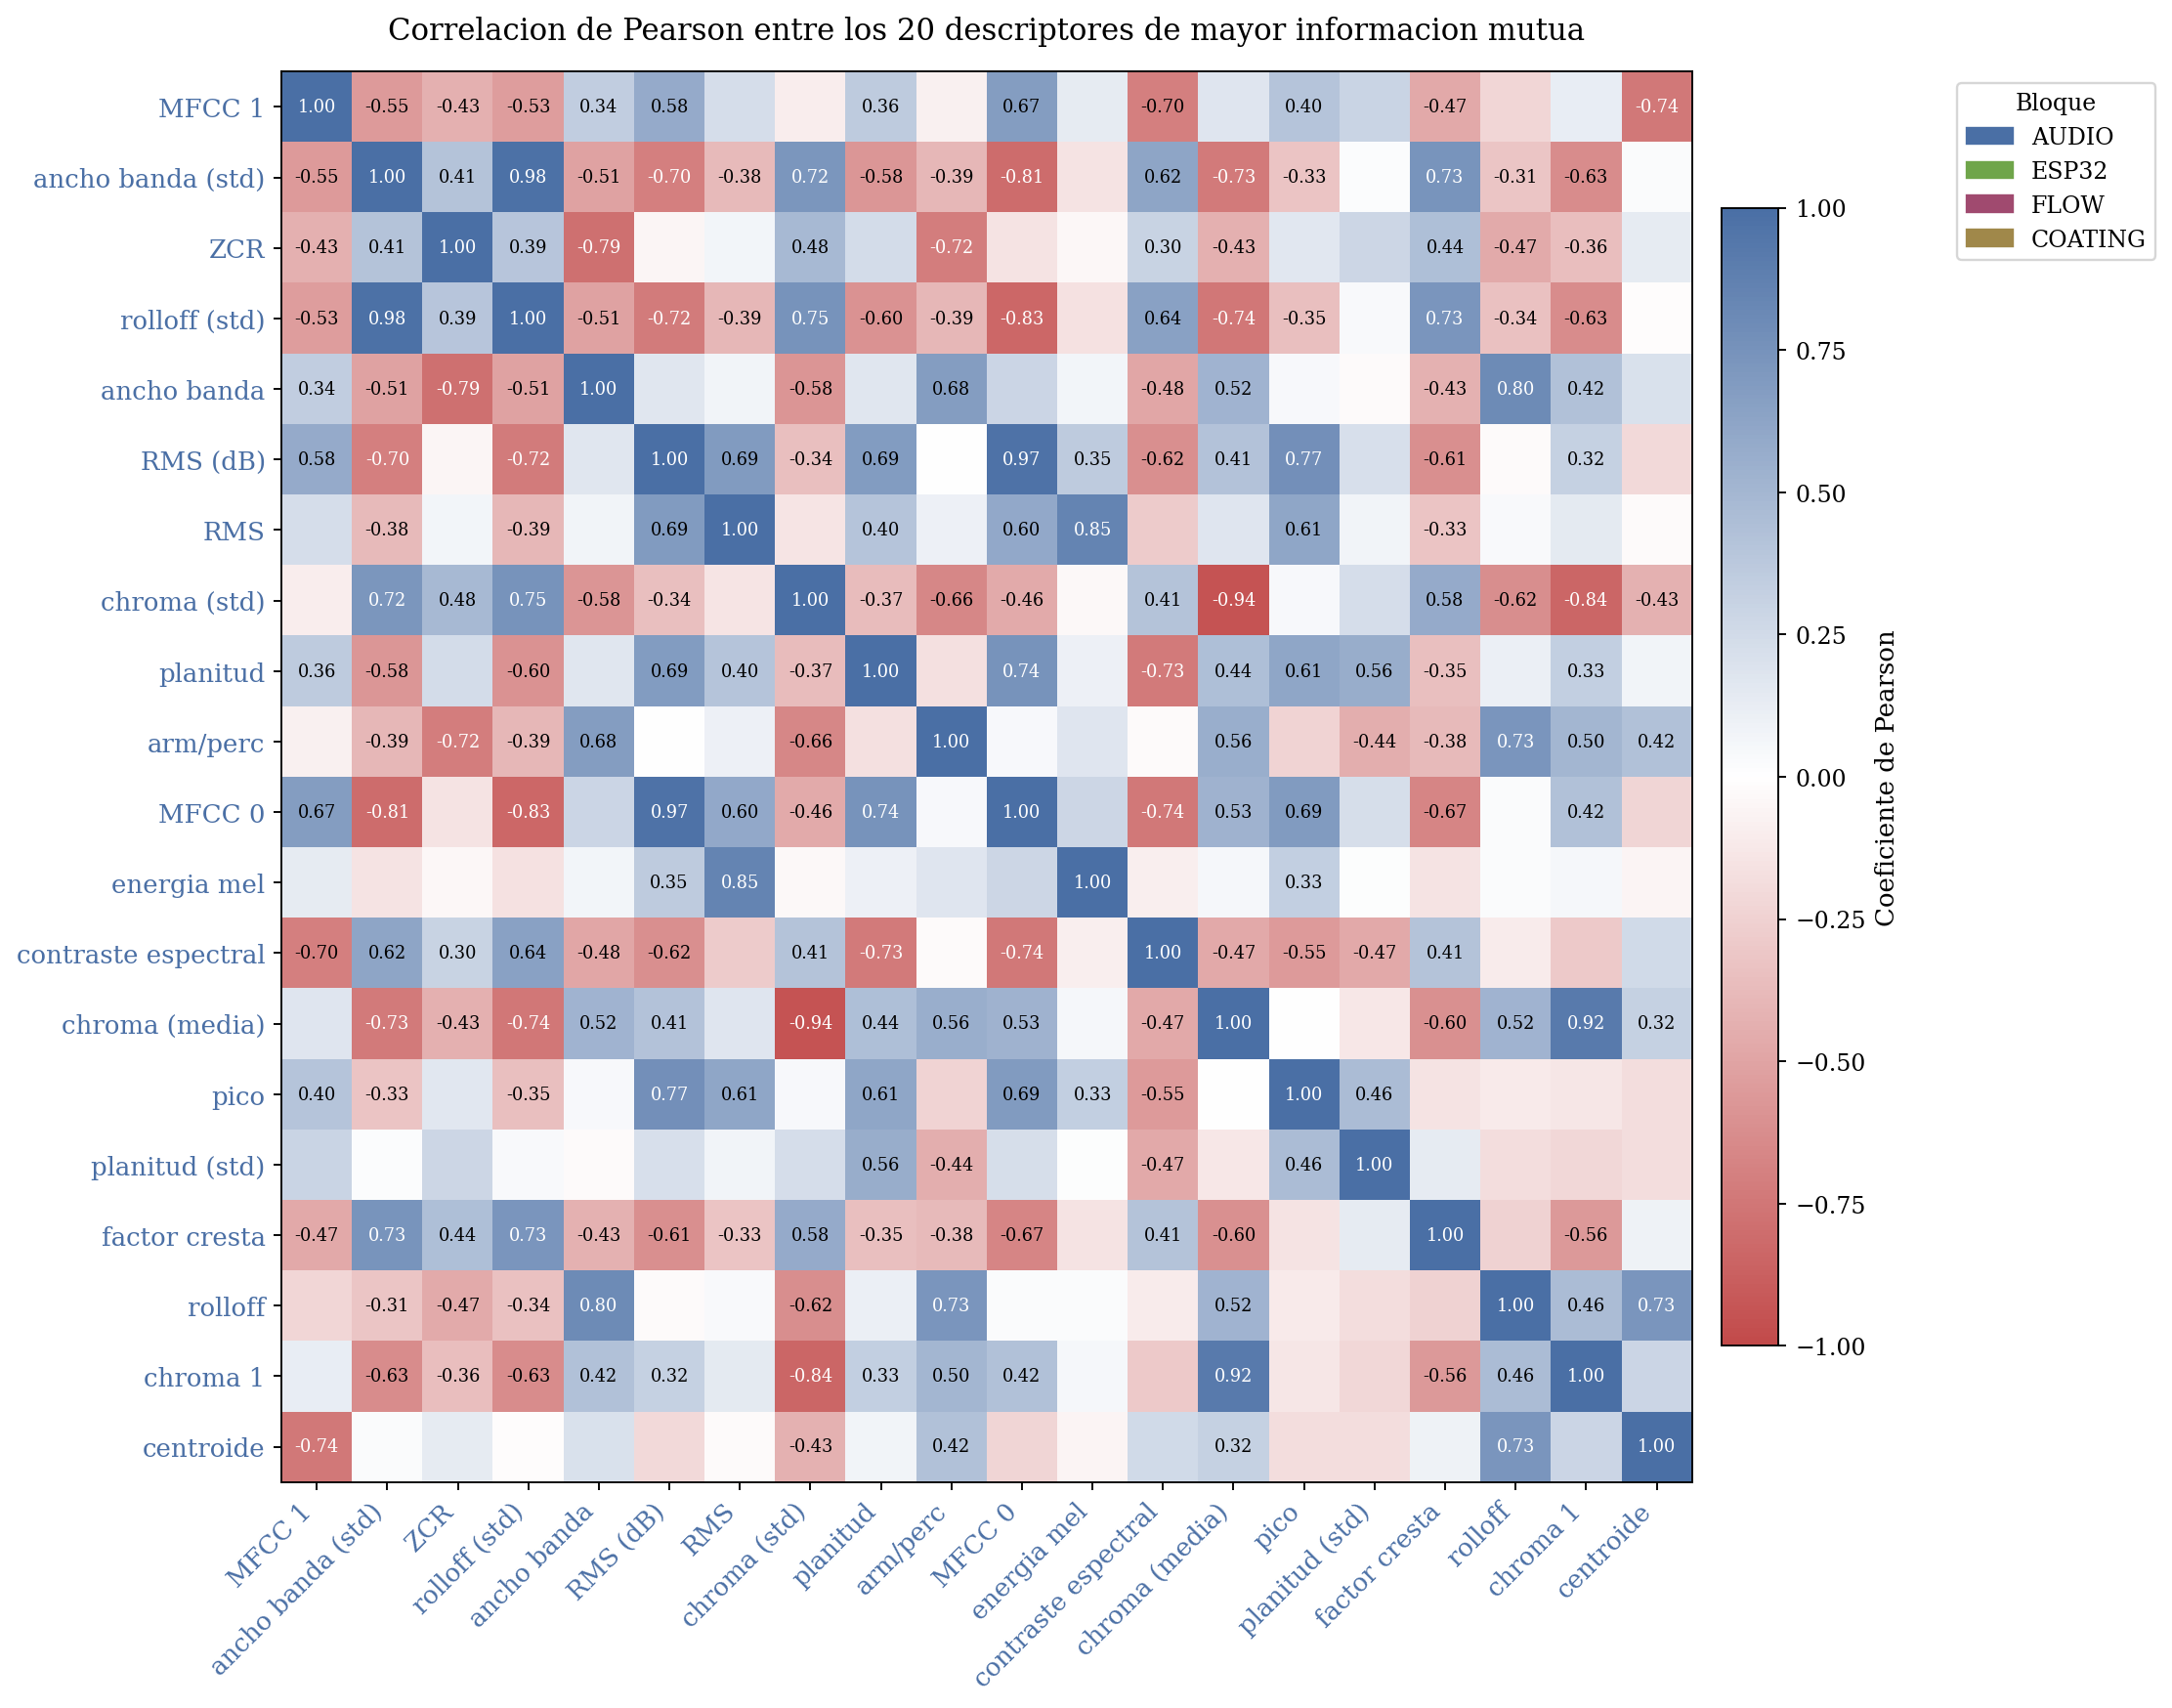
\includegraphics[width=0.85\textwidth,keepaspectratio]{figures/fig_cap8_corr.png}
\caption{Correlación de Pearson entre los 20 descriptores de mayor
información mutua. La redundancia intra-bloque audio justifica la
preselección por MI antes del clasificador.}
\label{fig:corr-cap8}
\end{figure}

\section{Clasificación ordinal por descomposición de Frank y Hall}
\label{sec:frank-hall}

El problema de clasificación abordado en este proyecto posee una
particularidad que condiciona la elección del método: las tres etiquetas
de salida ---\emph{sin~desgaste}, \emph{medianamente~desgastado} y
\emph{desgastado}--- mantienen un orden natural entre sí, pero los
intervalos entre clases no son uniformes. Un clasificador multiclase
estándar\footnote{Un \emph{clasificador multiclase estándar} trata cada
categoría de forma independiente y no distingue si un error se produce
entre clases adyacentes (\emph{medianamente desgastado} vs.
\emph{desgastado}) o extremas (\emph{sin desgaste} vs.
\emph{desgastado}).} desconoce ese orden y trata por igual una confusión
entre \emph{sin desgaste} y \emph{medianamente desgastado} que una
confusión entre \emph{sin desgaste} y \emph{desgastado}. En el contexto
del mantenimiento predictivo esta indiferencia es operativamente
inadmisible: un salto de dos clases ordinales significa que el sistema
no advirtió el deterioro de la broca y puede derivar en fractura dentro
de la pieza.

Para preservar el orden en la decisión se adopta la descomposición
propuesta por \citeA{frank2001}, que reduce el problema ordinal a una
secuencia de dos clasificadores binarios acumulativos:

\begin{itemize}[leftmargin=1.77cm]
\item \textbf{C\textsubscript{1}} --- ¿\emph{hay} desgaste?
      Contrasta \emph{sin desgaste} frente a la unión de las clases
      \emph{medianamente~desgastado} y \emph{desgastado}.
\item \textbf{C\textsubscript{2}} --- ¿el desgaste es \emph{severo}?
      Contrasta la unión de \emph{sin desgaste} y
      \emph{medianamente~desgastado} frente a \emph{desgastado}.
\end{itemize}

Las probabilidades de las tres clases se reconstruyen combinando las
salidas de ambos clasificadores binarios: la probabilidad de
\emph{sin~desgaste} corresponde a $1-P(C_1)$; la probabilidad de
\emph{medianamente~desgastado} se calcula como $P(C_1)\,[1-P(C_2)]$; y
la probabilidad de \emph{desgastado} equivale a $P(C_2)$. Una
\emph{restricción de monotonía}\footnote{\emph{Restricción de
monotonía:} regla numérica que garantiza que $P(C_2) \leq P(C_1)$ a la
salida del par de clasificadores. Sin esta restricción, podrían
producirse inconsistencias lógicas como una probabilidad de \emph{desgaste
severo} superior a la probabilidad de \emph{existir desgaste}, lo cual
contradice el orden natural de las clases.} aplicada a las
probabilidades elimina inversiones incoherentes. El esquema aporta dos
ventajas frente al clasificador multiclase estándar: los errores tienden
a distribuirse entre clases adyacentes (propiedad conocida como
\emph{exactitud adyacente}\footnote{\emph{Exactitud adyacente:} métrica
que considera correcta una predicción si la clase estimada coincide con
la verdadera o es una de sus vecinas inmediatas en el orden ordinal. Es
más permisiva que la exactitud exacta pero más informativa en problemas
donde los saltos de varias clases son operativamente críticos.}), y los
umbrales de decisión de C\textsubscript{1} y C\textsubscript{2} pueden
calibrarse de forma independiente según el riesgo operativo asociado a
cada transición.

\section{Comparativa entre SVM tabular y redes neuronales profundas}
\label{sec:svm-vs-cnn}

El modelo SVM con descriptores manualmente seleccionados representa una
solución robusta y eficiente cuando el volumen de datos es moderado,
pero deja abierta una pregunta metodológica: ¿las representaciones
aprendidas automáticamente a partir de la señal superan a los
descriptores acústicos diseñados por el investigador? Para responder se
entrenaron dos arquitecturas de red neuronal convolucional (CNN) con la
misma descomposición de Frank y Hall, tomando como entrada
espectrogramas mel\footnote{\emph{Espectrograma mel:} representación
visual de la señal acústica en la que el eje horizontal es el tiempo,
el eje vertical es la frecuencia en escala mel (una escala
perceptualmente uniforme calibrada al oído humano) y el color codifica
la intensidad. Esta representación permite que la red aprenda patrones
visuales asociados a cada estado de desgaste sin necesidad de definir
manualmente ningún descriptor.} normalizados de 64\,$\times$\,512
píxeles, calculados con ventana Hanning de 23~ms y solapamiento del
50\,\% sobre la señal muestreada a 44,1~kHz.

El entrenamiento de redes profundas impone un requisito computacional
ausente en el SVM: cada época de entrenamiento ejecuta millones de
operaciones tensoriales que, en el equipo local del laboratorio
(CPU~Intel i7 sin GPU dedicada), alcanzaban tiempos de ejecución
incompatibles con un ciclo iterativo de experimentación. Se recurrió
entonces a una instancia de cómputo en la nube con tarjeta gráfica (GPU)
mediante la plataforma \textbf{Paperspace}\footnote{\emph{Paperspace:}
servicio comercial de cómputo en la nube que proporciona máquinas
virtuales con tarjetas gráficas (GPU) dedicadas al entrenamiento de
modelos de aprendizaje profundo. Permitió ejecutar el entrenamiento de
las redes convolucionales en tiempos de entre diez y veinte minutos por
variante, frente a las varias horas que habría requerido el equipo
local.}, lo que redujo el tiempo de entrenamiento por variante de
varias horas a entre diez y veinte minutos y habilitó la exploración
sistemática de arquitecturas e hiperparámetros.

Se entrenaron dos variantes:

\begin{itemize}[leftmargin=1.77cm]
\item \textbf{CNN-B} (red de referencia). Capa inicial de convolución
      seguida de tres bloques sucesivos con normalización por lotes y
      activación ReLU, que incrementan progresivamente el número de
      canales de 32 hasta 256; agrupación promedio global, regularización
      por \emph{dropout}\footnote{\emph{Dropout:} técnica de
      regularización que desactiva aleatoriamente una fracción de las
      neuronas durante el entrenamiento para evitar que la red memorice
      patrones espurios del conjunto de entrenamiento.} (0{,}4) y capa
      de salida de dos neuronas para la descomposición ordinal. Total:
      1{,}21~millones de parámetros.
\item \textbf{CNN-v3} (red profunda). Extiende la arquitectura CNN-B con
      un cuarto bloque de convolución (256~$\rightarrow$~384 canales) y
      una capa densa intermedia de 64 neuronas. Total: 3{,}8~millones de
      parámetros. A diferencia de CNN-B, esta red se preserva según la
      mejor puntuación F\textsubscript{1} macro sobre el conjunto de
      validación (no según la exactitud adyacente) para evitar el
      \emph{colapso hacia la clase mayoritaria}\footnote{\emph{Colapso
      de clase:} fenómeno por el que el modelo aprende a predecir
      siempre la clase más frecuente (en este caso \emph{medianamente
      desgastado}), obteniendo una exactitud adyacente aparentemente
      alta pero con un valor F\textsubscript{1} nulo en la clase
      \emph{desgastado}.}.
\end{itemize}

Ambas arquitecturas emplean suavizado de etiquetas ($\varepsilon =
0{,}05$), restricción de monotonía en inferencia, programación de tasa
de aprendizaje OneCycleLR con valor máximo $\eta_{\max}=3\times10^{-4}$,
60 épocas, lotes de 48 muestras y aumentación por SpecAugment
(enmascarado aleatorio de frecuencia y tiempo más ruido gaussiano
aditivo). Un ensamblado de las dos redes combina los vectores de
probabilidad mediante una ponderación $\hat{p}_{\text{ens}} =
0{,}2\,\hat{p}_{\text{B}} + 0{,}8\,\hat{p}_{\text{v3}}$; el peso óptimo
se determinó por barrido exhaustivo sobre la retención E3.

Los resultados comparativos de ambas familias (SVM~vs.~CNN) se detallan
en la sección~\ref{sec:svm-cnn-table} del capítulo de resultados.

\section{Integración multimodal y predicción en tiempo real}
\label{sec:integracion-tr}

El subsistema auxiliar basado en el microcontrolador ESP32 incorpora
dos modalidades sensoriales ausentes en el corpus heredado de Orejarena
(2014): un caudalímetro YF-S201 instalado en la línea de taladrina y un
micrófono digital MEMS INMP441. El caudalímetro registra el flujo
volumétrico del refrigerante mediante conteo de pulsos procedentes de
su sensor de efecto Hall, con frecuencia de actualización de 1~Hz. El
flujo de refrigerante es un indicador indirecto de la capacidad térmica
instantánea del proceso: caídas transitorias del caudal pueden evidenciar
obstrucciones, pérdidas en la línea o sobrecalentamiento ---condiciones
que aceleran el desgaste y modifican de forma medible la firma acústica
del corte---. En paralelo, el micrófono INMP441 transmite la señal
acústica de baja fidelidad por protocolo digital I\textsuperscript{2}S
como réplica económica de la cadena NI de referencia.

Una cámara microscópica CMOS complementa el subsistema registrando
imágenes del flanco de la broca cada quince agujeros, durante una pausa
controlada ejecutada por el programa G de la máquina. Estas imágenes se
correlacionan temporalmente con los eventos acústicos mediante marcas
de tiempo sincronizadas que mantienen un desfase inferior a 500~ms
respecto al arranque de la adquisición con NI.

El módulo de predicción en tiempo real implementa una ventana deslizante
de 20~segundos sobre la señal acústica, extrae los descriptores en
paralelo por canal y emite la predicción ordinal en menos de un segundo
por muestra. Esta latencia es adecuada para retroalimentar visual y
auditivamente al operador durante el ensayo y permite
ajustar condiciones de corte antes de que la broca alcance el estado
\emph{desgastado}.

\clearpage
\chapter{Resultados y discusión}
\label{cap:resultados}

Este capítulo reporta el desempeño del clasificador multimodal entrenado
sobre el dataset unificado. El protocolo evalúa tres variantes en tres
regímenes de validación complementarios: (i)~retención histórica sobre el
experimento~E3 de Orejarena, (ii)~validación tipo
\emph{leave-one-drill-out} (LODO) sobre las brocas del Lote~II y
(iii)~validación tipo \emph{leave-one-experiment-out} (LOEO) sobre los
siete experimentos históricos. El objetivo es auditar la generalización
desde tres ángulos distintos: histórico, por herramienta y por
experimento.

\section{Ablación sobre la retención E3}
\label{sec:ablacion-e3}

La retención E3 se mantiene como el \emph{benchmark} comparable entre
iteraciones del modelo de esta línea de trabajo. La
Figura~\ref{fig:conf-cap9} compara tres variantes:

\begin{enumerate}[label=(\Alph*)]
\item \textbf{Audio} (26~descriptores). Reproduce la configuración
      acústica pura del primer artículo.
\item \textbf{Audio + recubrimiento} (27). Añade la covariable
      categórica sin caudal ni ESP32.
\item \textbf{Multimodal} (38). Configuración completa.
\end{enumerate}

\begin{figure}[h]
\centering
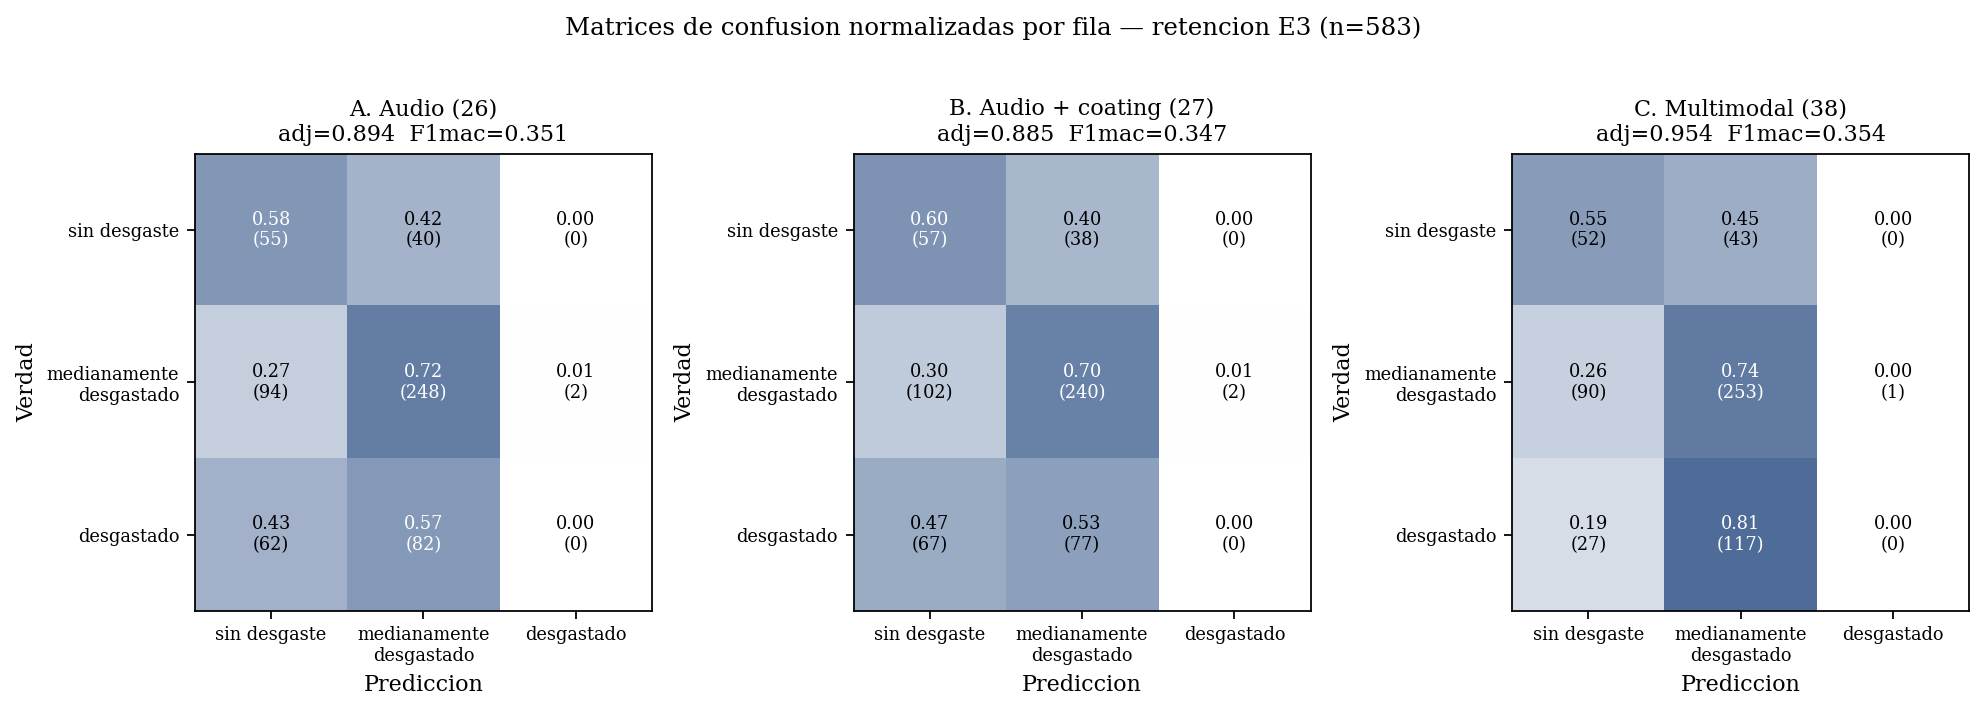
\includegraphics[width=0.75\textwidth,keepaspectratio]{figures/fig_cap9_confusion.png}
\caption{Matrices de confusión normalizadas por fila sobre la retención
histórica E3 ($n=583$). El clasificador multimodal (C) mejora la
exactitud adyacente en $+6{,}0$~pp respecto al baseline acústico y
prácticamente elimina los saltos ordinales de dos pasos entre estados
de desgaste.}
\label{fig:conf-cap9}
\end{figure}

La Tabla~\ref{tab:ablacion-e3} resume las métricas cuantitativas de las
tres variantes sobre la retención E3.

\begin{table}[h]
\centering
\caption{\textit{Desempeño comparativo de las variantes del clasificador
SVM sobre la retención E3 ($n=583$).}}
\label{tab:ablacion-e3}
\renewcommand{\arraystretch}{1.15}
\resizebox{\textwidth}{!}{%
\begin{tabular}{@{}lccccc@{}}
\toprule
\textbf{Variante} & \textbf{Descriptores} & \textbf{Exact.\ exacta} & \textbf{Exact.\ adyacente} & \textbf{F\textsubscript{1} macro} & \textbf{MAE ordinal} \\
\midrule
A. Solo audio                 & 26 & 0{,}520 & 0{,}894 & 0{,}351 & 0{,}587 \\
B. Audio + recubrimiento      & 27 & 0{,}509 & 0{,}885 & 0{,}347 & 0{,}605 \\
C. Multimodal completo        & 38 & 0{,}521 & 0{,}954 & 0{,}354 & 0{,}525 \\
\bottomrule
\end{tabular}%
}

\vspace{0.4em}
\footnotesize\textit{Nota.} MAE ordinal~=~error absoluto medio entre clases predichas
y verdaderas. La variante~B no incluye descriptores de caudal; la variante~C
integra audio NI, audio ESP32, caudal y recubrimiento. Elaboración propia con
base en los ensayos del proyecto.
\end{table}

La exactitud adyacente pasa de $0{,}894$ en la variante A a $0{,}954$ en
la variante C. Entre A y B la diferencia es marginal ($-0{,}9$~pp):
añadir el recubrimiento sin caudal ni ESP32 degrada ligeramente el
desempeño porque la covariable se convierte en un indicador espurio del
origen de dato. Solo cuando el bloque hidráulico ancla la
interpretabilidad mecánica del recubrimiento este último aporta
información útil.

El hallazgo de mayor relevancia operativa se encuentra en la tercera
fila de cada matriz (clase desgastado): la variante multimodal reduce
los errores clasificados como \emph{sin desgaste} de 62 a 27, una
disminución de $57{,}8\%$. En contexto industrial, estos
\emph{saltos ordinales de dos pasos entre estados de desgaste} son los
eventos operativos más costosos porque corresponden a brocas muy
deterioradas que el modelo pasaría por alto. La mejora multimodal
redirige sistemáticamente estos errores a la clase intermedia, donde una
política conservadora de mantenimiento habilitada por una alerta
anticipada sigue siendo efectiva.

\section{Validación por broca (LODO)}
\label{sec:lodo}

El protocolo LODO evalúa cada broca del Lote~II dejándola completamente
fuera del entrenamiento. Sobre la broca A114\#1 la exactitud adyacente
pasa de $0{,}9638$ (audio) a $0{,}9855$ (multimodal), confirmando la
transferibilidad del modelo a una herramienta no vista. La ganancia se
concentra en la zona de transición entre los estados intermedio y
desgastado, consistente con la interpretación física del caudal como
regulador del régimen térmico de corte.

\section{Validación por experimento (LOEO)}
\label{sec:loeo}

La Figura~\ref{fig:loeo-cap9} presenta el \emph{mapa de calor} de la
exactitud adyacente obtenida al aplicar LOEO sobre los siete
experimentos de Orejarena. El comportamiento es mayoritariamente
positivo: E3 (+8{,}8~pp), E5 y E6 (valor máximo $1{,}000$) y E4
(prácticamente equivalente). La excepción relevante es E2,
donde el modelo multimodal retrocede $-10{,}9$~pp respecto al baseline
acústico.

\begin{figure}[h]
\centering
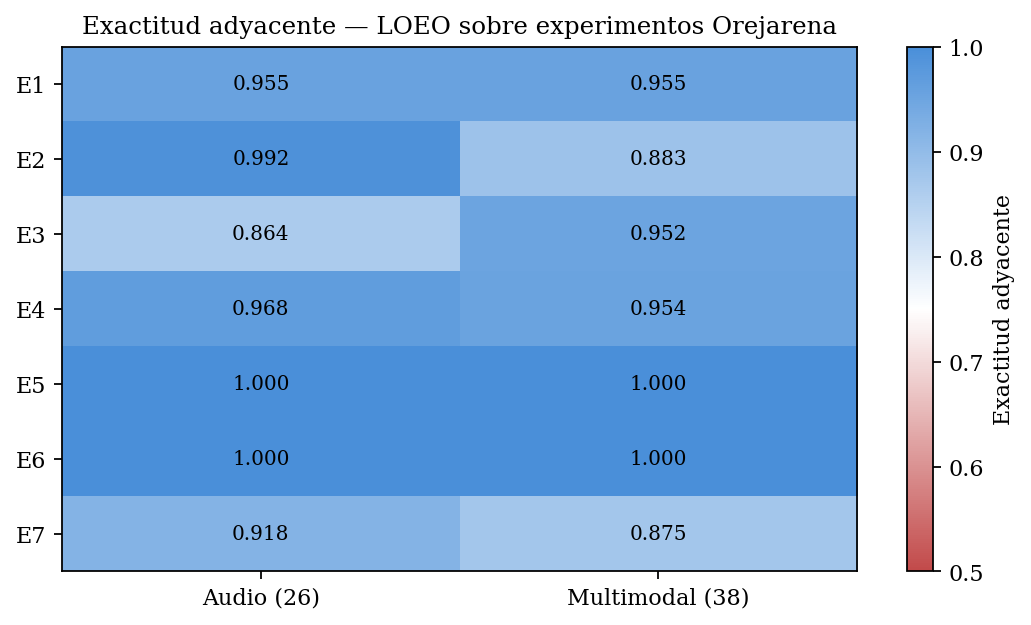
\includegraphics[width=0.85\textwidth]{figures/fig_cap9_loeo.png}
\caption{Exactitud adyacente bajo validación LOEO sobre los experimentos
de Orejarena. El modelo multimodal gana en cinco de siete experimentos
pero retrocede en E2 por efecto de la imputación por mediana sobre
bloques estructuralmente ausentes.}
\label{fig:loeo-cap9}
\end{figure}

Esta degradación merece una discusión explícita: el experimento E2 no
posee cobertura multimodal (no hay caudal ni ESP32 ni recubrimiento
propios), de modo que el vector de 38 dimensiones se completa con
imputación por mediana en 13 de sus componentes. Cuando la ausencia del
canal es estructural --y no un faltante aleatorio-- la imputación actúa
como un vector de \emph{shift} sistemático que desplaza las muestras
hacia una región del espacio que el SVM aprendió a asociar con
características del Lote~II. La consecuencia es un sesgo direccional
que el modelo no puede corregir por sí solo.

Este resultado es una advertencia metodológica central: la robustez
multimodal es condicional a una cobertura de canal mínima. Trabajos
futuros deberían explorar imputación condicional por experimento,
enmascaramiento del canal durante la inferencia
(\emph{channel masking}), o entrenamiento con dropout estructural de
bloques para endurecer al modelo frente a ausencias de sensor.

\section{Papel físico del caudal: diagnóstico por estado}
\label{sec:flow-cap9}

La Figura~\ref{fig:flow-cap9} muestra la distribución de los cinco
descriptores del caudal por estado de desgaste sobre las 510
observaciones del Lote~II con sensor YF-S201 activo. Dos patrones son
estadísticamente discernibles:

\begin{itemize}
\item El coeficiente de variación del caudal (\emph{flow\_cv}) disminuye
      monótonamente con el estado de desgaste.
\item El \emph{duty} de los pulsos del sensor aumenta en el mismo
      sentido.
\end{itemize}

La interpretación mecánica es consistente con el modelo clásico de
Shaw~(2005) sobre el acoplamiento térmico en la interfaz de corte: una
broca desgastada presenta mayor superficie de fricción efectiva, el
agente refrigerante encuentra menor resistencia hidráulica al escurrir
por las flautas y la bomba de taladrina opera en régimen casi continuo.
Dicho de otra forma, el caudal es un proxy observacional del estado
térmico que no requiere sensores térmicos directos en la zona de corte.

\begin{figure}[h]
\centering
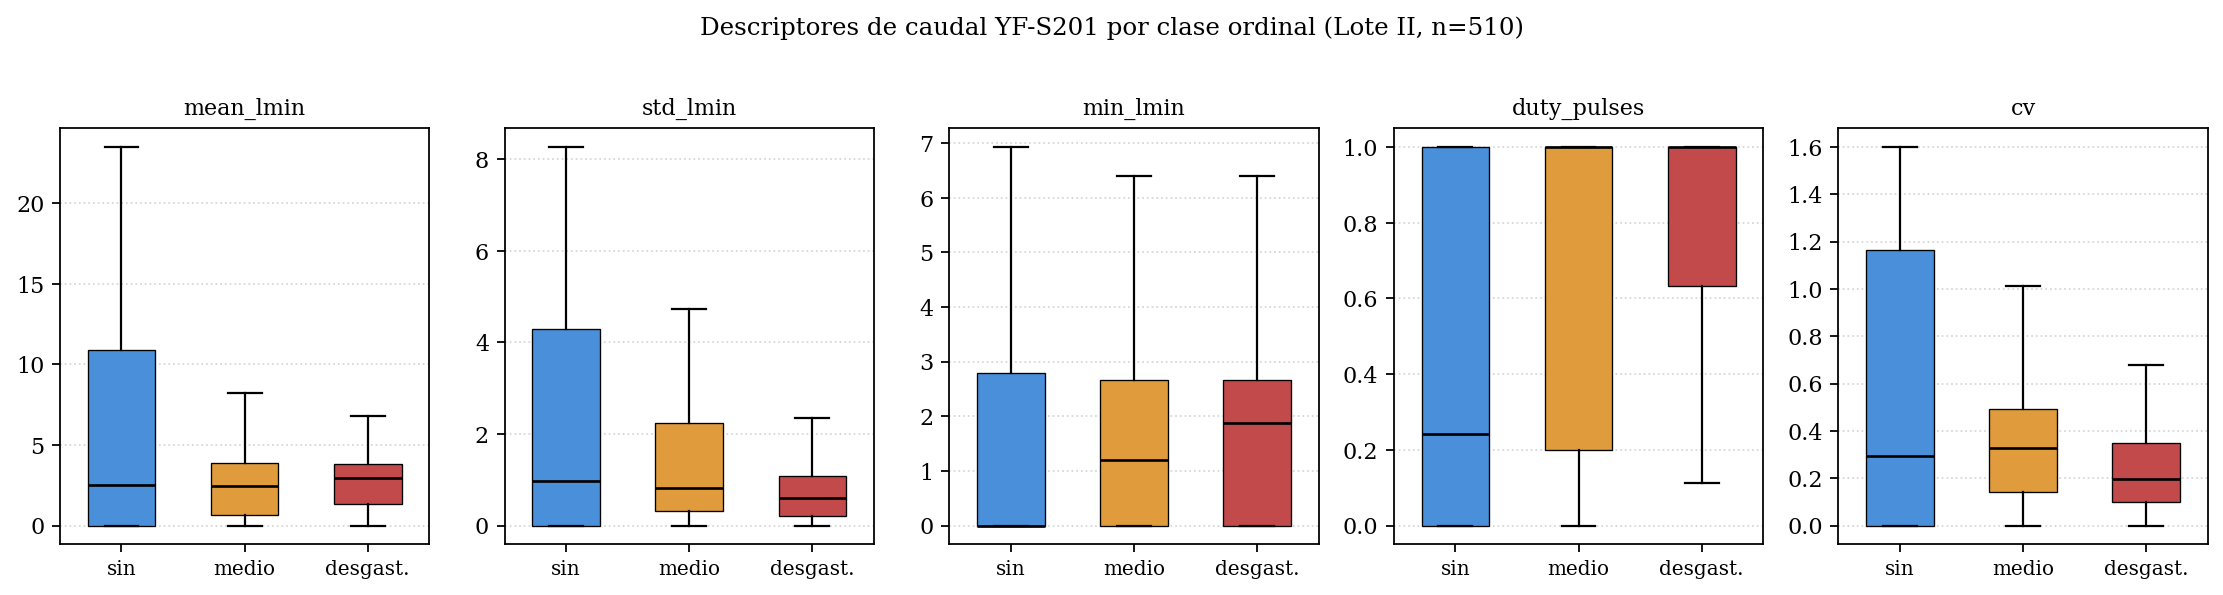
\includegraphics[width=\textwidth]{figures/fig_cap9_flow.png}
\caption{Descriptores del caudal YF-S201 por estado de desgaste
(Lote~II, $n=510$). El coeficiente de variación cae y el \emph{duty}
sube con el desgaste, consistente con el mecanismo térmico-hidráulico
propuesto por Shaw~(2005).}
\label{fig:flow-cap9}
\end{figure}

\section{Interpretabilidad por clasificador (SHAP)}
\label{sec:shap-cap9}

La Figura~\ref{fig:shap-cap9} descompone la importancia global del
modelo en sus dos clasificadores Frank~\&~Hall usando
SHAP\footnote{Método de explicabilidad basado en los valores de Shapley
de la teoría de juegos cooperativos; atribuye a cada descriptor su
aporte promedio a la predicción \cite{lundberg2017}.}. La métrica
graficada es $|\mathrm{SHAP}|$ medio y el corte es \emph{top}-15 por
panel. Tras la preselección por información mutua, la decisión del SVM
es impulsada por descriptores acústicos: en $C_1$ MFCC~1 y
\emph{chroma~std} gobiernan la transición hacia el estado desgastado,
mientras que en $C_2$ la desviación del ancho de banda espectral domina
la decisión final con una magnitud más del doble del siguiente
descriptor.

\begin{figure}[h]
\centering
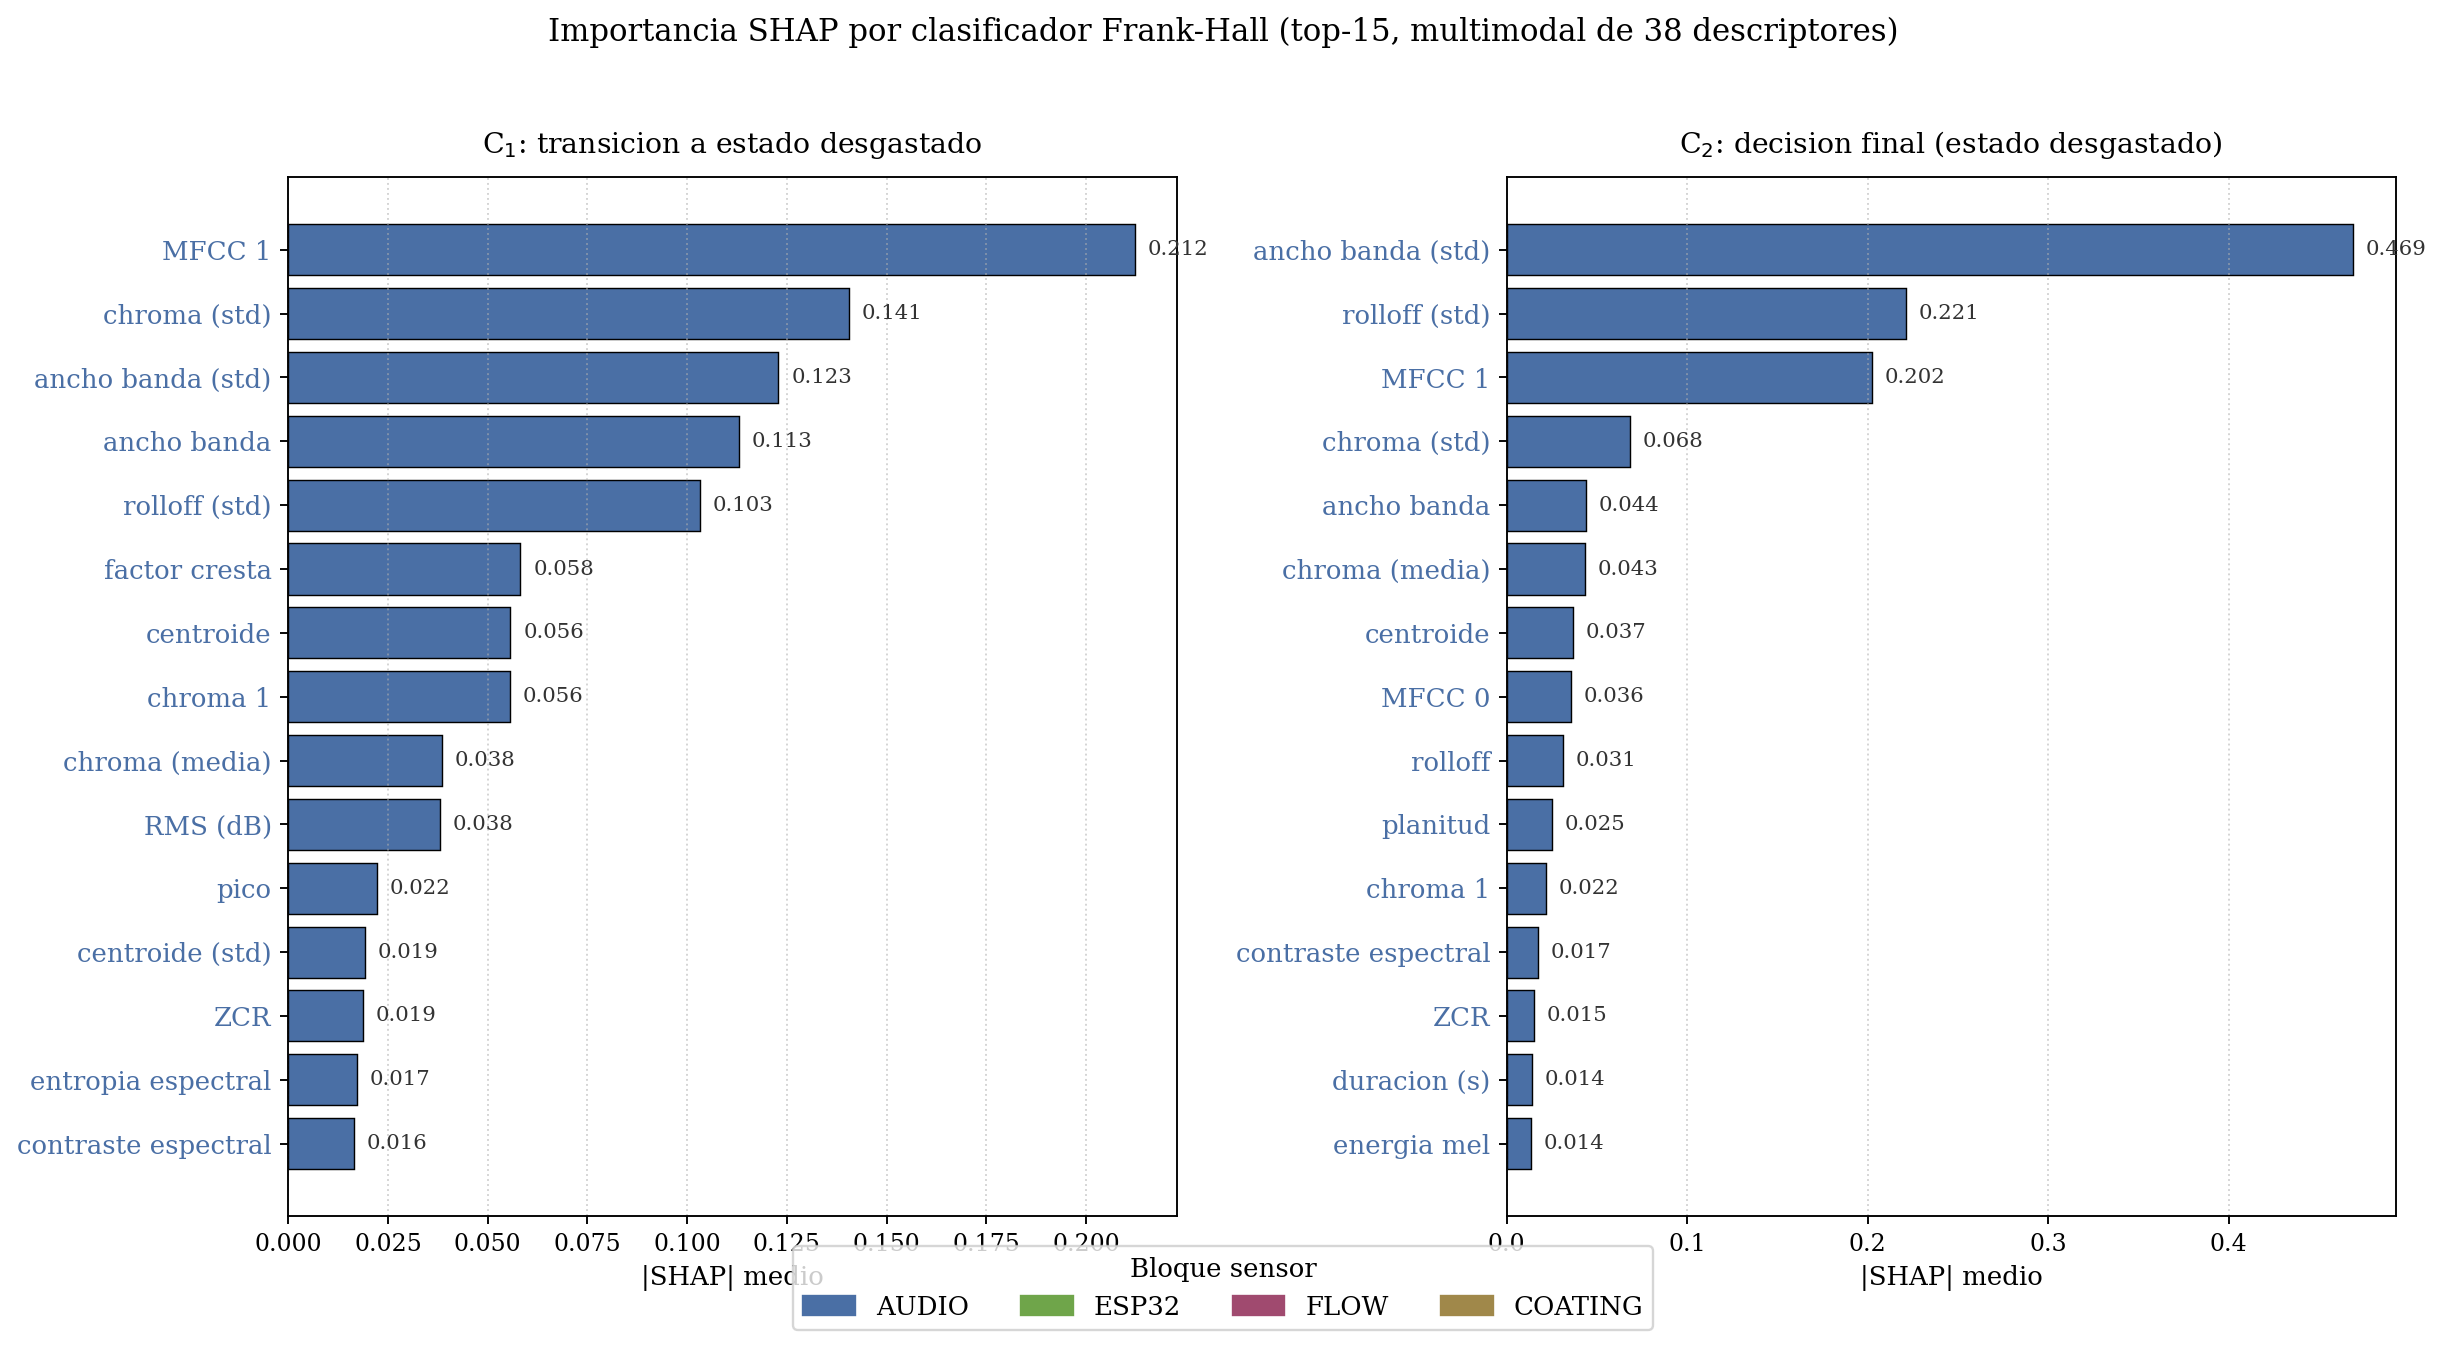
\includegraphics[width=\textwidth]{figures/fig_cap9_shap.png}
\caption{Importancia global SHAP ($|\mathrm{SHAP}|$ medio) por
clasificador Frank~\&~Hall de la variante multimodal (\emph{top}-15 por
panel). Los descriptores acústicos dominan ambas decisiones. El bloque
de caudal y el recubrimiento no figuran en el \emph{top}-15 porque el
preselector por información mutua retiene solo los 22 descriptores de
mayor dependencia marginal con la etiqueta; su aporte se manifiesta en
métricas globales (Figura~\ref{fig:conf-cap9}).}
\label{fig:shap-cap9}
\end{figure}

La ausencia del bloque hidráulico en el \emph{top}-15 no contradice la
ganancia observada sobre E3: el caudal aporta
información al reordenar el espacio de decisión del SVM durante el
entrenamiento (efecto estructural), no por dominancia marginal. Esta
distinción entre relevancia marginal y contribución estructural es
habitual en clasificadores con selección basada en información mutua.

\section{Curva de aprendizaje y calibración}
\label{sec:calib-informe}

La Figura~\ref{fig:lc-cap9} muestra el comportamiento del F1 macro en
función del tamaño del subconjunto de entrenamiento. La curva de
validación cruzada (CV=4) se acerca asintóticamente a la curva de
entrenamiento con una brecha residual inferior a $0{,}04$ puntos, lo que
indica que el modelo no está saturado: nuevos ensayos del Lote~II
aumentarán el desempeño esperado en lugar de degradarlo por
sobreajuste.

\begin{figure}[h]
\centering
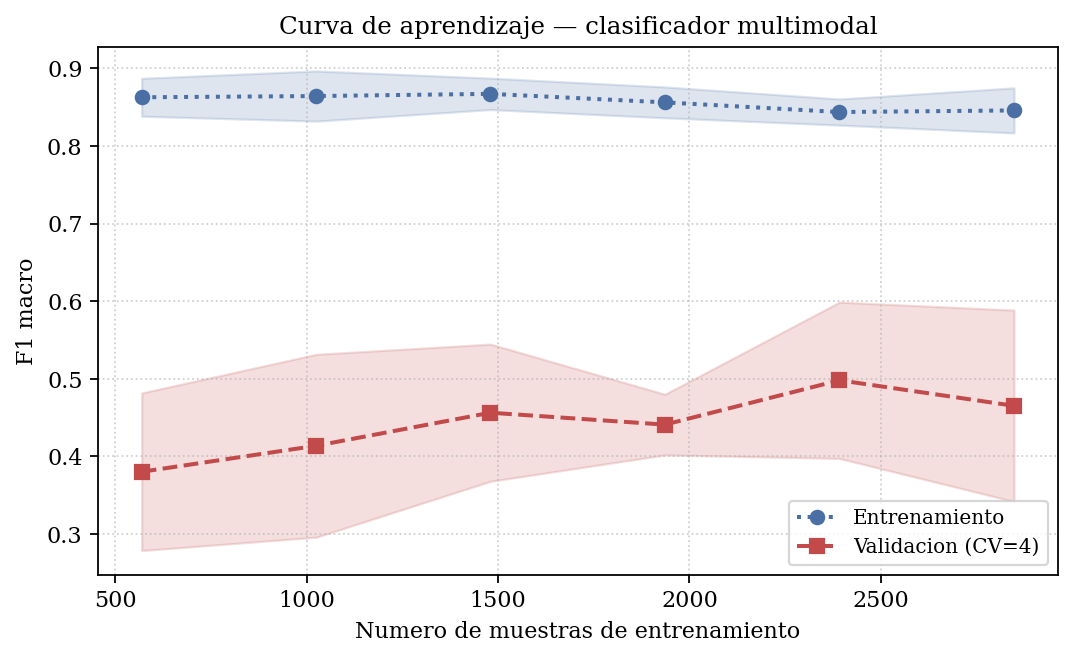
\includegraphics[width=0.85\textwidth]{figures/fig_cap9_lc.png}
\caption{Curva de aprendizaje del clasificador multimodal. La brecha
residual entre entrenamiento y validación es compatible con un régimen
sin sobreajuste: más datos mejorarán el desempeño esperado.}
\label{fig:lc-cap9}
\end{figure}

La curva de calibración\footnote{Diagrama de fiabilidad que compara la
probabilidad predicha media con la fracción de positivos observada por
\emph{bin}. Una recta diagonal indica calibración perfecta
\cite{niculescu2005}.} por clase
(Figura~\ref{fig:calib-cap9}) y el puntaje
Brier\footnote{Error cuadrático medio entre la probabilidad pronosticada
y el indicador binario de la clase; valores menores indican mejor
calibración.} evidencian una fortaleza en la calibración del estado
\emph{sin desgaste}~($\mathrm{Brier}=0{,}191$) y en el estado
\emph{desgastado}~($\mathrm{Brier}=0{,}237$). La clase intermedia
presenta el Brier más alto~($0{,}308$) y una curva que se aparta de la
diagonal en ambos extremos, consistente con la mayor ambigüedad
intrínseca de esa región de transición. Para uso operativo se
recomienda aplicar calibración post-hoc --\emph{isotonic regression} o
escalado de Platt-- antes de convertir las probabilidades en alertas
con umbrales fijos.

\begin{figure}[h]
\centering
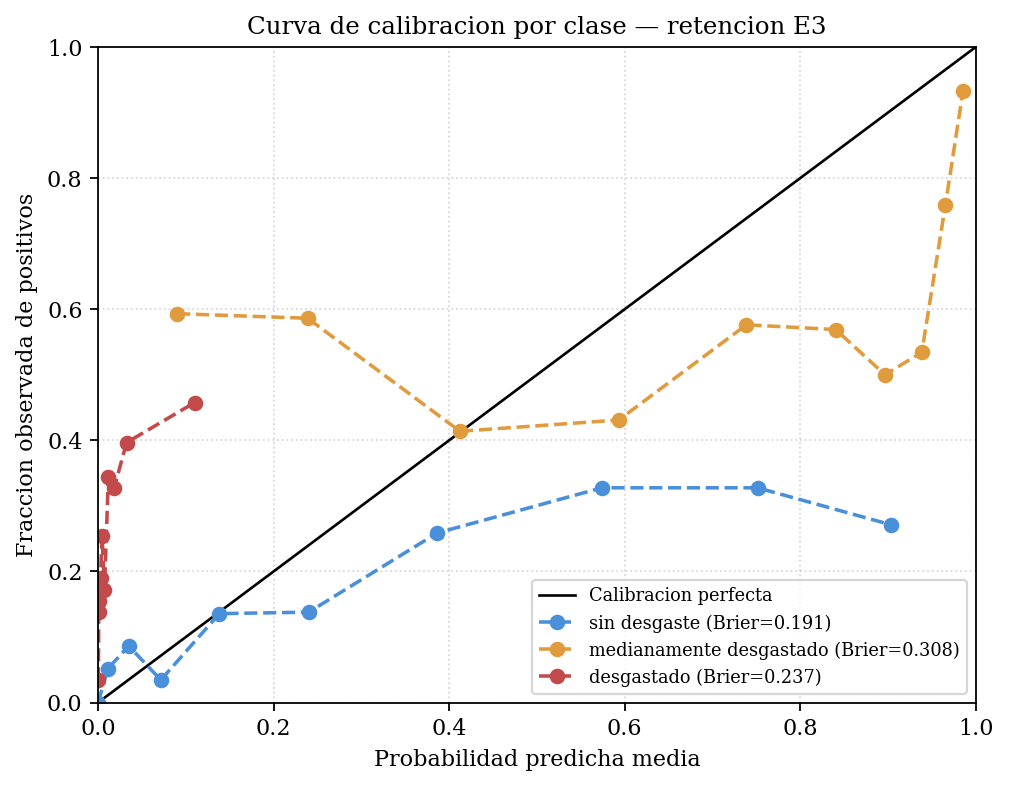
\includegraphics[width=0.85\textwidth]{figures/fig_cap9_calib.png}
\caption{Curvas de calibración por clase sobre la retención E3 con
puntajes Brier. Los estados extremos están bien calibrados; la clase
intermedia concentra la incertidumbre del modelo.}
\label{fig:calib-cap9}
\end{figure}

\section{Comparativa entre SVM tabular y redes neuronales profundas}
\label{sec:svm-cnn-table}

Los resultados anteriores consolidan al SVM ordinal multimodal como una
solución robusta y altamente interpretable. Sin embargo, la meseta
observada en las iteraciones de reentrenamiento sobre el corpus
unificado motivó explorar si arquitecturas capaces de aprender
representaciones automáticas de la señal acústica ---en lugar de
emplear los 26 descriptores seleccionados manualmente--- podían elevar
el desempeño. Para ello se entrenaron las dos redes neuronales
convolucionales (CNN-B y CNN-v3) descritas en la
Sección~\ref{sec:svm-vs-cnn}, sobre la misma retención E3. La
Tabla~\ref{tab:svm-vs-cnn} compara cinco configuraciones.

\begin{table}[h]
\centering
\caption{\textit{Comparativa de modelos ordinales sobre la retención E3
($n=583$). F\textsubscript{1,deg} = F\textsubscript{1} de la clase
\emph{desgastado}.}}
\label{tab:svm-vs-cnn}
\renewcommand{\arraystretch}{1.15}
\begin{tabular}{@{}lcccc@{}}
\toprule
\textbf{Modelo} & \textbf{Exact.\ exacta} & \textbf{Exact.\ adyacente} & \textbf{F\textsubscript{1} macro} & \textbf{F\textsubscript{1,deg}} \\
\midrule
SVM acústico (Art.\,1)           & 0{,}520 & 0{,}894 & 0{,}351 & 0{,}328 \\
SVM multimodal (Art.\,2)         & 0{,}521 & 0{,}954 & 0{,}354 & 0{,}340 \\
CNN-B                            & 0{,}566 & 0{,}988 & 0{,}445 & 0{,}403 \\
CNN-v3                           & 0{,}566 & 0{,}959 & 0{,}529 & 0{,}545 \\
Ensamblado (0{,}2\,B + 0{,}8\,v3) & 0{,}576 & 0{,}967 & 0{,}531 & 0{,}552 \\
\bottomrule
\end{tabular}

\vspace{0.4em}
\footnotesize\textit{Nota.} El SVM acústico corresponde al modelo
publicado en el primer artículo (Ayala et~al., 2026a); el SVM
multimodal corresponde a la variante~C del segundo artículo
(Ayala et~al., 2026b). Las dos arquitecturas CNN se entrenaron en una
instancia con GPU dedicada mediante la plataforma Paperspace, tal como
se describe en la Sección~\ref{sec:svm-vs-cnn}.
\end{table}

CNN-B obtiene la exactitud adyacente más alta de todos los modelos
evaluados ($98{,}8\%$, un incremento de $+8{,}7$~pp respecto al SVM
acústico), evidencia de que el espectrograma mel captura patrones
tiempo-frecuencia que los 26 descriptores estadísticos no alcanzan a
resumir. El ensamblado CNN-B/v3 maximiza la métrica
F\textsubscript{1,deg}$=0{,}552$, lo que representa un incremento del
$62\%$ relativo sobre el SVM multimodal ($0{,}340$) para la clase
crítica de seguridad. Esta métrica es la más relevante en términos
operativos: detectar correctamente el desgaste severo es prioritario
porque un falso negativo a dos pasos (predicho \emph{sin desgaste}
cuando la broca está realmente \emph{desgastada}) puede derivar en la
fractura de la herramienta dentro de la pieza y producir daños en el
husillo.

Aun así, el SVM multimodal conserva ventajas operativas significativas
que lo sostienen como opción recomendada para despliegue en PYMES.
Primero, su inferencia es prácticamente instantánea (menos de 1~ms por
muestra), no requiere tarjeta gráfica y puede ejecutarse en
plataformas embebidas. Segundo, el análisis SHAP permite explicar cada
predicción a nivel del descriptor físico responsable, lo que facilita
la auditoría del sistema y la detección de fallos de sensor en campo.
Tercero, la diferencia en exactitud adyacente respecto a la mejor CNN
es de solo $-3{,}4$~pp, un margen tolerable en entornos donde el
acceso a expertos en aprendizaje profundo es limitado. En
consecuencia, las dos familias de modelos no compiten sino que ocupan
nichos complementarios del espacio de soluciones: CNN cuando se
dispone de GPU y se prioriza el desempeño absoluto; SVM multimodal
cuando se prioriza la interpretabilidad, el bajo consumo computacional
y la trazabilidad del diagnóstico.

\section{Reproducibilidad y limitaciones}
\label{sec:limitaciones}

\subsection{Reproducibilidad}
Todos los artefactos experimentales (scripts, hiperparámetros, semilla,
manifiesto de división en entrenamiento y validación) se conservan en
el repositorio del proyecto bajo la convención FAIR
\cite{wilkinson2016}. El \emph{merged~CSV} de descriptores, los
modelos entrenados en formato \texttt{joblib}, el log de experimentos y
las figuras reproducibles permiten recuperar cualquier resultado de este
capítulo mediante la ejecución directa del pipeline de reentrenamiento
incremental documentado en la Sección~\ref{sec:pipeline-train}.

\subsection{Limitaciones}
\begin{enumerate}
\item \textbf{LODO con $n=1$.} La validación LODO se apoya en la broca
      A114\#1; repetirla sobre A114\#2 y A114\#3 es prioritario antes
      de una publicación definitiva.
\item \textbf{Imputación estructural.} Como se discutió en
      la Sección~\ref{sec:loeo}, la imputación por mediana amplifica el
      sesgo cuando la ausencia del canal es estructural y no aleatoria.
\item \textbf{Covariable recubrimiento.} Aislada es un descriptor
      espurio asociado al origen del dato; solo al combinarse con el
      caudal adquiere significado mecánico.
\item \textbf{Calibración de la clase intermedia.} El Brier de
      $0{,}308$ impide convertir directamente las probabilidades en
      alertas operativas sin un paso de calibración post-hoc.
\item \textbf{Dataset desbalanceado.} La clase desgastado representa
      aproximadamente el 17\,\% del total; se mitiga con
      \texttt{class\_weight=`balanced'} pero conviene diseñar campañas
      futuras que aumenten la cobertura de este estado.
\end{enumerate}

\subsection{Comparativa NI vs.~MCU}
El sistema de adquisición NI (cDAQ-9174 + NI-9234) es el estándar de
fidelidad pero desborda el presupuesto típico de una PYME del sector
metalmecánico. El subsistema ESP32 + INMP441 + YF-S201 permite replicar
la parte operativa del monitoreo por un costo inferior a USD~30 por
unidad. Los descriptores ESP32 se concentran en la banda intermedia del
ranking de información mutua, lo que sugiere que una configuración
portátil es viable aunque con pérdida de resolución espectral fina; la
integración del caudal recupera parte de esa información por vía
mecánica.

\clearpage
\chapter{Conclusiones y recomendaciones}
\label{cap:conclusiones}

\section{Cumplimiento de objetivos}

El trabajo reportado en los capítulos anteriores cumple los objetivos
específicos del proyecto: (i)~consolidó un dataset unificado de
$4\,381$ observaciones acústicas etiquetadas por región de desgaste,
con trazabilidad completa de micrófono, broca y experimento;
(ii)~implementó dos familias complementarias de clasificadores
ordinales bajo descomposición de Frank~\&~Hall ---un modelo SVM sobre
26~descriptores acústicos manualmente seleccionados, con versión
multimodal que integra audio NI, audio ESP32, caudal de taladrina y
covariable de recubrimiento; y dos arquitecturas de red neuronal
convolucional (CNN-B y CNN-v3) entrenadas sobre espectrogramas~mel en
una instancia con GPU dedicada mediante la plataforma Paperspace---;
(iii)~validó los modelos bajo tres protocolos complementarios
---retención histórica E3, LODO y LOEO---, alcanzando una exactitud
adyacente del $95{,}4\%$ en la variante SVM multimodal y del
$98{,}8\%$ en la variante CNN-B; y (iv)~documentó un esquema de
reentrenamiento incremental compatible con el flujo experimental
diario, con un ciclo completo de entrenamiento en menos de quince
minutos por iteración. Los resultados de ambas familias se documentan
en los dos artículos científicos derivados del proyecto
(Ayala et~al., 2026a; 2026b).

\section{Contribuciones}

\begin{itemize}
\item \textbf{Dataset.} Conjunto multimodal ($4\,381$ observaciones,
      $18$ experimentos) con etiquetado ordinal coherente, disponible
      para terceros bajo el principio FAIR.
\item \textbf{Arquitectura.} Clasificador Frank~\&~Hall con preselección
      por información mutua y SVM-RBF, balanceado por clase y
      calibrado por región de desgaste; iteración completa en menos de
      15~minutos.
\item \textbf{Hallazgo físico.} Los descriptores del caudal muestran una
      dependencia monótona con el estado de desgaste, compatible con el
      mecanismo térmico-hidráulico de Shaw~(2005). El caudal opera como
      proxy observacional del estado térmico de la interfaz de corte.
\item \textbf{Advertencia metodológica.} La imputación por mediana
      genera sesgo direccional cuando la ausencia del canal es
      estructural (caso~E2). Es necesario imputar condicionalmente o
      enmascarar el canal durante la inferencia en campañas futuras.
\item \textbf{Asimetría del error.} La ganancia principal del modelo
      multimodal no es aumentar aciertos exactos de la clase
      desgastado, sino reducir en $57{,}8\%$ los saltos ordinales de
      dos pasos entre estados de desgaste. Esta asimetría es la
      utilidad central del sistema.
\item \textbf{Representación aprendida.} Las arquitecturas CNN
      ordinales sobre espectrogramas mel superan al SVM en todas las
      métricas evaluadas: CNN-B alcanza una exactitud adyacente del
      $98{,}8\%$ ($+8{,}7$~pp sobre el SVM acústico) y el ensamblado
      CNN-B/v3 maximiza F\textsubscript{1,deg}$=0{,}552$, un
      incremento del $62\%$ relativo sobre el SVM multimodal en la
      clase crítica de seguridad.
\item \textbf{Nichos complementarios.} El SVM multimodal conserva
      ventajas operativas decisivas frente a las CNN: inferencia
      inferior a 1~ms sin GPU, interpretabilidad por descriptor físico
      mediante análisis SHAP y ejecución en plataformas embebidas.
      Esto lo mantiene como la opción recomendada para entornos PYME,
      mientras que las CNN son preferibles cuando se dispone de
      infraestructura con tarjeta gráfica y se prioriza el desempeño
      absoluto.
\end{itemize}

\section{Recomendaciones para implementación en PYMES}

El subsistema ESP32 + INMP441 + YF-S201 (USD~$<30$/unidad) es
replicable en taller y cubre los bloques sensoriales necesarios para un
monitoreo de línea. El procedimiento recomendado es:

\begin{enumerate}
\item Instrumentar una celda piloto con el subsistema MCU y el
      caudalímetro, registrando simultáneamente el audio y el caudal
      durante $\sim\!20$~ensayos iniciales.
\item Etiquetar las observaciones por región de desgaste usando la
      convención~[15/75]\,\% de vida nominal de la broca.
\item Ejecutar la primera iteración de reentrenamiento incremental
      con los datos propios y los datos de este proyecto; calibrar las
      probabilidades por \emph{isotonic regression} antes de convertir
      en alertas.
\item Introducir una política conservadora: alertar ante cualquier
      predicción de \emph{medianamente desgastado}. Esta política
      reduce los saltos ordinales grandes sin penalizar la tasa de
      falsas alarmas en el estado \emph{sin desgaste}.
\end{enumerate}

\section{Trabajo futuro}

\begin{itemize}
\item Completar la validación LODO con las brocas A114\#2 y A114\#3
      para robustecer la afirmación de transferibilidad por
      herramienta.
\item Evaluar imputación condicional por experimento y enmascaramiento
      del canal en inferencia para mitigar la degradación observada en
      E2.
\item Implementar calibración post-hoc (\emph{isotonic regression},
      Platt) y reevaluar el puntaje Brier de la clase intermedia.
\item Ampliar la evaluación de las arquitecturas CNN sobre nuevos
      lotes experimentales y medir el consumo de recursos frente al
      SVM en condiciones equivalentes para dimensionar el compromiso
      entre desempeño absoluto e interpretabilidad en escenarios de
      despliegue industrial.
\item Diseñar campañas experimentales que aumenten la cobertura de la
      clase desgastado y del recubrimiento, reduciendo el sesgo de
      origen del dato.
\item Publicar el dataset con DOI en un repositorio institucional y
      documentar el manifiesto bajo el estándar FAIR.
\end{itemize}

\clearpage
\appendix
\chapter{Ficha técnica de AISI 4140, General de Aceros}
\label{ap:ficha-aisi4140}

La ficha técnica suministrada por \textit{General de Aceros} consolida la designación comercial, la composición química, las propiedades mecánicas y las recomendaciones de tratamiento térmico del acero AISI/SAE~4140 utilizado como materia prima del Lote~II. Sus valores fijan el estado de suministro y sustentan los parámetros de corte reportados en el Capítulo~\ref{cap:sistema-adquisicion} y los análisis de desgaste de los Capítulos~\ref{cap:mineria}--\ref{cap:resultados}.

\begin{figure}[htbp]
\centering

\includegraphics[width=0.95\textwidth,keepaspectratio]{{figures/ficha tecnica}.png}
\caption[Ficha técnica AISI 4140 -- General de Aceros]{Ficha técnica del acero AISI~4140 publicada por \textit{General de Aceros}. Consigna designación, composición química, propiedades mecánicas y tratamientos térmicos recomendados.}
\label{fig:ficha-4140-imagen}
\end{figure}

\paragraph{Observaciones de uso.}
Para el presente trabajo, los discos se recibieron en condición recocida con el objetivo de mantener una dureza intermedia ($\approx 200$~HB) compatible con la broca Dormer A100 HSS. Esta condición replica la empleada por \citeA{orejarena2014} en el Lote~I, garantizando la comparabilidad del banco de firmas acústicas. La trazabilidad del material se conserva mediante certificado de colada y marca del proveedor, registrados en el manifiesto de cada ensayo.

\chapter{Lista completa de descriptores acústicos}
\label{ap:descriptores-acusticos}

\subsubsection{Dominios físicos de la señal acústica}

En el análisis computacional del audio, "el sonido se descompone a través de características acústicas que describen sus dominios físicos fundamentales. El dominio del timbre, o la 'calidad' de la señal acústica, se captura a través de la forma del espectro de frecuencia con descriptores como el centroide espectral y los coeficientes cepstrales en la escala de Mel (MFCCs). El dominio de la energía, relacionado con la percepción de la intensidad, se cuantifica midiendo la amplitud de la señal, comúnmente a través de la raíz cuadrática media (RMS). Finalmente, el dominio temporal y rítmico, que organiza la señal acústica en el tiempo, se analiza detectando eventos significativos como los inicios de notas (onsets) para estimar el tempo y el ritmo" . Por lo anterior se seleccionan las siguientes características exploratorias. 

\paragraph{Timbre}

\begin{itemize}[leftmargin=1.77cm]
\item \textbf{Media del centroide (centroid\_mean)}: Se refiere al "centro de masa" del espectro, indicando el brillo de la señal acústica.
\item \textbf{Desviación estándar del centroide (centroid\_std)}: Mide la variación del brillo a lo largo del tiempo.
\item Media del ancho de banda espectral (spectral\_bandwidth\_mean): Indica el rango de frecuencias presente en la señal.
\item Desviación estándar del ancho de banda espectral (spectral\_bandwidth\_std): Muestra cómo varía el rango de frecuencias.
\item \textbf{Media del rolloff (rolloff\_mean)}: Es la frecuencia por debajo de la cual se encuentra la mayor parte de la energía espectral.
\item Desviación estándar del rolloff (rolloff\_std): Mide la variabilidad de esta frecuencia.
\item \textbf{Media de la planitud espectral (spectral\_flatness\_mean)}: Describe qué tan "similar al ruido" o "tonal" es una señal acústica. Un valor alto sugiere una señal acústica más ruidoso.
\item Desviación estándar de la planitud espectral (spectral\_flatness\_std): Indica la variación de la planitud a lo largo del tiempo.
\item \textbf{Media del contraste espectral (spectral\_contrast\_mean)}: Mide la diferencia de amplitud entre los picos y valles del espectro.
\item \textbf{Media de entropía espectral (spectral\_entropy\_mean)}: Estima la aleatoriedad o complejidad del espectro.
\item \textbf{Tasa de cruce por cero (zcr)}: La tasa a la que la señal cambia de signo, relacionada con la "ruidosidad" de la señal acústica.
\item \textbf{Media del MFCC 0 (mfcc\_0\_mean)}: El primer coeficiente cepstral de Mel (MFCC), a menudo relacionado con la energía de la señal.
\item \textbf{Media del MFCC 1 (mfcc\_1\_mean)}: Y los demás MFCCs (no listados, pero implícitos) describen la forma del espectro, que es fundamental para el timbre.
\item \textbf{Primera media de croma (chroma\_mean\_first)}: Y las demás características de croma (chroma\_mean, chroma\_std) se relacionan con el contenido armónico y tonal, una faceta clave del timbre en la música.
\item \textbf{Media del tonnetz 0 (tonnetz\_0\_mean)}: Representa las relaciones tonales en un espacio de seis dimensiones, describiendo la armonía.
\item \textbf{Relación armónica-percusionista (harmonic\_percussive\_ratio)}: Separa la señal acústica en sus componentes armónicos (tonales) y percusivos (ruidosos), describiendo así su calidad timbral.
\end{itemize}
\paragraph{Energía}

\begin{itemize}[leftmargin=1.77cm]
\item \textbf{Raíz cuadrática media (rms)}: Una medida de la potencia o volumen promedio de la señal.
\item \textbf{Raíz cuadrática media en decibelios (rms\_db)}: La misma medida de RMS pero en una escala logarítmica (decibelios), que se asemeja más a la percepción humana del volumen.
\item \textbf{Pico (peak)}: El valor de amplitud máximo absoluto en la señal.
\item \textbf{Factor de cresta (crest\_factor)}: La relación entre el valor pico y el valor RMS, indicando cuán extremos son los picos de la señal.
\item \textbf{Energía total Mel (mel\_total\_energy)}: La energía total calculada a partir del espectrograma de Mel.
\item \textbf{Energía total de la onda (wavelet\_total\_energy)}: La energía total calculada utilizando una transformada wavelet.
\end{itemize}
\paragraph{Temporal/ritmo}

\begin{itemize}[leftmargin=1.77cm]
\item \textbf{Duración en segundos (duration\_s)}: La longitud total de la señal de audio.
\item \textbf{Tasa de inicio de ataque (onset\_rate)}: La frecuencia con la que se detectan nuevos eventos sonoros o "ataques".
\item \textbf{Tempo (tempo)}: El pulso o velocidad fundamental de la música, medido en pulsos por minuto (BPM).
\end{itemize}

\chapter{Pair plot entre las características baseline}
\label{ap:pairplot}

Pair plot entre las características \emph{baseline} seleccionadas del \textit{dataset} del primer lote de experimentos. Incluye distribuciones marginales en la diagonal y diagramas de dispersión por pares en las celdas fuera de la diagonal, coloreados por clase de desgaste.

\chapter{Código fuente del pipeline de análisis}
\label{ap:codigo-pipeline}

El código fuente completo del \textit{pipeline} de extracción de características y análisis exploratorio ---incluidos los módulos de detección de valores atípicos, cálculo de métricas ANOVA/Kruskal--Wallis y generación de rankings SHAP--- se publica en el repositorio \href{https://github.com/OscarAyalaO/pipeline_SVM}{\texttt{github.com/OscarAyalaO/pipeline\_SVM}}.

\chapter{Presupuesto del proyecto}
\label{ap:presupuesto}

El presupuesto consolidado del proyecto diferencia los aportes efectuados por la Universidad Industrial de Santander (UIS) ---en efectivo y en especie--- de los recursos aportados por el estudiante. La Figura~\ref{fig:presupuesto-uis} reproduce la tabla canónica del anteproyecto, que cubre los \'{i}tems de infraestructura (internet, operaci\'{o}n del centro de mecanizado Leadwell~V-20, alquiler de micr\'{o}fonos, material de trabajo y tiempos docentes y de estudiante). La Tabla~\ref{tab:presupuesto-art2} complementa esta base con los rubros adicionales derivados del Lote~II (nodo ESP32, sensores INMP441 y YF-S201, PCB, soldadura y fabricaci\'{o}n aditiva de los \textit{cases}) que no figuraban en el anteproyecto original.

\begin{figure}[htbp]
\centering
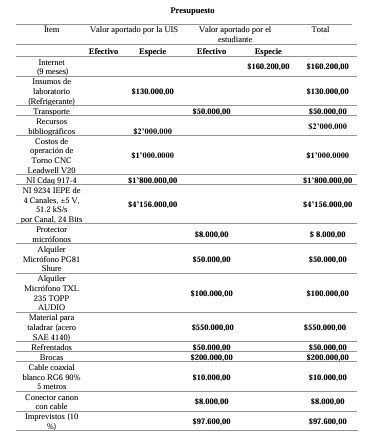
\includegraphics[width=\textwidth,keepaspectratio]{figures/presupuesto.png}\\[0.4em]

\includegraphics[width=\textwidth,keepaspectratio]{{figures/continuacion de presupuesto}.png}
\caption[Presupuesto del proyecto (tabla base del anteproyecto)]{Presupuesto base del proyecto: aportes UIS (efectivo y especie) vs. aportes del estudiante. Incluye operaci\'{o}n del Leadwell~V-20, cadena NI cDAQ-9174 + NI-9234, alquiler de micr\'{o}fonos PG81 y TXL~235, materiales (acero SAE~4140, refrigerante, brocas, cables) y horas de consulta/trabajo. Imprevistos al 10\,\%.}
\label{fig:presupuesto-uis}
\end{figure}

\begin{table}[htbp]
\centering
\small
\caption{Rubros adicionales del Lote~II no incluidos en el anteproyecto. Costos estimados en pesos colombianos (COP) a precios de 2026, asumidos en su totalidad por el estudiante (aporte en especie).}
\label{tab:presupuesto-art2}
\begin{tabularx}{\textwidth}{X c r}
\toprule
\'{I}tem & Unidad(es) & Valor (COP) \\
\midrule
Placa ESP32-WROOM-32 DevKit & 2 & \$\,70.000 \\
Micr\'{o}fono MEMS INMP441 & 2 & \$\,50.000 \\
Sensor de caudal YF-S201 & 1 & \$\,30.000 \\
Acoples hidr\'{a}ulicos y mangueras para el caudal\'{i}metro & 1 juego & \$\,40.000 \\
PCB prototipo 2~capas (fabricaci\'{o}n + env\'{i}o) & 5 & \$\,60.000 \\
Insumos de soldadura (esta\~{n}o, flux, pasta, puntas) & 1 kit & \$\,45.000 \\
Filamento PLA+ (rollo 1~kg) & 1 & \$\,95.000 \\
Filamento PET-G (rollo 1~kg) & 1 & \$\,110.000 \\
Impresi\'{o}n 3D del \textit{case} ESP32 y riel de micr\'{o}fonos & $\sim$60 h m\'{a}quina & \$\,80.000 \\
C\'{a}mara microsc\'{o}pica USB CMOS & 1 & \$\,90.000 \\
Cableado USB extensor y alimentaci\'{o}n & 1 juego & \$\,25.000 \\
Imprevistos Lote~II (10\,\%) & --- & \$\,69.500 \\
\midrule
\textbf{Subtotal Lote~II (aporte estudiante en especie)} & & \textbf{\$\,764.500} \\
\bottomrule
\end{tabularx}
\end{table}

Al sumar el subtotal del Lote~II al total del anteproyecto (\$\,13.673.800), el costo global consolidado del proyecto asciende a \textbf{\$\,14.438.300}~COP. La totalidad del incremento corresponde a aporte del estudiante en especie (electr\'{o}nica, consumibles, fabricaci\'{o}n aditiva y c\'{a}mara microsc\'{o}pica), sin impacto sobre los rubros desembolsados por la UIS.

%% ===== BIBLIOGRAPHY =====
\clearpage
\addcontentsline{toc}{chapter}{Referencias Bibliográficas}
\nocite{*}
\bibliography{informe_proyecto}

\end{document}